\documentclass[fr]{../../../eplsummary}

\usepackage{enumitem}
\usepackage[babel=true]{csquotes}

\hypertitle{Théorie des organisations}{5}{ECGE}{1317}
{Florian Thuin\and Héloïse Delvaux}
{Matthieu de Nanteuil}

\graphicspath{{res/}}

\section{Présentation du cours}

Trajectoire sociologique et historique des organisations. \newline


\textit{Qu'est ce qu'une organisation ?} Ce n'est pas nécessairement une
entreprise, une usine, un call center. C'est aussi une famille, une
université,\ldots C'est un segment quotidien de la vie sociale, dans
lequel nous agissons. L'organisation est un élément essentiel de notre
vie ordinaire : ce n'est pas seulement un lieu de production, qui est
piloté par une logique économique. Bien sûr, dans toute organisation, il
y a un problème économique de gestion, de rationalisation des ressources
en vue de réaliser un objectif, aussi large soit-il. Par exemple, une
université a pour objectif de rendre service à la société. Pour
accomplir ce but elle doit s'organiser. Si l'organisation ne réalise pas
ses objectifs, elle dysfonctionne. La dimension économique est une
dimension essentielle de l'organisation, quelle qu'elle soit. Dans tous
les cas, il y a une logique économique. \textit{Comment nommer cette
logique ?} \newline


Ce cours repose sur 3 éléments :

\begin{itemize}[label=$\bullet$]
    \item Une \textbf{conviction} : les organisations ne sont pas
        seulement des lieux de production de biens et services, mais ce
        sont aussi des lieux de construction de soi, des lieux de
        formation de notre « condition de sujet ». Ce sont des lieux où
        l'on se produit, par un travail sensé ou insensé.
    \item Un triple objectif :
        \begin{itemize}
            \item  Comprendre et montrer comment la notion d'organisation
            s'est progressivement construite. Cette notion n'est pas
            récente, mais elle a été profondément bouleversée après les
            Lumières.
            \item Montrer que les organisations sont des organisations
            humaines. On y fait l'expérience du travail. Elles façonnent
            les hommes et les femmes qui, par leur travail, participent
            à leur développement.
            \item Comprendre sans juger une part de la réalité qui est la
            nôtre, en nous aidant à critiquer le mode de développement
            libéral, capitaliste qui s'appuie sur des conceptions
            réductrices du travail, des organisations. Rendre compte des
            modes de rationalisation qui y sont à l’œuvre\ldots
    \end{itemize}
\item  Une \textbf{démarche compréhensive et critique}.
\end{itemize}
\bigskip

\textbf{Modalités d'évaluation} : matière = fiches et résumé des
articles de recherche

\begin{itemize}
    \item  Travail de groupe (50\%)
    \item  Stage d'initiation au monde du travail
    \item  Examen écrit (50\%) : 3 questions ouvertes (dont 2 longues),
        argumentation. Matière : synthèse des cas et fiches techniques
\end{itemize}
\bigskip

\textit{Livre à lire} : Si c'est un homme – Primo Lévi
Autres livres pouvant être consultés, mais non obligatoire

\section{Introduction}

Qu'est-ce qu'une organisation ? Qu'est-ce qu'un problème d'organisation
?

\subsection{Dédain pour la notion d'« organisation »}

Jusque dans les années 1950-60, la notion d'organisation n'avait aucun
intérêt, et renvoyait au monde du déterminisme, de la nécessité, voire
au monde animal.

\subsection{Quelques éléments d'étymologie}

\begin{itemize}
    \item Organon (gr.) ou organum (lat.) :organe du corps, voix,
        instrument (de musique) et ensuite, partie d'une machine
    \item Premières occurrences d'organe au 12 e siècle
    \item Organiser (14 e ) : disposer de manière à rendre apte à la vie
    \item Organisation (fin 14 e ) : vivant élémentaire animal et végétal
    \item Organique (14 e ), inorganique (15 e ), organicisme (19 e ) :
        Idée que tout comportement humain répond à des nécessités
        biologiques, vitales. Il y a donc un parallèle entre
        l'organisation sociale et l'organisation biologique. Dès le 19
        e, beaucoup de théories vont se développer sur le fait qu'une
        organisation est comme un corps humain, avec son métabolisme,
        ses fonctions, ses organes.
    \item Désorganisateur / Organisateur (1792) : terme plus politique,
        relatif à Robespierre. Quand ce terme entre dans la vie
        politique, c'est la désorganisation, le chaos qui fait peur.
        Suite à la révolution française. La désorganisation est une
        menace faite à l'ordre social. À l'inverse, « s'organiser » est
        un terme qui touche à la remise en ordre.
    \item Organigramme (1953)
\end{itemize}
\bigskip

On a donc d'abord une appréhension sur ce terme : c'est un dispositif
visant à organiser les fonctions vitales en se détachant du registre de
l'expérience immédiate et en répartissant l'autorité de la façon la plus
cohérente possible, en vue de maintenir l'ordre (social, politique,
culturel, etc.). Le terme « organisation » a souvent été comme une boite
noire, dans laquelle on ne pouvait pas rentrer, dont on ne sait pas très
bien ce que c'est. Mais aussi comme une boite blanche, un organigramme
(garant de l'ordre), desquels on connaît tout le fonctionnement. Au
final, ce n'est ni l'un ni l'autre ! Organisation = production, gestion,
et articulation entre les deux.

\subsection{Une variété de buts / finalités}

\begin{tabular}{p{0.48\linewidth}|p{0.48\linewidth}}
    \centering Organisation animale & Organisation humaine \\
    \hline
    Connotation organique, biologique, orientée vers la survie, vers la
    reproduction de la vie, de façon parfois complexe (ex : meutes,
    ruches). Réelle organisation, avec comme but de reproduire la vie.
    Les animaux n'ont pas la capacité de définir par eux mêmes les buts
    qu'ils vont poursuivre : leurs buts sont déterminés. &
    Complexité toute autre, qui n'est pas seulement technique ou
    fonctionnelle en vue de reproduire la vie, mais dont on sent qu'elle
    va recouvrir des dimensions multiples (économiques, politiques,
    culturels,\ldots). Les buts d'une organisation humaine ne sont par
    déterminés mais auto déterminés, par ceux qui sont au cœur de
    l'organisation. Ce sont les buts que l'on se donne dans un contexte
    qui caractérisent l'organisation humaine. \\
\end{tabular}

Le premier grand type d'organisation humaine est essentiellement à
finalité politique (+ à finalité sociale), comme par exemple dans le cas
de la cité grecque (voire plus ancienne au 4e, 5e siècle avant JC). Les
buts de la cité sont de se protéger contre les adversaires et de se
protéger soi même à partir d'un principe d'égalité. La question de la
guerre (organisation) est fondamentale dans la genèse de l'organisation.
\newline


Il y a ensuite un changement radical : Avec la naissance de l'économie
de marché, les finalités économiques deviennent les principales
finalités poursuivies. Avant ça, on survivait pour vaincre, pour exister
en tant que cité. Le moment de basculement dans la monde est quand la
finalité économique devient la finalité exclusive et principale des
organisations. Ce changement dans l'ordre des finalités est récent.
Attention ! Cette finalité économique n'est pas spécialement une
finalité marchande, sanctionnée, régie, évaluée par un marché
(l'économie de marchés n'est pas la seule économie viable !). En effet,
le marché dépend de nombreuses institutions, et il existe un tas
d'organisations qui se situent à la périphérie du marché, ou qui ne se
situent pas sur un marché. La finalité économique est souvent marchande,
mais elle peut être non marchande. \newline


Les organisations sont dans un \textbf{cadre institutionnel} : elles se
déterminent dans un contexte. Quelle que soit sa taille ou sa finalité,
une organisation agit en contexte, sous contraintes par des institutions
d'enseignement, politiques, de santé, etc. Càd par des grands mécanismes
qui déterminent les règles de la vie collective dans une société. Ce
n'est pas l'organisation qui décide de tout. Quelle qu'elle soit,
l'organisation agit dans un contexte institutionnel.

\subsection{Trois notions de bases}

Trois dimensions vont rythmer le cours. Ce sont des notions
constitutives de la théorie des organisations.

\begin{description}
    \item[Rationalité] : S'organiser, c'est d'abord sortir du chaos,
        mettre de l'ordre, planifier, prévoir, anticiper, bref, c'est
        faire preuve de rationalité.
    \item[Travail] : Ce principe ne s'applique ni à l'amour, ni à la
        guerre,\ldots mais aux activités de production de biens et de
        services au sein d'une collectivité. Il désigne aussi bien les
        caractéristiques générales du travail (durée, condition,
        organisation) que l'activité de travail elle-même.
    \item[Subjectivité] : Une organisation n'est rien si on la sépare
        des personnes concrètes qui y participent. Une organisation ne
        gère pas seulement des ressources techniques, mais elle gère
        aussi des relations, des liens entre ces actions. Ce sont ces
        personnes qui, par leurs décisions ou leurs engagements
        réciproques, façonnent l’organisation au quotidien. Vivre
        subjectivement les choses, c'est en faire l'expérience.
\end{description}

Dans la tradition sociologique, on désigne ces personnes comme des «
sujets », individuels ou collectifs. Lorsque les « sujets » sont
examinés du strict point de vue de leur implication dans une action
collective, on privilégie le terme d’ « acteur ». En effet, pendant
longtemps, on a considéré que les hommes et les femmes qui s'activent
pour produire peuvent être appelés des acteurs sociaux. Le terme
d'acteur est un peu court. Car cette notion sous-estime le fait que,
dans une organisation, il y a une manière de travailler, de vivre le
travail en relation à d'autres qui sont extrêmement variantes. On n'y
agit pas simplement pour l'organisation. Mais on fait aussi une
expérience de travail, qui est une expérience de vie. En faisant cette
expérience, on est en étroite relation avec d'autres. On y fait
l'expérience du sens et on se pose une question sur la signification.
\newline

On parle donc de sujets plutôt que d'acteurs car :
\begin{itemize}
    \item Nous faisons l'expérience du travail ; nous vivons comme les
        sujets d'une expérience vécue corporellement, émotionnellement. 
    \item Dans les relations que nous avons avec autrui, nous sommes
        dans des relations de reconnaissance, d'estime ou de mésestime
        réciproque. Nous nous jugeons les uns les autres.
    \item Une question du sens se pose : pour nous en tant que sujet,
        nous éprouvons le réel, nous attendons d'autrui une certaine
        reconnaissance, mais nous nous posons aussi la question du sens
        de ce que nous faisons.
\end{itemize}

Il s'agit donc d'un triangle au cœur de l'analyse des organisations.
L'organisation est la mise en place de ces 3 principes :

\begin{itemize}
    \item Rationalité
    \item Travail : cette volonté de mettre en œuvre dans la vie sociale
        des critères de rationalité s'applique essentiellement au
        travail. 
    \item Subjectivité : cette manière d'organiser le travail ne peut
        pas se faire sans la présence de personnes concrètes, sans la
        présence de sujets.
\end{itemize}

Est-ce que c'est suffisant ? Non ! On doit reconnaître que le terme de
rationalité doit être en quelques sortes dédoublé. Il existe non pas une
mais deux rationalités. D'un coté ce qu'on appelle la rationalité
formelle et de l'autre une rationalité substantielle. Une organisation
est une mise en relation entre travail, subjectivité, et deux types de
rationalité. Sur quoi repose cette distinction en les 2 rationalités ?
Pourquoi cette distinction est-elle importante ?

\begin{itemize}[label=$\diamond$]
    \item La \textbf{rationalité formelle} est typiquement celle à laquelle nous
        sommes formés. Elle met l'accent sur la conformité des choix à
        une procédure de calcul ou de droit, ainsi que sur la cohérence
        formelle de cette procédure. On parle de rationalité lorsque
        l'on est capable de faire état d'une procédure de calcul, ou
        quand on est capable de se référer à une règle de droit. Ces
        éléments présentent une forte dose de rationalité. Ils reflètent
        cette idée de raison ou de rationalité ; mais ils n'en reflètent
        qu'une part, soit notre capacité à nous conformer à des règles
        de calcul ou de droits, qui ont été définies préalablement à
        toute situation concrète. En ce sens, il s'agit d'une
        rationalité formelle, car il s'agit de se conformer à la forme
        du raisonnement économique (calcul) ou juridique (droit) plutôt
        qu'à la singularité, qu'à la particularité d'une situation
        concrète. Dans le cas d'une procédure de calcul, la rationalité
        formelle s'appuie sur l'utilisation de méthodes de
        quantification de la réalité, dans le cadre d'une démarche
        \textbf{coût/bénéfice, force/faiblesse, avantages/inconvénients}. Cette
        méthode est relativement récente. Elle date de la naissance de
        l'utilitarisme. La rationalité économique qui repose sur la
        généralisation des procédures de calcul considère que toute
        expérience que nous faisons du monde peut faire l'objet d'une
        quantification entre des bénéfices et des coûts. On parle aussi
        de rationalité calculatrice. L'organisation marchande
        (entreprise privée) est lieu qui, parce qu'elle est réglée par
        un marché, est un cas dans lequel cette rationalité est
        généralisée. \newline

        
        Parallèlement, on peut aussi distinguer une rationalité
        juridique, qui consiste à se référer à un corpus de règles,
        définies à priori. Ces règles ont un caractère durable et
        contraignant. À la différence de l'organisation marchande, c'est
        l'organisation publique ou bureaucratique (une administration)
        qui est le lieu dans lequel cette rationalité va se généraliser.
        \newline


        Il existe des types d'organisation qui sont idéaux, dans
        lesquels ce type de rationalité (de calcul ou de droit) est la
        norme. Il y a tout un pan de la vie sociale, dans la modernité
        industrielle de façon indispensable, qui relève de la
        rationalité formelle.
\end{itemize}

Est ce que ce type de rationalité va suffire pour définir l'idée de
rationalité ? Non ! La rationalité formelle n'est pas la seule acception
possible de la rationalité. \newline


Exemple : quand on travaille en groupe, quand on doit coopérer avec les
autres, faire confiance à des personnes (appelées plus tard des
collègues) qu'on ne connaît pas, et qu'on ne connaîtra pas sur le plan
personnel, est-ce irrationnel, déraisonnable ? On voit bien que
lorsqu'on coopère avec quelqu'un, on ne se conforme à aucune règle de
calcul ou règle de droit. Le fait d'entrer en relation avec d'autres
entraîne forcément un comportement irrationnel ? \textbf{Non}. On
développe un savoir faire, une logique qui ne relève pas de la
rationalité formelle (on ne se conforme ni au calcul ni au droit) mais
on n'agit pas de façon incohérente ou irrationnelle\ldots Entrer en
relation avec d'autres, dans la vie sociale comme au travail, se fait de
façon rationnelle. \newline


Quand on entre en relation avec d'autres, on développe :

\begin{itemize}
    \item une capacité à rester cohérent
    \item une capacité à faire appel à une argumentation, qui sous-tend
        notre relation aux autres
    \item on demeure soumis à la volonté humaine – individuelle ou
        collective -, même si celle-ci est évolutive, complexe et
        parfois obscure.
\end{itemize}
\bigskip

Il y a donc un autre type de rationalité qui sous tend l'idée de
rationalité formelle :

\begin{itemize}[label=$\diamond$]
    \item La \textbf{rationalité substantielle} est l'idée qu'il faut
        privilégier la relation, l'interaction en tant que telles et le
        sens que cette relation a pour nous. La rationalité
        substantielle porte sur les relations et sur leur sens. Cette
        rationalité ne renvoie pas à un type d'organisation, mais elle
        est présente dans toutes. Elle n’est pas « moins rationnelle »
        que la rationalité fondée sur le calcul ou le droit : elle est à
        la fois différente et complémentaire. Elle est présente dans
        toutes les organisations.
\end{itemize}
\bigskip

Dans la cité grecque ou l'abbaye médiévale, la norme n'est pas la
rationalité formelle, càd se conformer à des règles de forme de calcul
ou de droit. Ce qui importe, c'est le sens des relations humaines, en
référence à un Créateur. Que se passe-t-il avecle passage à la modernité
? Ce n'est pas seulement l'avènement de la démocratie, de l'économie de
marchés, etc. C'est plus profondément un \textbf{renversement
anthropologique fondamental} dans l'idée que l'Homme se fait de
lui-même. Un renversement selon lequel ce qui importe est la capacité à
se conformer à des règles de calcul ou des règles de droit, et plus le
contenu ou le sens des relations humaines. C'est un changement radical.
\newline


Au-delà des différences terminologiques, il existe une différence
épistémologique entre ces deux types de rationalité, ainsi que l'a
montré Max Weber (Économie et société) :

\begin{itemize}
    \item La première est dite « univoque », car elle ne donne lieu qu'à
        un seul type d'interprétation possible (fixée par la procédure
        de calcul ou de droit) : elle marche ou elle ne marche pas. On
        se conforme ou on ne se conforme pas.
    \item La seconde est dite « équivoque » (ou « plurivoque ») car elle
        ouvre sur une infinité d'interprétations possibles. Elle porte
        sur les dimensions de l'action humaine dont il n'est pas
        possible de fixer le contenu une fois pour toutes\ldots bien
        qu'elles soient guidées par un certain usage de la raison. Il y
        a plusieurs manières de rendre compte de la question de
        confiance. La rationalité substantielle est infiniment ouverte ;
        elle ne relève pas d'une conformité à une procédure définie
        antérieurement.
\end{itemize}
\bigskip

Ainsi : le travail en équipe, la capacité à diriger, le sens du travail
bien fait, l'engagement collectif, le conflit, la confiance,
l’autoritarisme, la capacité à déléguer, la reconnaissance, la
disqualification, la gestion de projet, la rétention d'informations, la
solidarité, le repli sur soi, la confrontation interculturel, le désir
ou le refus de changer, la passion\ldots relèvent de ce type de
rationalité. \newline


La \textbf{coopération} repose sur des liens de confiance, nécessaires
au succès économique d’une organisation : peut-elle se calculer,
est-elle irrationnelle ? \newline

En réalité, il est très important de comprendre que ces différents
aspects, s’ils reposent sur des relations, ne relèvent pas pour autant
de l’irrationnel ou de la déraison :

\begin{itemize}[label=$\bullet$]
    \item ils sont relativement cohérents ;
    \item ils font appel à une argumentation spécifique, même si
        celle-ci ne passe pas par la formalisation mathématique ou
        juridique ;
    \item ils demeurent soumis à la volonté humaine – individuelle ou
        collective –, même si celle si est évolutive, complexe et
        parfois obscure !
\end{itemize}
\bigskip

\fbox{\begin{minipage}{\linewidth}
    \textit{Remarque :} Un paradigme est une vision partagée du monde
    qui regroupe un ensemble de théories. Il arrive de changer de
    paradigme, quand on découvre d'autres théories. Il y a une pluralité
    des paradigmes, qui vont se développer au cours du temps. Il existe
    plusieurs grilles de lecture du monde.
\end{minipage}}
\bigskip

Pourquoi la distinction entre \underline{rationalité formelle} et
\underline{rationalité substantielle} est elle importante ? Parce
qu'elle désigne \textbf{deux rapports distincts à la performance}.
\newline

« Performance » : origine étymologique anglaise.

> to perform : terme utilisé au théâtre) qui signifie « réaliser une
performance », « rendre visible », « exhiber », « mettre en scène », «
accomplir »,\ldots Ça a trait à un mode d'apparition en public. C'est
par extension que ce terme est devenu synonyme d'efficacité. Il y a un
contexte de compétition dans lequel l'efficacité est évaluée, et dans
lequel celui qui est performant est jugé plus efficace. \newline

$\rightarrow$ On passe d'un terme théâtral à un terme économique. Il y a
donc non pas un mais deux sens possibles à l’idée d’une organisation «
performante » :

\begin{itemize}
    \item On peut dire qu'une organisation est performante quand elle
        atteint un haut degré d'efficacité, autrement dit lorsque la
        conformité aux règles de calcul ou de droit lui permet d'assurer
        les finalités qui sont les siennes plus efficacement que ses
        concurrents (rationalité formelle).

        Ex : Une bureaucratie, une administration doit être efficace :
        elle doit avoir la capacité à maintenir l'ordre des règles
        qu'elle a pour objet de surveiller ou de faire appliquer. Une
        bureaucratie est efficace dans la mesure ou elle permet à un
        nombre de règles de se perpétuer.
    \item Une organisation performante, au sens « théâtral » du terme,
        est une organisation qui rend visible les interactions sociales
        sur lesquelles elle repose, et le sens que les sujets donnent à
        ces interactions. Or, sur ce plan, une organisation est toujours
        performante : sa performance ne dépend pas d’une position de
        concurrence, mais d’une manière de mettre à jour, de « modéliser
        » le tissu social sur lequel elle fonde son développement
        (rationalité substantielle). L'organisation est toujours un lieu
        qui fait voir un certain type de rapports sociaux. Elle n'est
        donc pas seulement performante au plan économique (ce qui
        sous-tend la rationalité formelle) : elle peut être performante
        au plan social, quand elle rend visible des rapports sociaux,
        des significations sociales.
\end{itemize}

La première définition de la performance (s'appuyant sur une rationalité
formelle) suppose qu'il existe des dispositifs d'évaluation de la
performance (ex : marché, ordre politique ou juridique). Sur le plan de
la performance sociale, il n'existe pas de dispositif d'évaluation
externe à la performance. Une organisation est toujours performante sur
le plan social dans la mesure ou elle fait apparaître des situations
sociales. Elle permet de modéliser le tissu social. C'est parce qu'il y
a de la substance dans les relations engagées les uns envers les autres
(sous contrainte d'efficacité) qu'on doit se pencher sur ce qui est
produit, dans ces relations. \newline


Une recherche de référence « Les mondes sociaux de l’entreprise » [par
R. Sainsaulieu, Isabelle Francfort, Florence Osty et Marc Uhalde (1995),
puis Florence Osty et Marc Uhalde (2007)]. L'ouvrage dit qu'il n'y a
\textbf{pas de schéma idéal} (ce qui est contre ce que dit la théorie
des organisations). Il y a en réalité 5 types d'organisations /
d'entreprises :

\begin{itemize}[label=$\bullet$]
    \item L'entreprise bureaucratique / la bureaucratie négociée ou modernisée. 
    \item L'entreprise communauté, soit l'entreprise familiale dans
        laquelle tout le monde partage la vie de travail ou hors
        travail, dans laquelle la dimension affective est très forte,
        dans laquelle il y a une histoire, etc.
    \item L'entreprise en crise : qui connaît une cassure dans son
        développement.
    \item L'entreprise modernisée, qui a réussi à mettre en place un
        haut niveau de technologie.
    \item L'entreprise duale, càd coupée en deux, qui est d'un côté très
        performante sur le plan économique, mais au sein de laquelle les
        relations sociales, l'atmosphère sont déplorables. C'est une
        entreprise dans laquelle les conditions sociales sont minimales,
        suivant un peu le modèle de l'entreprise taylorienne.
\end{itemize}
\bigskip

Cette recherche montre qu'il n'y a pas d'entreprise idéale, ni
d'articulation définitive entre ce que l'on vit au travail, et la
performance économique du travail. \newline


Le rôle de ce cours est d'interpréter les mondes sociaux qui traversent
n'importe quelle organisation. Il existe une pluralité d'interprétations
de ces mondes sociaux. Il ne faut pas oublier le coût, la substance
social(e) de la performance économique. \newline


\begin{figure}[!ht]
    \centering
    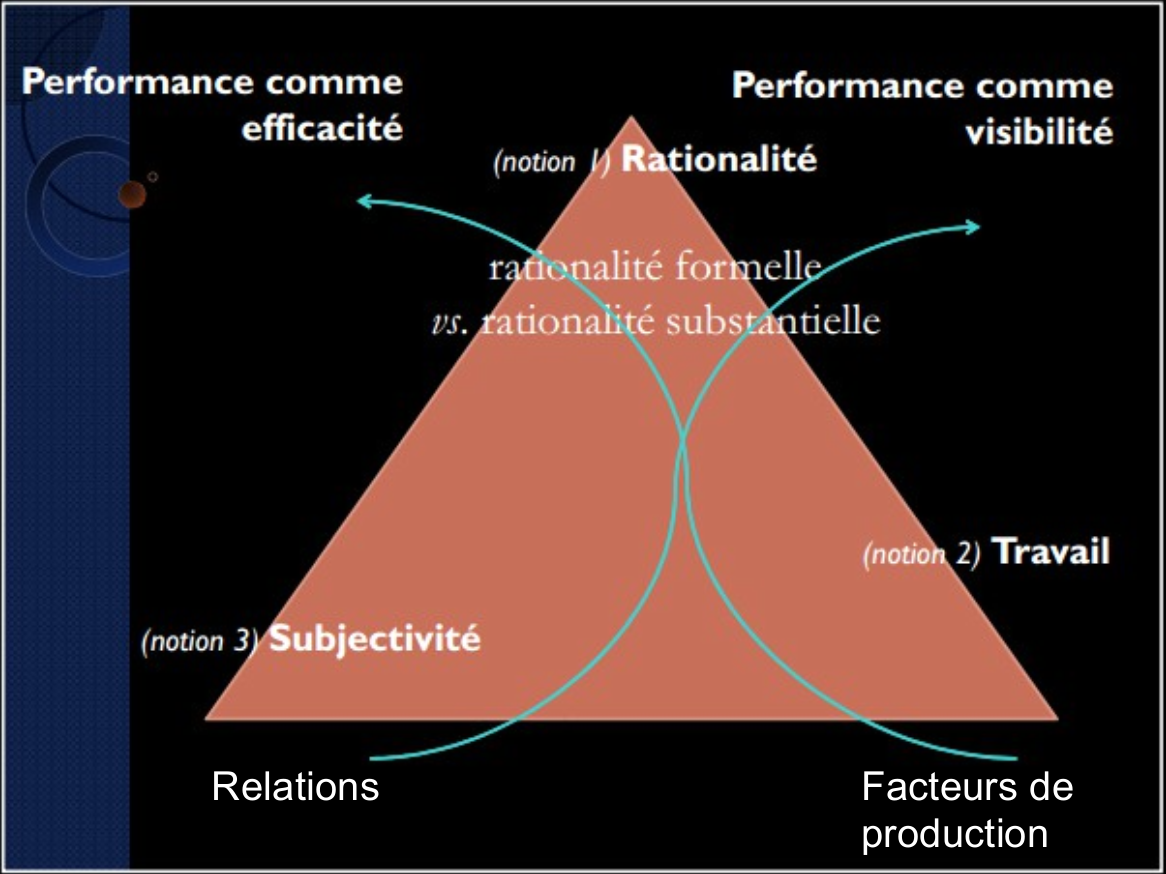
\includegraphics[width=0.75\linewidth]{triangle_fleches.png}
\end{figure}

Si la théorie des organisations s'appuie sur un triptyque
(rationalité-travail-subjectivité), elle met en lumière deux rapports à
la performance :

\begin{itemize}[label=$\bullet$]
    \item La performance comme efficacité : on part du travail comme
        facteur de production, sans relations de travail (situé à
        l'extrême sur la courbe « facteurs de production » quand elle
        est toute seule (dans certaines entreprises)).
    \item La performance comme visibilité de la réalité sociale (courbe
        « relations »)
\end{itemize}
\bigskip

Une grande partie de la pensée sur les organisations (la tradition
utilitariste, l’école des relations humaines (années 1950-1960), divers
courants de la gestion des ressources humaines (années 1980-2000), sans
oublier les essayistes en tout genre qui font fleurir les rayonnages de
management) fait l’hypothèse que ces deux acceptions de la performance
sont \underline{complémentaires} : sinon à court terme, du moins à plus
long terme. \newline


En effet, être bien à son boulot entraîne une grande performance
économique. La performance économique d'une organisation suppose donc
qu'elle repose sur de bonnes relations de travail entre les
travailleurs. Cette hypothèse a été défendue par différentes écoles.
\textbf{Dans la réalité, cette hypothèse n'a pas pu être vérifiée}.
\newline


Dans les faits, rien n’est moins sûr :

\begin{itemize}[label=$\bullet$]
    \item Non seulement parce que des recherches comme celles que nous
        venons citer le prouvent,\ldots
    \item \ldots mais surtout parce qu’il n’existe pas de théorie
        permettant de proposer un mode d’articulation général et
        définitif de ces deux types de performance.
\end{itemize}
\bigskip

L’important est ailleurs : il est de chercher à comprendre quels types
de relations sociales s’articulent à quel type d’efficacité et ainsi
d’ouvrir la discussion sur ces deux types de réalité. Il n'y a donc pas
de relation de cause à effet entre ce que les gens vivent au travail, et
la performance économique. Le retour de l'organisation taylorienne en
Europe, aux USA, en Chine, dans les pays du Sud montrent au contraire
que certaines organisations très performantes économiquement le sont au
détriment du salariat\ldots Il n'y a pas de lien de cause à effet entre
ces types de performance, car ils renvoient à deux types distincts de
rationalité, deux niveaux distincts de la réalité. Rationalité formelle
et rationalité substantielle sont deux réalités différentes ! \newline


Il s'agit donc de deux niveaux, deux plans distincts : l'une n'est pas
supérieure à l'autre. Le problème d'un certain type d'économie (économie
politique ou économie néoclassique) est qu'il considère que la seule
rationalité valable est la rationalité formelle, et qu'elle est donc
meilleure que celle qui a trait aux relations sociales. C'est une erreur
logique, factuelle, normative (au sens de ce qui doit être). À
l'inverse, la rationalité substantielle n'est pas meilleure : elle
décrit le monde différemment. \newline


Dans le paradigme utilitariste, le travail est un facteur le production,
voire le facteur de production. Dans cette vision-là, on ne considère
jamais vraiment les travailleurs comme des personnes, et on ne considère
jamais vraiment sérieusement les relations entre eux. Le travail n'est
donc pas seulement un facteur de production, mais un lieu dans lequel
des sujets peuvent s'accomplir. De plus, Max Weber dit que les
travailleurs doivent voir le travail comme vocation. Il considère que
cela est permis par la naissance du protestantisme (avec la rupture
vis-à-vis du catholicisme). Ce point de vue ouvre sur une contradiction,
car le capitalisme dans son développement et dans la façon dont il va
organiser le travail, va en quelques sortes se retourner contre les
travailleurs. \newline


De façon synthétique, on retiendra cette définition de l’organisation :
\newline


\textit{\enquote{Une organisation est une configuration de personnes et
de ressources créée pour coordonner une série d’activités
professionnelles, dans le but d’atteindre des objectifs ou de produire
des résultats » (Fischer \& Lovell, 2006). Mais on lui adjoindra la
précision suivante : « c'est un ensemble de conduites ‘‘rationnelles’’
engagées dans des rapports mutuels, pour lequel il n’existe pas de
théorie générale permettant de prédire le sens de cette combinaison}}.

\subsection{La démarche du cours : une perspective historique, une
pluralité de grilles de lecture (« paradigmes »)}

Figures de l'organisation pré-moderne :

\begin{itemize}
    \item La cité grecque
    \item L'abbaye médiévale
\end{itemize}
\bigskip

Ces dernières ne sont pas des organisations capitalistes. Le capitalisme
est né à la fin du 18e siècle, bien qu'il ait des précédents au 16ème
siècle (avec le mercantilisme). Il y avait également des organisations
proto-capitalistes en Asie. Cependant, le capitalisme que nous
connaissons aujourd'hui prend son essor en Europe (plus précisément en
Angleterre) au 18ème siècle, sous des modalités très précises. \newline


Les organisations étudiées ici, sont des organisations
\textbf{pré-capitalistes} et \textbf{pré-modernes.} \newline


Si on considère que l'économie politique classique va asseoir la
supériorité de la rationalité formelle sur la rationalité substantielle,
alors il faut comprendre les organisations pré-modernes, comme des
organisations qui soit ignoraient la rationalité formelle, soit la
plaçait sous la coupe de la rationalité substantielle. Dans les
organisations pré-modernes, les relations sociales et le sens de ces
relations ont plus de sens que la rationalité formelle, juridique ou
économique. Par exemple, dans l'Antiquité romaine, il y a la
\underline{maison du maître} (qui renvoie à toute une organisation de la
sphère privée - entre le maître, sa femme, ses esclaves) et
l'\underline{armée} (organisation qui apparaît comme quasi idéale). Dans
ces types d'organisation, ce qui prime n'est pas la rationalité
économique ou la norme juridique. Ce qui prime est un système de
relations sociales. \newline


Dans la Grèce antique, Même si une cité est vouée à mourir de faim ou à
vivre dans de mauvaises conditions, l'importance pour les grecs est la
\textbf{concertation}. Dans les grands ordres médiévaux, ce qui importe est la
consécration, le sacrifice de soi en faveur de l'ordre (qui renvoie à
une vision religieuse, métaphysique du monde). C'est aussi le fait que,
dans ces abbayes, on voit apparaître un ordre social particulier mais
dont la finalité est toujours une finalité religieuse ; et c'est la
raison pour laquelle, on y travaille (faire de la bière) afin d'occuper
les moines pour la consécration de soi à Dieu (et pas pour gagner de
l'argent). Dans ce cadre, la rationalité formelle est toujours
\underline{seconde}. \newline


Du même coup, on comprend que la naissance de l'économie moderne n'est
pas seulement un changement dans l'organisation du monde, du point de
vue de la production et la distribution matérielle. C'est plus
profondément un changement au plan de la vision, de la représentation
que nous nous faisons d'un monde humain rationnel. D'un coup, l'idée de
raison va se trouver \textit{\underline{bouleversée}}. C'est un
changement dans le type de rationalité qui est mobilisé, un changement
dans la vision de l'homme, un changement des paramètres les plus
fondamentaux. \newline


\subsubsection{La cité grecque}

Au plan philosophique, la cité grecque a posé tous les jalons de la
philosophie (Platon, Aristote,\ldots). Comment s'organisaient les Grecs
? \newline


La cité (type d'organisation essentiel de l'époque) est un espace clos,
autarcique qui prétend vivre de lui-même, de ses ressources, de son
activité et qui se conçoit comme une fin en soi, sans rapport direct
avec l’extérieur : un « pays » est d’abord une collection de cités
organisées et prospères, rivales et, le plus souvent, en guerre. La cité
désigne un premier moment d’organisation de l’espace et du temps : la
Cité fait apparaître une organisation complexe des personnes, des lieux,
des objets\ldots \newline


Quels en sont les principales caractéristiques ? \newline


Athènes est le point de départ de toute la pensée démocratique. «
\textbf{Un Athénien est un homme libre} » : la Cité est l’assemblée des
citoyens libres. Son organisation repose à la fois sur une
\underline{règle d’appartenance} (accès à l’assemblée ou « ecclesia »,
droit de vote, devoir de participation) et sur une \underline{règle
d’exclusion} (artisans, commerçants, femmes, esclaves). \newline


Il y a dans l'Antiquité grecque l'idée fondamentale que la cité, soit
l'espace public du politique, est d'abord le lieu ou se réunissent des
citoyens libres. Des citoyens sont des personnes dotées d'une identité
politique, et qui en tirent des droits. ''Libre'' veut dire qu'ils
peuvent se consacrer à la discussion sur l'avenir qui leur est commun.
Entre ces citoyens libres, il y a un principe d'égalité stricte. Chacun
est reconnu comme étant l'égal de l'autre, ayant les mêmes droits. Ces
hommes sont propriétaires d'un domaine, à la tête d'une hiérarchie faite
de femmes et d'esclaves. Être un citoyen libre, c'est être libre – ou
plutôt libéré – des préoccupations de gestion des choses matérielles,
des préoccupations économiques. L’assemblée des citoyens libres regroupe
ceux qui ont la possibilité de s’élever au-dessus des contingences
matérielles, au-dessus du règne de la « nécessité ». Il y a donc un
mépris pour les activités « nécessaires », vouées à la production et à
la reproduction, un principe de rejet. Trois exclusions : \newline

\begin{itemize}
    \item Les femmes : elles assurent le « travail reproductif » et sont
        liées par les activités de soin (des enfants) et d’entretien
        domestique (de la maison). Elles peuvent toutefois exercer une
        influence sur le maître de maison, et en tirer un certain
        pouvoir.
    \item Les esclaves : ils ont en charge la production des basses
        besognes. Ils sont liés par la matière. Leur statut social est
        conforme au rôle qu'ils occupent dans la cité.
    \item Les artisans, les commerçants et les paysans : ils sont
        concrètement dans la cité. Ils sont moins rejetés que les
        esclaves, mais ils ne sont pas autorisés à entrer dans l'agora.
        Concernant les paysans, l’activité agricole naît d’un «
        éloignement progressif des dieux ». L’artisan, lui, exerce une
        activité « qui peut aller jusqu’à impliquer les trois
        dépendances de la nature, des usagers et du maître ». Le
        commerçant fait, quant à lui, l’objet d’une suspicion
        généralisée car il incarne, plus que les autres, « l’envie
        illimitée » de la richesse.
\end{itemize}

Le travail est hors les murs. Dans la Grèce ancienne, on est soit
citoyen, soit travailleur. \newline


Ainsi, la situation économique et sociale n’a pas d’incidence directe
sur la participation à la vie publique : bien sûr, il y a des riches et
des pauvres et, entre ceux qui sont admis au rang de citoyen, des
différences de richesses. Mais la richesse n’est pas un objectif en soi.
\newline

Elle répond à trois fonctions spécifiques :
\begin{itemize}
    \item Elle permet d’abord d’acquérir des honneurs
    \item Elle crée également des obligations – elle ne peut pas
        permettre de s’affranchir des sanctions qui régissent l’accès
        aux charge publiques.
    \item Enfin, elle donne accès au statut que confère le fait d’être
        libéré des contraintes du travail.
\end{itemize}

\textbf{Qui sont alors ceux qui ont « droit de cité » ?} \newline


Ce sont les maîtres de maison, des personnes de sexe masculin qui vivent
de leurs rentes et sont propriétaires d’une maison (domus) sur laquelle
ils exercent leur autorité. À l’inverse, les artisans, les commerçants,
les femmes et les esclaves n’ont pas accès aux charges publiques : ce
sont des « citoyens de seconde zone ». La Cité est enfin le lieu du
discours, de la rhétorique, du théâtre. Ce qui véritablement structure
les rapports entre les citoyens est leur faculté de « jouer un rôle »
sur la scène publique, de convaincre (« harangues »), d’être aimé ou
haï\ldots L’organisation repose donc sur la théâtralisation du corps des
personnages publics, libérés des entraves de la vie matérielle par le
support des « autres » qui, eux, se voient privés du titre de citoyen.
\newline

Comment la rationalité formelle s'applique-t-elle à la cité grecque ?

\begin{itemize}[label=$\bullet$]
    \item La \textbf{rationalité formelle} est quasiment inexistante, dans le
        sens ou la cité est guidée par une finalité spécifique («
        rationalité substantielle »), celle de la pratique démocratique
        du pouvoir en vue du bonheur. L’administration ou le commerce («
        rationalité formelle ») y jouent un rôle marginal, du moins en
        tant que principes organisateurs de la vie collective. Si la
        rationalité formelle est inexistante, la rationalité
        substantielle est toute puissante : c'est elle qui fixe les
        règles de la cité.
    \item Le \textbf{travail} est une activité qui relie l'humanité au monde
        animal. Le travail est explicitement situé hors-les-murs de la
        Cité : travailler s'oppose au fait de devenir citoyen et être
        libre revient donc à ne pas travailler, à pouvoir être dispensé
        du travail sur la matière, à se définir comme « animal politique
        » (Aristote). La cité est une organisation sans travail, une
        cité dont les principes excluent ce dernier. Si on travaille, on
        n'aura pas accès au cœur de la cité : l'agora. La Cité est donc
        la mise en scène de rapports entre les personnes, dont le sommet
        est constitué par ceux qui ont la charge de définir ses grandes
        orientations et de pourvoir au « bonheur » du plus grand nombre.
    \item Qui en sont les citoyens ? Ce sont des hommes maîtres de
        maison. Ils s'identifient pleinement aux finalités de la cité.
        Si l'on appliquait le terme de sujet, on parle d'une forme de
        subjectivité, càd une manière de faire l'expérience de la cité.
        Mais cette expérience est clivée selon le rang et selon le sexe
        : seules les propriétaires, de sexe masculin ont accès à la Cité
        et en tirent une définition positive d’eux-mêmes. Ces citoyens
        existent donc subjectivement à travers leur appartenance à un
        ensemble plus vaste qu’eux-mêmes, à un « monde objectif » (la
        Cité, mais aussi le territoire et le cosmos). En toute rigueur,
        on doit dire que leur identité est intrinsèquement liée aux
        finalités de l’organisation. Cela ne signifie nullement qu’elle
        soit inexistante : par le théâtre et l’usage public de la
        parole, elle fait au contraire voir des personnages, dont les
        vêtements et la parure sont un élément-clé de leur « apparition
        sur scène » (en particulier dans « l’ecclesia »). Le corps est
        ici le support explicite à partir duquel l’organisation prend
        forme et s’actualise. Il importe toutefois de  préciser ceci :
        dans l’assemblée des citoyens libres, les hommes-propriétaires
        sont admis en raison de leur statut. Les autres en sont exclus.
        Il en découle un point important : l’appartenance à la Cité –
        réservée aux hommes-propriétaires – se fait sans médiation
        hiérarchique. On en est\ldots ou on en est pas. C’est là, sans
        doute, que réside l’intuition démocratique la plus fondamentale
        que les Grecs aient inventé : la Cité est une assemblée d’égaux.
        La hiérarchie sociale concerne ceux qui, par le lien avec le
        règne de la nécessité, en sont exclus. Même si elle concerne le
        plus grand nombre, la hiérarchie se situe à la périphérie de la
        Cité. Cela ne signifie nullement que la société soit homogène.
        Comme l’écrit Alain Cotta (texte du syllabus) : « Cette relation
        des citoyens et des esclaves condense la structure sociale de la
        Cité grecque, mais ne la résume pas. La société n’est pas duale.
        Entre le sommet et la base, la hiérarchie sociale détend sa
        complexité : esclaves affranchis, salariés, hommes libres,
        métèques, thètes, artisans, commerçants. Chacune de ces strates
        présente elle-même ses multiples dissociations, aux incessantes
        évolutions, selon les guerres publiques et civiles, les troubles
        politiques, les vicissitudes économiques. Mais il n’en demeure
        pas moins que l’ordre social est bâti à l’encontre du travail .
        (\ldots) La Cité naît de  l’exclusion du travail hors-les-murs
        ».
\end{itemize}
\bigskip

\subsubsection{L'abbaye médiévale}

L'abbaye de Cluny au XI e et XII e siècle est une organisation
religieuse prestigieuse au cours de la période du Haut Moyen-Âge. Il
s'agit là d'un exemple typique, d'un « idéal-type ».

\begin{itemize}
    \item des « \textbf{buts de mission} » : la finalité de l’organisation, sa raison d’être ;
    \item des « \textbf{buts de système} » : la gestion des moyens de production,
        le contrôle des ressources, le maintien de l’ordre, etc.
\end{itemize}
\bigskip

Hypothèse générale de l’auteur : les « buts de système » jouent un rôle
grandissant dans la finalité de l’organisation et dans sa pérennité.
\textit{Comment} ? \newline


Il y a un problème de l’autorité de la maison-mère sur « des centaines
de maisons », càd une préoccupation croissante pour les ressources, des
scissions, des conflits, mais aussi une évolution doctrinale. Les
activités agricoles (possession de différents domaines nécessaires à
l’entretien des moines) sont un effort économique soutenu (rôle de «
l’argent ») et apparaissent comme des relations avec l’extérieur sous la
forme de « dons contre prières ». Les personnes vivant dans l'abbaye
sont réparties en trois catégories : \newline

\begin{enumerate}
    \item les moines (issus de la moyenne ou petite noblesse)
    \item les « frères lais » ou « convers »
    \item les serviteurs.
\end{enumerate}
\bigskip

Cette hiérarchie sociale se trouve dans l’organisation elle-même, en
fonction à la fois du rang d’origine et de la fonction dans l’abbaye.
\newline


Choix de l’Abbé (maison-mère) et des prieurs (autres maisons) : élection
ou désignation ? Les pratiques évoluent et se différencient. Cette
évolution n’est pas de nature doctrinale mais organisationnelle. Il y a
une volonté des abbés de maintenir l’intérêt supérieur de l’ordre contre
l’attachement des moines locaux à un prieur élu par eux. \newline


L’évaluation consiste en un dispositif public, au sein des « chapitres
». Il y a une codification des fautes, des sanctions et des réparations.
Parmi les fautes, figure « le détournement des ressources ». Il y a un
changement progressif des pratiques de recrutement, notamment en vue
d’accomplir le « travail manuel ». Parallèlement, il y a un
apprentissage des « techniques du corps » (Marcel Mauss) : c'est le rôle
de la liturgie et de l’inclination. \newline


\textbf{Dans l'abbaye médiévale, les 3 notions (travail, subjectivité,
rationalité) cohabitent.}

\begin{itemize}[label=$\bullet$]
    \item La rationalité formelle s'affirme progressivement. D'un côté,
        l'abbaye médiévale (« rationalité substantielle ») est une
        organisation à finalité religieuse, mais ses conditions
        pratiques de réalisation dépendent ouvertement de
        l’administration et de la gestion des ressources (« rationalité
        formelle »). La rationalité substantielle est renforcée par
        rapport à ce qu'elle était dans la cité grecque. Cette dernière
        était essentiellement un espace de parole qui n'avait qu'un
        dédain pour l'aspect matériel. Dans l'abbaye, la rationalité
        substantielle se radicalise car elle renvoie à une dimension
        exclusivement religieuse. D'un autre coté, les moines au
        Moyen-Âge commencent à développer une gestion spécifique des
        ressources disponibles. Ils commencent à faire référence la
        rationalité formelle : l'administration ou le commerce
        commencent à y prendre place, même si celle-ci est encore
        marginale. On découvre donc ici un début d’articulation entre
        ces deux types de rationalité. Cette combinaison reste fragile :
        elle est liée à l’accomplissement des missions de
        l’organisation. L’abbaye médiévale est un exemple qui rappelle
        le primat de la rationalité substantielle sur la rationalité
        formelle dans la période pré-moderne.
    \item L’idée de travail s’affirme également, même si son étymologie
        renvoie l’image d’une activité « condamnable » (VI e siècle :
        trepalium, instrument de torture). Dans le christianisme, le
        travail est une condamnation (comme le « travail de
        l’accouchement » qui doit se faire dans la douleur, selon le
        Livre de la Genèse). Chez les moines de Cluny, le travail est
        une activité indispensable mais dévalorisée. Il s'agit du «
        travail manuel », auquel sont appelés les « frères convers » et
        les serviteurs. On doit pourtant observer un point essentiel :
        du temps de la cité grecque, le travail est une activité vile,
        basse, qui ne contribue pas à élever l'homme au dessus de ses
        réflexes matérialistes pour l'amener à des conceptions plus
        philosophiques. Le travail hors-les-murs de la Cité grecque
        pénètre ici à l’intérieur de l’organisation religieuse. Dans
        l'abbaye médiévale, ce travail va donc être peu à peu intégré.
        Il désigne le bas de la hiérarchie sociale (ce sont les frères
        et les serviteurs qui travaillent, pas les pères), mais sa
        nécessité est paradoxalement affirmée comme condition
        d’accomplissement de la mission religieuse. On reconnaît donc
        ceux qui travaillent comme appartenant à l'abbaye (ce qui
        n'était pas le cas dans la cité grecque). Ceux qui sont en haut
        de la hiérarchie sont ceux qui peuvent se consacrer à des
        activités strictement religieuses. Mais il faut bien administrer
        des ressources\ldots

        Du coup, toute une hiérarchie sociale (appelée une organisation
        en termes de classe sociale, ou une organisation réglée par le
        principe de la division du travail) se trouve dans l'abbaye et
        est considérée comme inévitable. Entre les citoyens grecs qui
        débattent à l'agora, il n'y a pas de hiérarchie – il y a donc un
        principe fort d'égalité. Les pairs sont des égaux. Dans
        l'abbaye, on découvre une forme d'inégalité (bien que la
        doctrine chrétienne affirme l'égalité des hommes entre eux). Le
        fondement de cette hiérarchie est le travail : ceux qui
        travaillent sont tout en bas de la hiérarchie.
    \item Comment ces moines font-ils l'expérience de l'abbaye médiévale
        ? Les moines ne sont pas les seuls membres de l'organisation (il
        y a des frères, des serviteurs) : il y a des
        \textbf{interactions} qui s'appuient sur une
        \textbf{hiérarchie}. L'accès à une position dans l'abbaye n'est
        pas le mérite, l'habileté ou la formation. La hiérarchie dépend
        (en partie) des tâches à accomplir et (surtout) de l’origine
        sociale, du « rang ». Le personnel religieux est d'abord un
        personnel qui accomplit des tâches différentes et dont le rang
        renvoie à son origine. Par ailleurs, l'ensemble des membres de
        l'abbaye se définit à travers un sentiment d'appartenance à un
        ordre, à l'univers religieux, au monde chrétien. Pour en revenir
        à cette hiérarchie, elle est donc aussi le signe d’une diversité
        interne, autrement dit d’une découverte de la différence des
        fonctions et des rôles. Exister subjectivement dans
        l’organisation, c’est se référer à une finalité d’ensemble – qui
        n’est plus politique et morale, mais religieuse –, mais aussi à
        une hiérarchie de plus en plus différenciée. Ces personnes
        vivent ce qu'elles font à travers une double appartenance :
        l'appartenance au rang et l'appartenance à l'ordre religieux. Ce
        sont des modes d'identification qui vont profondément changer
        avec la naissance de l'organisation moderne. Dans la cité
        grecque, il y a une hiérarchie sociale très forte, mais elle est
        extérieure à ce que représente le cœur de la cité (agora). La
        hiérarchie existe mais en tant que périphérie. Au sein de
        l'agora, les citoyens grecs sont égaux.
\end{itemize}
\bigskip

En conclusion, on peut synthétiser les mutations que l’on observe
vis-à-vis de la Cité grecque. Le paradoxe de l’abbaye médiévale est que,
bien que radicalisant la dimension substantielle de la rationalité en
lui donnant une dimension religieuse, elle donne une importance
croissante au problème de la \textbf{gestion des ressources}
(rationalité formelle). \newline

Logiquement, le travail fait son entrée dans l’abbaye et, à travers lui,
la hiérarchie sociale. Quant aux moines, il acquièrent leur identité par
l’adhésion à un ordre religieux, mais aussi par une place dans la
hiérarchie de l’abbaye. Là encore, la subjectivité est clivée selon le
sexe, mais les différences de « rang » sont partiellement surmontées par
l’entrée dans la communauté religieuse. On notera qu’il existe également
des abbayes pour femmes : l’organisation de l’abbaye est donc ouverte
aux deux sexes, à la différence de la Cité grecque, mais à travers une
stricte division du travail entre les sexes. \newline

Ce qui fait que ces organisations sont des organisations
\textbf{\textit{pré-modernes}}
(avant l'organisation industrielle et la bureaucratie), c'est que ces
trois notions commencent à se concrétiser, mais que sur le fond, on voit
toujours que ce qui gouverne/structure cette organisation est la
\underline{rationalité substantielle} (/ /religion). \newline

De façon transversale, on retiendra que le contenu précis des notions de
rationalité, de travail et de subjectivité varient au fil du temps. Plus
précisément encore, on dira que ces notions sont socialement et
historiquement construites, à différentes époques et selon différentes
cultures. Ce qu'a été la cité grecque est en train de disparaître avec
l'abbaye médiévale. La question de la subjectivité, de la rationalité et
du travail varie avec l'histoire (et la géographie !). Ces notions sont
historiquement construites, en sciences sociales, et leur contenu
évolue, ce qui permet de rendre compte d'une réalité particulière.

\subsection{Qu'est-ce qu'un problème d'organisation ?}

Un problème d’organisation concerne au moins l’une des trois dimensions
constitutives de l’organisation (rationalité, travail, subjectivité)
mais soulève, le plus souvent, la question de l’articulation entre ces
dimensions. Il peut porter sur les dimensions couvertes par la
rationalité substantielle (relations de travail et sens de l’action),
sur l’expérience vécue des personnes (accomplissement de soi, travail
émotionnel, épuisement professionnel, etc.) ou sur le travail en tant
que tel (activité, mais aussi durée, conditions, organisation). \newline

% TODO : Image page 15

Attention, un problème d'organisation n''est pas seulement un problème
technique, juridique ou économique. Bien qu'il y ait des problèmes de ce
genre, les problèmes d'organisation ne portent pas seulement sur la
rationalité formelle. Ils peuvent porter aussi par exemple sur
l'expérience vécue au travail. \newline

Par extension, ce n’est pas un problème technique, ou
technico-économique. C’est un problème qui met en lien rationalité
formelle et rationalité substantielle, conduisant généralement à des
interrogations sur le travail et l’expérience vécue. La question de la
performance gagne à être reformulée sur cette base, dans les deux sens
évoqués plus haut (efficacité/visibilité). \newline

Résoudre ce problème suppose de réfléchir à ce qui, conceptuellement et
pratiquement, est en jeu dans ce que vous identifiez comme
problématique. On peut ensuite chercher à comprendre quels sont les
facteurs qu’il est possible de combiner pour remédier au problème. Pour
cela, il vous faudra articuler les notions de base que nous avons
identifiées avec des notions complémentaires que nous verrons tout au
long de ce cours. Dans la perspective pluraliste qui est la nôtre, ces
notions dépendent des grilles de lecture proposées. Trois exemples :

Ex. 1. Dans une grande organisation industrielle\ldots

Ex. 2. Dans une enseigne de la grande-distribution\ldots

Ex. 3. Dans une asbl agissant en faveur de l’alphabétisation et de
l’insertion des jeunes en difficulté\ldots

\noindent
\footnotesize\begin{tabular}{|p{0.25\linewidth}|p{0.25\linewidth}|p{0.25\linewidth}|p{0.25\linewidth}|}
    \hline
    Notions complémentaires & FICHE II & FICHE III & FICHE IV \\
    & Systèmes/structures & Stratégies de pouvoir & Savoirs,
    connaissances \\
    & Coordination & Coopération & Affects \\
    Notions de base & Pouvoir d'influence & Zones de liberté & Identités
    profession. \\
    \hline
    \textbf{Rationalité substantielle} (relations de travail et sens de
    l'action) & Ex. 1 Conditions structurelles de l'absentéisme
    (\enquote{manque de coordination} & Ex. 2 Le déficit de
    communication comme non-coopération (\enquote{des représentations
    différentes du métier}) & Ex. 3 L'évaluation comme problème
    cognitif, affectif et identitaire (\enquote{forte identification à
    un projet général}, \enquote{fonction d'émancipation sociale pour
    les autres et pour soi}) \\
    \hline
    \textbf{Travail} (activité mais aussi durée, conditions,
    organisation) & Ex. 1 Conditions structurelles de l'absentéisme
    (\enquote{pénibilité des tâches}) & Ex. 2 Le déficit de
    communication comme non-coopération (\enquote{un savoir-faire très
    particulier, qui s'oppose à la vision d'un travail déqualifié}) &
    Ex. 3 L'évaluation comme problème cognitif, affectif et identitaire
    (\enquote{des horaires à rallonge}, \enquote{pas de frontière vie
    privée/vie profesionnelle}) \\
    \hline
    \textbf{Expérience vécue} (réalisation de soi, travail émotionnel,
    épuisement professionnel, etc.) & Ex. 1 Conditions structurelles de
    l'absentéisme (\enquote{malaise, stress}) & Ex. 2 Le déficit de
    communication comme non-coopération (\enquote{stress récurrent, dans
    des situations de travail anxiogènes}) & Ex. 3 L'évaluation comme
    problème cognitif, affectif et identitaire (\enquote{une
        connaissance pratique de la communauté, des liens de proximité
    avec les jeunes}) \\
    \hline
\end{tabular}
\normalsize

\begin{itemize}[label=$\bullet$]
    \item Autre exemple : conflits entre la maintenance et la gestion
        des stocks. Dans une organisation industrielle classique, ces
        deux services prétendent influencer la production pour faire
        valoir leurs critères d'efficacité, \ldots Ce qui apparaît comme
        un travail purement technique est réinterprété en problème
        d'organisation entre les travailleurs qui sont au sein de ces
        départements. Il faut réfléchir précisément à ce qu'est un
        problème d'organisation (portant sur les relations de travail,
        sur les expériences au travail).
\end{itemize}
\bigskip

Après la première étape (identifier le problème), il faut l'analyser au
moyen d'une matrice d'analyse. \textbf{Voir tableau}

\begin{enumerate}
    \item Identifier quelles sont les notions de bases concernées par ce
        problème d'organisation. Questions liées aux relations de
        travail ? À l'expérience au travail ? Au travail en lui même ?
    \item Identifier les notions complémentaires : exemple : les raisons
        structurelles du problème. On mobilise ici la notion de
        structure organisationnelle susceptible d'éclairer le problème.
        Comment choisir cette notion ? Le choix de cette notion
        complémentaire n'est pas un choix optimal : il repose sur notre
        capacité à comprendre / approcher la réalité. Il faut donc
        argumenter pour interpréter le problème que nous avons
        identifié. Si, dans l'entreprise, il y a un conflit d’intérêt
        entre la maintenance et la gestion des stock, la question n'est
        pas d'aménager les conditions de travail, ni d'améliorer la
        communication mais de surmonter le conflit d’intérêts. Les
        solutions organisationnelles doivent amener à réfléchir sur
        l'organisation dans toute son épaisseur ; pas seulement sur des
        détails techniques.
\end{enumerate}

Il s'agit donc vraiment de « décoller » le problème du critère purement
technique, juridique
ou économique.

\begin{itemize}[label=$\diamond$]
    \item Commentaire sur un article : la rationalité du mal – Voir iCampus
\end{itemize}

L'organisation génocidaire n'est pas une organisation irrationnelle :
elle répond à un principe de rationalité. C'est paradoxal pour ceux qui
pensent que le génocide serait un phénomène irrationnel. Bauman ajoute
en plus que c'est un processus qui, pour avoir été mis en œuvre comme il
l'a été, demandait une organisation conforme aux préceptes de ce qu'a
été l'organisation du travail durant le 19 siècle en Europe, en plein
boum économique. Il y a donc une parenté entre le projet de la théorie
des organisations et l'organisation des crimes de masse. \newline

3 caractéristiques :

\begin{itemize}
    \item S'il y a bien une organisation rationnelle (renvoyant aux
        principes de la division précise du travail), on doit observer
        une rupture irrémédiable entre une organisation rationnelle et
        la question éthique. Dans ce cas, une organisation a été
        rationnelle tout en étant ouvertement immorale ; la plupart des
        théoriciens des organisations (surtout A. Smith et Taylor)
        pensent que ce qui est rationnel est moralement désireux.
        L'organisation génocidaire montre qu'il y a donc une rupture
        entre le fait de s'organiser de façon rationnelle et les
        finalités moralement désirables. On a pu voir que ces deux
        concepts peuvent être distincts. L'organisation génocidaire a
        réduit la notion de rationalité omettant la rationalité
        substantielle : dans l'organisation génocidaire, on se conforme
        aux règles. On plaque la rationalité uniquement sur le terrain
        de la conformité à une règle de calcul ou de droit ; en écrasant
        toute dimension substantielle de la rationalité. Ce qui
        caractérise ce type d'organisation est le fait d'avoir réduit la
        conception de rationalité à une conception purement formelle, et
        aussi d'avoir aboli la dimension morale, éthique des relations
        de travail. Cette organisation s'est appuyée sur des relations
        de travail, mais à condition d'abolir le questionnement éthique
        qui participait à l'organisation. La distinction entre le bien
        et le mal a été abolie. Comment est-ce que ça a été possible ?
        D'après Bauman, ce qui abolit le sens moral est la division du
        travail. Regardons les 2 autres notions de bases.
    \item Le travail est au centre de tout le dispositif : il s'agit
        d'un travail de soumission à l'ordre imposé par le camp nazi.
    \item Qui sont ces personnes qui animent ou subissent le processus
        d'extermination ? Bauman dit que c'est un processus dans lequel
        les personnes ne sont plus identifiées que comme de simples
        rouages faisant tourner la machine : ce ne sont plus des
        personnes dotées d'un sens moral, mais seulement les rouages
        d'une machine.
\end{itemize}
\bigskip

\begin{itemize}[label=$\diamond$]
    \item Quelques comparaisons
\end{itemize}
\bigskip

\underline{Cité grecque} : rationalité formelle quasi inexistante.
Rationalité substantielle centrale. Travail rejeté hors-les-murs (le
travail est hors de la cité : il n'est pas au cœur de la cité. Ceux qui
travaillent ne sont pas des citoyens libres). \newline

\underline{Abbaye} : rationalité formelle qui s'affirme petit à petit
(abbaye = acteur économique du Moyen-Âge !!).Le travail est
indispensable et dévalorisé ; l'idée de travail s'affirme. Subjectivité
: hiérarchie de plus en plus affirmée. \newline

\textbf{\underline{Fabriques}} : \newline

Classe ouvrière qui naît dans les fabriques (19e). Les fabriques se
situent à mi chemin entre les ateliers d'artisans (18e) et l'usine où
l'on travaille à la chaîne (19e).

\begin{itemize}
    \item Il s'agit dans la fabrique d'y transformer la matière pour
        subvenir aux besoins
    \item Le travail est lieu où on est plongé dans la vie sociale. Au
        risque d'y éprouver du plaisir/du sens ou au contraire d'être
        confronté à l'absurde / au non sens\ldots
    \item On passe d'un monde ou la rationalité substantielle dominait
        par rapport à la rationalité formelle. Ici, on assiste à
        l'affirmation sans partage de la rationalité formelle. Le
        travail va être divisé. La notion de division du travail fait
        son apparition. Du même coup, la subjectivité va apparaître
        comme morcelée. On ne reconnaît comme sujet que les
        entrepreneurs, les chefs d'entreprises, ceux qui disposent d'un
        capital, là où les ouvriers doivent accepter leur statut de
        non-sujet. La classe ouvrière va devoir lutter pour être
        reconnue comme un sujet sur la scène politique. Ce que va
        produire le taylorisme, c'est qu'une grande part de la classe
        ouvrière va devoir se soumettre à un découpage des tâches, des
        temps qui va faire que plus personne n'a la main sur l'ensemble
        des processus de production, mis à part le patron de la
        fabrique.
\end{itemize}
\bigskip

\textbf{\underline{Bureaucratie}} : \newline

Il faut ajouter à l'apparition des fabriques celle de la
\textbf{bureaucratie}. Celle dernière fait apparaître la vie de bureau.
Il y a aussi l'idée d'un collectif assez nombreux. La fabrique (qui
devient plus tard l'usine) et la bureaucratie sont les deux idéaux-types
du 19 e siècle.


\section{Fiche 1 : Utilitarisme, néo-utilitarisme et critique sociale}
Paradigme utilitariste \newline

Le 19e siècle est un moment de basculement. La rationalité formelle
prend le pas et devient le critère d'organisation des centres de
production, des usines et des administrations. Comment ce retournement
(« anthropologique ») des modalités de structuration a-t-il été possible
? Ce changement n'a pas seulement été possible grâce aux révolutions
technologiques, politiques, etc. Derrière ces événements, il y a des
changements dans la manière de se représenter le monde. Ces changements
sont tellement puissants qu'ils vont être à l'origine de tous les autres
changements. \newline

Quels sont donc les changements théoriques, les ruptures dans les modes
de représentation du monde ? \newline

\subsection{Première observation}

On entre dans la période des Lumières. Il s'agit d'un basculement
fondamental dans les manières de se représenter le monde. À l'origine de
cette rupture, il y a la volonté de s'émanciper de
l'\underline{obscurantisme}. L'obscurantisme correspond à deux idées :
\newline

\begin{itemize}
    \item Seule la croyance dans un univers supra-naturel est
        susceptible de donner un fondement stable aux comportements
        humains.
    \item Cette croyance est censée dépasser radicalement les capacités
        rationnelles du sujet humain : elle suppose donc de sa part une
        soumission intégrale à tel ou tel ordre divin ou sur-naturel.
\end{itemize}
\bigskip

En revanche, l'idéal de la raison autonome est l'idéal d'une raison
censée se suffire à elle-même. Désormais, tous les choix (dans les
organisations de production, ou les organisations d'administration),
culturels, politiques, scientifiques ou autres, sont pris en se
conformant à une rationalité, fondée sur l'argumentation et l'analyse ou
sur une règle de calcul ou de droit. \newline

\subsection{Deuxième observation}

La promotion de la science et du libre choix s'accompagne également de
la valorisation des satisfactions ordinaires de la vie courante. Il
s'agit de satisfaire à des besoins / des plaisirs de la vie courante.
Ces plaisirs sont des plaisirs de sens (> 5 sens) : ils valorisent le
bien-être. \newline

\subsection{Troisième observation}

La promotion du libre arbitre va apparaître. L'idéal des lumières est
que chacun doit pouvoir agir selon sa liberté de conscience, et qu'aucun
pouvoir n'est susceptible de pouvoir lui imposer par la force
physique/la violence des armes, quelque idée que ce soit. \newline

\subsection{Quatrième observation}

On assiste à l'avènement de régimes démocratiques. L'idéal de liberté
des Lumières n'est pas un idéal anarchique : cet idéal suppose d'obéir à
des règles ou des lois qu'on a préalablement et librement choisies. Il
ne s'agit donc pas d'une absence de loi, mais on obéit à des lois qui
ont été votées par le biais de la liberté de vote. \newline

\subsection{Cinquième observation}

On observe une foi dans le progrès, soit l'idée d'un progrès homogène,
linéaire, en quelques sortes la nouvelle croyance des révolutionnaires
et des idéaux des Lumières. Tous les théoriciens du 19 e vont défendre
leur cause au nom du progrès : un progrès continu censé ne pas connaître
de rupture, et un progrès pour tous. Cette foi dans le progrès est au
cœur des idéaux des Lumières et va se répandre. \newline

\subsection{Utilitarisme}

Parmi tous les penseurs des Lumières, une branche va s'émanciper de
cette racine des Lumières pour devenir l'idéologie dominante du 18 e
siècle : c'est la branche \textbf{\underline{utilitariste}}.
L'utilitarisme va apparaître comme la tradition philosophique qui est la
seule héritière des Lumières. Elle va donner le sentiment que l'idéal
des Lumières peut se cristalliser, se concentrer dans la tradition
utilitariste. Deux changements théoriques vont se faire : \newline

\begin{itemize}
    \item On trouve, sous la plume de David Hume, qu'agir de façon
        rationnelle dans tous les domaines de la vie, au nom du progrès,
        suppose de se référer uniquement à la question des faits, et non
        plus à la question des valeurs. Hume est un grand sceptique.
        Pour lui, dès qu'on s'élève au dessus des faits, au dessus de la
        réalité empirique pour défendre des valeurs, on n'est plus dans
        le monde réel, mais dans le monde des passions. Il y a l'idée
        d'une quantification du réel. Pour Hume, les valeurs ne sont que
        les constructions d'un esprit passionnel, d'un esprit qui cède à
        la passion. David Hume est un sceptique \underline{radical}. Pour lui il
        n'existe pas de valeur à priori susceptible d'influencer le
        comportement des acteurs.
    \item Désormais, au nom de la satisfaction des plaisirs ordinaires,
        au nom de la valorisation du bien être, on fait une valorisation
        de la \underline{richesse} (>< Grecs, Chrétiens) : elle était avant le signe
        de l'égoïsme dans toute la génération des penseurs du 17ème
        siècle. La richesse va progressivement devenir une valeur morale
        à part entière. C'est non pas ce qui est méprisé, mais ce qui
        est désiré. Pourquoi ? Les échanges économiques ont commencé à
        se développer et on se rend compte que la richesse est la
        condition du bien-être (matériel, vision triviale). La richesse,
        soit la possibilité de cumuler/générer de la richesse, apparaît
        comme la condition sine qua non du bien-être matériel.
    \item La tradition utilitariste se cristallise dans deux moments
        fondateurs. D'abord, lors de la publication d'un essai sur les
        causes et la nature de la richesse des nations, par Adam Smith,
        en 1776. Dans ce texte, Smith développe pour la première fois
        une théorie des organisations. Le deuxième moment fondateur est
        la publication des écrits de Frédéric W. Taylor, ingénieur
        américain, qui, dans les années 1912-15, va produire de grands
        écrits sur l'organisation scientifique du travail : « principles
        of scientific managment ».
\end{itemize}

Une théorie du bien être : l'utilitarisme

\begin{itemize}[label=$\bullet$]
    \item « \textbf{Welfariste} » : dans cette optique, on considère qu'un
        comportement est rationnel s'il est utile, s'il sert à quelque
        chose, s'il remplit un ensemble de préférences susceptibles
        d'être énoncées publiquement par les personnes. Autrement dit,
        quelques chose est utile s'il permet d'accéder à un niveau
        supérieur du bien-être, du « welfare ».
    \item La tradition utilitariste considère que les conduites humaines
        sont guidées par l'utilité individuelle. Il n'y a pas de société
        en dehors de la somme des comportements individuels. C'est
        l'idée que les choix, les droits, les valeurs sont ceux des
        individus. À la sortie du Moyen-Âge, dans la lutte contre
        l'obscurantisme, on a vu des droits piétiner les individus au
        nom d'un ''pouvoir''. Les utilitaristes vont donc défendre la
        conscience individuelle.
    \item Le calcul fait son entrée dans l'analyse des rapports sociaux.
        Il devient la procédure d'arbitrage sur laquelle reposent les
        choix individuels ou collectifs. Ce calcul induit un biais :
        tout peut faire l'objet d'une quantification. Quand la calcul
        devient le procédé de choix, on a l'idée que ce choix repose sur
        le calcul coût-bénéfice. Cela va façonner la naissance de
        l'économie de marchés.
\end{itemize}

Explication théorique :

Au 18 e siècle, cette théorie utilitariste va, en rencontrant la réalité
économique, devenir la théorie/philosophie de l'économie, et très vite
la philosophie des organisations.

\begin{itemize}
    \item[a)] Premier moment : \textbf{1776}. Que se passe-t-il, que nous dit
        Adam Smith ? Vers 1750, il publie un livre de philosophie morale
        qui valorise un certain nombre de valeurs (bienveillance,
        compassion, sympathie, \ldots). À l'origine, Smith n'est pas un
        économiste. En réalité, les valeurs dont il souligne
        l'importance sont des valeurs périphériques à l'activité
        économique, au monde la production. Mais qu'est-ce que le monde
        de la production ? \newline

        Smith affirme la prépondérance du bien-être : il considère que
        la richesse est la condition du bien-être. Il ajoute un point
        central : qu'est-ce qui est à l'origine de la richesse ? C'est
        le \textbf{travail}. Quel travail ? On en avait une vision péjorative
        dans la cité grecque ou au Moyen-Âge car le travail était ce qui
        caractérisait le bas de la hiérarchie sociale. Au nom de l'idée
        que la richesse est un bien désirable puisqu'elle produit le
        bien-être, Smith fait du travail la caractéristique centrale de
        production de richesse. Ce n'est plus seulement la richesse,
        mais donc aussi le travail qui est valorisé. De quel travail
        parle Smith ? Ce n'est pas une pénibilité, une fatalité, mais ce
        n'est pas non plus un plaisir, une expérience. Pour Adam Smith,
        le travail est du temps, passé à produire pour générer de la
        richesse, elle-même censée servir un idéal welfariste. \newline

        Mais au moment où Smith fait du travail une activité centrale
        dans sa vision de la société, valorisant du même coup l'économie
        qui va en résulter, il va considérer le travail comme une
        catégorie abstraite. \textbf{Au moment où il en fait une catégorie
        centrale, il le déréalise.} Si le travail c'est du temps, si le
        travail n'est qu'une catégorie abstraite, alors il est en effet
        divisible. Dans la vision utilitariste, il faut
        \textbf{\underline{diviser}} le
        travail autant qu'il est possible pour produire le plus de
        richesses. Plus on peut diviser le travail, càd réduire le temps
        global passé à la production d'un bien, plus la valeur du bien
        va diminuer et donc plus le bien va pouvoir s'écouler de façon
        fluide sur un marché ouvert : plus la richesse qui va en
        ressortir sera grande. C'est la naissance d'une théorie
        économique. \newline

        À cela, Smith rajoute un point important. Il a parfaitement
        conscience qu'en accroissant la productivité du travail en
        divisant le travail, et donc en payant les travailleurs que par
        rapport au travail accompli, il y a un risque d’accroître les
        clivages dans la société, d’accroître l'inégalité. D'abord, on
        parle d'inégalités naturelles : il y a un vieux fond de
        soumission à l'ordre des choses qui consiste à dire que les
        inégalités sont héritées, que nous n'y pouvons rien, et que les
        règles économiques ne peuvent pas remédier à cet héritage du
        passé. On dira plus tard qu'elles sont fondées sur le mérite.
        \newline

        Le désir d'enrichissement est censé conduire à la satisfaction
        des besoins de l'ensemble de la population. Ce mécanisme repose
        sur les biens nécessaires et les biens de luxe. Il renvoie à
        l'échange suivant : « la dépense ostentatoire du riche non
        seulement ne prive pas le pauvre, mais encore permet un échange
        entre marchandises nécessaires possédées par le riche, puis
        données en échange des biens de luxe que le pauvre produit ».
        Les pauvres n'auraient donc besoin que des biens nécessaires. La
        division du travail qui produit de la richesse a pour objectif
        d'échanger le fait que les travailleurs vont, grâce à la
        production de richesse et grâce à la rémunération, accéder à ces
        biens nécessaires. À l'inverse, le riche, car il y a ce
        mécanisme qui rémunère le pauvre, pourra à loisir accéder aux
        biens de luxe. \newline

        La division du travail doit être connectée directement aux
        besoins du marché. C'est le marché qui fixe les règles / les
        préceptes / les exigences de la division du travail. La travail
        doit être divisible autant que le demande le marché. Autrement
        dit, c'est le marché qui vient définir les règles de la division
        du travail. Taylor va à la fois poursuivre le rêve utilitariste,
        et en même temps donner tort à Adam Smith. Pour lui, il faut
        mettre en place une organisation scientifique du travail. Pour
        lui la fonction du management est d'\textbf{articuler les demandes du
        marché avec la division du travail} : pour Taylor, il n'y a pas
        de connections directes : il faut articuler les deux au moyen de
        la gestion. \newline

        En même temps, on fait venir le travail, et on le déréalise, on
        le vide de sa substance\ldots \newline

        Il y a une grande confusion autour de la notion de valeur du
        travail  entre les utilitaristes : pour Smith, la valeur du
        travail est toujours une valeur mathématique et non pas une
        valeur morale. Plus exactement, il y a dans le travail
        production d'un certain type de valeur, mais cette valeur va se
        transformer en valeur d'échange. Et la valeur morale du travail
        va toujours être indexée à la valeur d'échange, soit à la
        production économique. Il y a donc un glissement sur le plan de
        la philosophie morale : quand on regarde le travailleur, on ne
        s'intéresse pas aux valeurs morales du travail, mais le travail
        est d'abord perçu comme une valeur mathématique. Le travail
        n'est moral que dans la mesure où il permet d'aboutir à la
        valeur d'échange sur le marché. Vision très tronquée du travail
        ! \newline

        [Voir page 18 de la fiche 1 !] La science des organisations
        repose donc sur un processus d'abstraction du travail.

    \item[b)] Deuxième moment : naissance de l'organisation scientifique du travail. Taylor rédige en 1909 et 1912 (veille de la 1 ère guerre mondiale) les deux livres suivants :

        \begin{itemize}
            \item Direction scientifique des entreprises
            \item La direction des ateliers
        \end{itemize}

        Quelle est la prise de conscience qui va nourrir la naissance du
        Taylorisme ? Il faut en quelques sortes poursuivre et achever le
        travail qu'a commencé A. Smith en perçant le secret de la
        division du travail. La division du travail est un principe,
        mais on n'est incapable de dire ce que ce principe implique :
        soit de quelle façon on doit diviser le travail, départager les
        taches, etc. C'est cela qui va préoccuper Taylor, en particulier
        la question des relations de pouvoir. Que se passe-t-il dans
        l'organisation ? L'organisation n'est pas qu'une boîte
        technique, mais c'est un ensemble de rapports sociaux. \newline

        Au début du 20 e , ce que Taylor voit, c'est qu'il y a dans le
        travail des relations sociales qui doivent faire l'objet d'une
        théorisation : il cherche à en faire une théorie qui s'inscrit
        dans le cadre utilitariste. Cela donne à Taylor un aspect
        fondamental. En reconnaissant qu'il y a des rapports sociaux, et
        notamment de pouvoir, il indique, souligne une question
        importante : pour produire efficacement, il va falloir passer
        par la question des relations de travail. L'enjeu est de savoir
        à quel type de relations de travail on a affaire. \newline

        Il y a chez Taylor l'idée qu'il y a bien une rationalité
        substantielle, interactionnelle dans le travail. C'est un point
        que n'avait pas su reconnaître Smith qui s'en tenait à un point
        de vue formel de division du travail. Taylor a compris qu'il y
        avait une dimension substantielle dont il fallait s'occuper. La
        façon dont il prend cette dimension en charge va le conduire à
        enfermer cette dimension à l'intérieure d'une dimension
        autoritaire, dégradante du travail et des travailleurs. Il y a
        donc bien une intuition au c\oe ur des organisations de
        production. Mais en même temps, le projet théorique de Taylor
        est d'y enfermer la dimension substantielle dans une dimension
        réductrice, autoritaire du travail. [Voir page 28 de la fiche
        n°1 : « Le taylorisme contribue à faire ressortir (\ldots)]
\end{itemize}

\subsection{Taylorisme}

Argumentation générale du taylorisme : \newline

Première observation importante : Taylor, comme ses prédécesseurs,
revendique la contribution de sa théorie à l'objectif d'une prospérité
pour tous ; le fonctionnement économique doit servir un idéal de
prospérité, de bien-être (le welfare), étant principalement défini sur
le plan matériel. L'organisation scientifique du travail vise à produire
de la prospérité pour tous ou en tout cas pour le plus grand nombre.
\newline

Deuxième observation : cette amélioration de la prospérité pour tous
s'appuie sur la croissance de la productivité du facteur travail. Le
lien entre la croissance de la productivité du travail et la croissance
de la prospérité est le fait qu'il est possible de produire plus de
produits à un moindre coût, et que les débouchés de ces produits sont
potentiellement infinis. \newline

La volonté de Smith comme celle de Taylor est que les plus pauvres
puissent améliorer leur confort matériel, tout en considérant que les
inégalités entre les classes dans la société sont inévitables. L'idée
est de faire progresser les uns et les autres (riches et pauvres) tout
en maintenant la structure inégalitaire en termes de classes : il ne
s'agit pas d'effacer les inégalités [voir p21 : Changement de la
productivité]. Ceux qui s'opposeraient aux préceptes de Taylor, ou de
son organisation scientifique du travail, agissent selon ce dernier de
façon contraire aux intérêts des plus pauvres. \newline

De plus, il y a une volonté d'interdire une discussion sur
l'organisation substantielle du travail. Cette volonté d'accuser
d'emblée celui qui serait en désaccord avec les théories de Taylor a
pris au plan scientifique une expression particulière : le positivisme
scientifique, càd une certaine conception de la science qui considère
qu'il n'y a que des faits et des causes, qu'il n'y a jamais de valeurs,
de principes ou d'idéaux, et que la question est de savoir ce que l'on
produit, et pas la question de savoir ce que les sujets sociaux vivent,
éprouvent ressentent et donc la façon dont ils interpréteraient cette
expérience. \newline

Remarque : le fordisme naît au début du 20e siècle : c'est une
application du taylorisme (mais vu plus tard dans le cours) \newline

Le taylorisme est une manière de \textbf{resserrer les règles de la
division du travail} dans l'organisation capitaliste. Le point de départ
du constat de Taylor est le suivant : il considère que le monde du
travail reste pollué par la perpétuation, la reproduction de professions
dans lesquelles les ouvriers qualifiés résistent au pouvoir des patrons,
des employeurs. Effectivement, quand on regarde l'histoire du 19 e, on
se rend compte que les principes de la division du travail édictés par
Smith ont toujours faire l'objet d'une réappropriation voire d'une
critique des acteurs eux-mêmes (dans le monde ouvrier) qui possèdent une
habileté rare, qui se manifestent dans des secteurs de la production qui
nécessitent une compétence particulière (par ex., la sidérurgie).
\newline

Taylor voit donc qu'il y a encore des pans entiers de la classe ouvrière
qui refusent de rentrer dans les préceptes édictés par Smith. À
l'époque, il s'agit de lutter contre la désappropriation du travail. La
classe ouvrière va faire l'expérience du capitalisme, de l'insalubrité
du travail, mais aussi, dans certains domaines, organiser une certaine
résistance contre les salaires et/ou les conditions de travail
(misérables). \newline

Pour Taylor, l'\textbf{identité de métier} s'oppose à son projet de
faire en sorte de définir les règles de la prospérité pour tous. Que
va-t-il mettre en place alors ? Pour comprendre ça, il faut faire le
constat de la structure dans la classe ouvrière du 19 e en Amérique.
\newline

Taylor va citer 3 principes :

\begin{itemize}[label=$\bullet$]
    \item \textbf{La lutte contre la flânerie} : cela constitue le premier
        principe du taylorisme. Il vise à exiger aux travailleurs de
        s'investir entièrement dans leur travail. Il vise à faire en
        sorte que les savoirs de métiers soient \underline{expropriés} des
        travailleurs et fassent l'objet d'un contrôle exhaustif par
        l'organisation du travail. Les ouvriers de métiers, qui
        restaient au 18 e ce qu'avaient été les artisans au 17 e , sont
        interprétées comme la résistance des ouvriers paresseux face à
        la machine capitaliste productrice qui est en plein essor. Pour
        Taylor il n'y a pas d'homme au travail susceptible de s'investir
        dans le travail : il n'y a que des \textbf{travailleurs soumis à la
        production}. La production est un ensemble de tâches segmentées
        et séparées les unes des autres.
    \item Le \textbf{contrôle du temps} : dans la théorie économique, le travail
        est du temps ! Mais il faut que ce temps soit contrôlé
        expérimentalement. En effet, ça ne servirait à rien de réduire
        le travail à du temps s'il n'y avait pas simultanément une
        volonté de contrôler ce temps. Ce qui est au cœur de cette
        théorie, de cette conception, ce n'est pas seulement une théorie
        de la richesse : c'est une théorie politique, une économie
        politique. Il n'est pas possible de mettre en place des rapports
        sociaux selon les théories de la division du travail, s'il n'y a
        pas simultanément un système de pouvoir. Un rapport de pouvoir
        se met en place. Il faut installer le chronomètre dans l'atelier
        : la durée du travail doit être étroitement contrôlée. La
        technique de mesure du temps n'est pas seulement une technique,
        mais c'est aussi une politique : ce sont certains qui contrôlent
        le temps des autres.

    \item \textbf{Division du travail entre deux catégories : les concepteurs et
        les exécuteurs}. Ce que voit Taylor, c'est que cette division
        traverse les rapports sociaux. Pour qu'elle fonctionne, il faut
        clarifier l'identité de ceux qui vont appartenir à deux mondes
        différents. Taylor entend achever le projet que Smith n'avait
        fait qu'esquisser. Qui sont ces concepteurs ? Qui sont ces
        exécutants ? Le travail éclate en effet : il y a ceux qui le
        conçoivent et ceux qui vont l'exécuter.

        \begin{itemize}
            \item Les \underline{concepteurs} sont les ingénieurs sortis des
                universités américaines et françaises. Ils doivent
                s'arroger le monopole de la conception du travail : ils
                ont été formés pour. On parle d'ingénieurs concepteurs.
            \item Il faut faire en sorte que le travail ouvrier ne soit
                plus un lieu qui mobilise une compétence ou un savoir
                technique. La classe ouvrière se définit comme une
                \underline{classe d'exécution}. Elle est marquée par le
                \textbf{travail d'exécution}. C'est avec le Taylorisme que le travail
                ouvrier va se définir comme un travail d'exécution.
        \end{itemize}
\end{itemize}

Ces trois préceptes forment l'\underline{organisation scientifique} du
travail. Taylor va prétendre que seules les règles qu'il définit ont
valeur de science. Taylor s'appuie sur toute la dimension positiviste.
Tous ceux qui critiquent tel ou tel aspect du taylorisme sont considérés
comme non scientifiques. En d'autres mots, tous ceux qui s'intéressent à
la dimension substantielle de la division du travail sont taxés de non
scientifiques. Cette façon qu'il a de vouloir assigner une vertu
scientifique à sa théorie vise à décrédibiliser tout ceux qui analysent
la dimension substantielle (sociologues, historiens, \ldots). \newline

Mais en voulant ramener une organisation à une organisation scientifique
du travail, le taylorisme produit un certain type de rapports de
pouvoir. Ramener la réalité à une rationalité formelle suppose toute une
dynamique qui en dit long sur les relations du travail. \newline

\subsection{Critique faite au taylorisme}

La première grande critique émise au 19 e , par opposition aux thèses de
Smith, est la critique marxienne, bien que Marx (penseur du 19 e ) soit
antérieur à Taylor (penseur du 20 e ). Toute une réflexion se développe
autour du taylorisme dans les années 30. \newline

Il y a dans la pensée marxienne des éléments, des points d'appuis
fondamentaux qui servent encore à réfléchir au monde d'aujourd'hui et de
demain. [H : pas bonne compréhension au cours. Voir syllabus. Mais
supposition que des penseurs utilisent les arguments formulés par
Marx durant le siècle précédent pour critiquer le taylorisme]. La
critique que Marx adresse repose sur 3 concepts fondamentaux : \newline

\begin{itemize}
    \item Aliénation : notion philosophique (pas sociologique ou économique)
    \item Exploitation : notion économique
    \item Conflit de classes : notion sociologique
\end{itemize}
\bigskip

Ces trois termes, ces trois notions renvoient à 3 regards critiques
différents, à 3 disciplines différentes.

\begin{itemize}[label=$\bullet$]
    \item \textbf{Aliénation} : ce terme renvoie à l'idée d'étrangeté. C'est
        l'idée que les travailleurs font l'expérience d'une conscience
        rendue étrangère à eux-mêmes. Être aliéné signifie que notre
        conscience-même nous échappe. Pourquoi Marx se permet-il une
        telle analyse philosophique ? Ce qui est à l'origine de la
        tradition utilitariste, c'est l'idée que la richesse est devenue
        un idéal moral. À la fin du 18 e , être digne du regard que nous
        portent les autres, suppose d'être riche ou d'avoir accès à un
        certain niveau de richesse (>< foyer grec – pensée occidentale,
        >< foyer chrétien). Marx va produire, face à cette vision
        problématique, une autre théorie morale qui consiste à dire que
        ce n'est pas dans la richesse, mais dans le travail, tel qu'il
        est vécu, éprouvé par ceux qui en font l'expérience, que l'homme
        affirme sa grandeur. Or, désormais, le travail n'est plus
        simplement un moyen pour obtenir de la richesse. Le travail est
        d'abord le lieu de l'\textbf{indignité humaine}, une expérience dans
        laquelle l'homme est en train de perdre sa dignité. À
        l'endroit-même où nous devrions accéder à notre grandeur, nous
        sommes rabaissés. Il y a une espèce de retournement radical :
        une \underline{aliénation}. Ce qui devrait nous élever nous rabaisse. Il
        s'agit donc de l'idée que le travail est censé être le lieu de
        la grandeur humaine, mais que, tel qu'on peut l'observer dans
        les années 1830 dans le capitalisme, il nous rabaisse au lieu de
        nous épanouir. \textbf{L'aliénation est l'expérience d'une conscience
        rendue étrangère à elle-même}. Il ne s'agit pas d'un concept
        économique (on ne mesure pas), ni sociologique (on n'étudie pas
        une classe). L'aliénation est une condition philosophique.

        \begin{itemize}[label=$\triangleright$] 
            \item La notion d'aliénation pose un problème : elle ne se
                mesure pas. Comment prendre conscience de l'aliénation
                si celle-ci est un principe général, ce qui veut dire
                qu'on est tous virtuellement aliénés en régime
                capitaliste ? La prise en compte de l'aliénation ne
                serait elle-même pas plus qu'une forme d'aliénation ?!
        \end{itemize}

    \item \textbf{Exploitation} : cette notion apparaît vers 1850 au cœur de son
        grand livre. Elle indique que le profit dépend d'une différence
        fondamentale entre la rémunération du travail et la rémunération
        du sur-travail. Il appelle « rémunération du travail » ou «
        force de travail » la rémunération de la dépense physique que
        les travailleurs vont mettre dans l'activité de production. Et
        leur niveau de rémunération leur permet seulement de survivre.
        Le sur-travail est toute la dynamique collective que les
        travailleurs mettent dans leur travail : soit tout ce qui relève
        de la coopération. Ce qui est exploité, c'est la différence
        entre le travail comme dépense (qui est rémunéré à un niveau
        minimal) et le travail comme coopération (qui n'est pas
        rémunéré, ce qui est exploité). Les travailleurs font
        l'expérience d'une non-rémunération du sur-travail et celle-ci
        est constitutive de la plus-value : en exploitant les
        travailleurs sur leur sur-travail, on peut investir l'argent non
        distribué en une augmentation de la production. On déconstruit
        la notion d'un optimum de bien-être. Selon Marx, pour faire des
        plus-values, il faut qu'une partie du travail ne soit pas
        rémunérée. Pour qu'il y ait profit, il faut qu'il y ait une
        injustice dans la rémunération du travail, qu'il y ait mal-être.
        Il pointe donc ici la déconstruction de la vision welfariste. Il
        y a débat entre \textbf{exploitation} et
        \textbf{sur-exploitation} : la thèse
        marxienne est qu'il n'y a pas de frontière perméable entre
        exploiter et sur-exploiter.

        \begin{itemize}[label=$\triangleright$]
            \item La notion d'exploitation a été l'objet de recherche de
                beaucoup d'économistes. Marx va finir pas défendre une
                conception des relations sociales qui finit par être
                très économiste. Il finira donc par ne voir les
                relations entre employeurs et employés qu'à travers le
                filtre des relations économiques. À force de ne voir les
                rapports sociaux de production qu'à travers le filtre de
                production, Marx devient finalement plus utilitariste
                que les utilitaristes. Autrement dit, il revient à une
                conception basée sur la rationalité formelle : comme
                quoi il n'y aurait que des rapports fondés sur une
                rationalité formelle.
        \end{itemize}

    \item \textbf{Conflit de classes} : une thèse sociologique émerge. De tout
        temps, en particulier en régime capitaliste, les sociétés
        humaines se sont constituées par l'opposition entre deux classes
        constitutives. Marx évoque les citoyens et les esclaves (Grèce
        antique), les seigneurs et les serfs (Moyen-âge), les
        capitalistes détenteurs des moyens de production et les
        travailleurs qui ne détiennent que leur force de travail.

        Deux implications sociologiques :

        \begin{itemize}[label=$\triangleright$]
            \item Il n'y a pas d'appartenance de classe sans conflit de
                classe. Autrement dit, appartenir à une classe, c'est
                s'opposer à une autre selon Marx.
            \item Les intérêts (et les valeurs) de classes sont pour
                Marx antagonistes. Il n'y a pas moyen de réconcilier les
                deux classes de la société capitaliste.
        \end{itemize}

        Pour Marx, c'est l'avènement du communisme, d'une société sans
        classes qui pourrait empêcher ces conflits de classes.

        \begin{itemize}[label=$\square$]
            \item Voir fiche pour la critique faite à sa notion de
                conflit de classe (comme quoi il n'y aurait finalement
                pas que 2 classes)
        \end{itemize}
\end{itemize}

\subsection{Critique de la pensée marxienne}

Quel est le problème avec Marx ?

\begin{enumerate}
    \item Premièrement, il n'y a pas vraiment chez lui une analyse des
        organisations. Il a une critique de la société capitaliste mais
        pas une analyse critique des organisations comme telles.
    \item Ensuite, Marx n'envisage la solution au problème qu'il
        identifie que par un changement radical de la société. Du coup,
        il sous-estime les conditions d'une transformation sociale à
        l'échelle des pays, des territoires, des organisations. À force
        de donner une critique sociale, il disqualifie les critiques
        plus locales, plus centrées sur les questions du travail.
    \item Enfin, il ne faut jamais oublier qu'il y a des analyses
        extrêmement pertinentes de son temps. Il y a donc une pertinence
        analytique qui reste l'un des messages les plus intéressants de
        la critique marxienne. Dans cette pertinence, il y a  cette
        question centrale du travail (grande découverte du 19 e ) : il
        faut en retenir la question de la dignité ou indignité humaine.
\end{enumerate}

\fbox{\begin{minipage}{\linewidth}
Le travail est un lieu dans lequel la dignité humaine est en effet en
question : on peut l'acquérir mais on peut l'y perdre aussi. Le travail
peut être un lieu de perte de la dignité.
\end{minipage}}

Rappel : différence entre critique \underline{marxiste} et critique
\underline{marxienne} : le 20 e siècle a été marqué par la domination du
marxisme comme doctrine. On sait ce que cette expérience a donné
(naissance de l'un des deux plus grands États totalitaires du 20 e ) =>
observation d'une expérience marxiste. \newline

Au plan de la pensée \underline{marxienne} de Marx, on trouve des
valeurs propres à toute pensée. Le terme « critique ou pensée marxienne
» renvoie à une œuvre. \newline

\subsection{La pensée de Durkheim et le concept de solidarité}

La pensée marxienne n'a cessé de faire l'objet de critiques qui sont
tout autant nécessaires que la pensée de Marx. Durkheim dit comme Marx
que le problème fondamental des sociétés industrielles, c'est la
\textbf{division du travail} : point commun de Smith à Taylor, et de Durkheim à
Marx. C'est-à-dire la question de la modernité et de l'organisation du
travail. \newline

La division du travail, c'est le ressort caché de la richesse (Smith).
Fin 19 e , Durkheim dit que c'est autour de la division du travail que
se joue l'avenir des sociétés modernes. La division du travail n'est pas
seulement un facteur de richesse, ni seulement un facteur d'aliénation ;
elle est aussi et simultanément un « vecteur de solidarité » (Durkheim).
La division du travail repose sur une justification morale (qui n'est
pas celle des utilitaristes). Pour Durkheim, « division du travail »
égale « solidarité ». On passe d'un type de solidarité à un autre type
de solidarité. \newline

$\Rightarrow$ Bien lire : P35 de la fiche 1 : « De durkheim à Friedmann
et \textbf{Hughes} » \newline

La division du travail est très complexe. C'est un lieu qui, à la fois
\textbf{morcelle} et \textbf{regroupe}. Friedmann parlera d'autres
solidarités : au travail et en dehors. [Voir syllabus p39 !] \newline

[ \ldots ] \newline

Ce qui est premier est donc d'abord l'idée que nous sommes un ensemble
de relations : que l'humain produit du sens ou du non-sens. C'est à
l'intérieur de cette dynamique qu'apparaissent des catégories formelles
: dans l'analyse économique ou juridique. Il faut retourner notre
raisonnement et accepter que ce qui est premier est que les êtres
humains entrent en relation et produisent du sens ou du non sens.
\textbf{Une collectivité humaine ne pourrait pas exister durablement si
elle passait son temps à se diviser, à se contrôler, à morceler les
activités de travail}. Elle serait alors en mesure de sortir du
paradigme utilitariste. \newline

On peut également faire resortir l'idée que les individus dépendent à
leur tour d'une collectivité. Dans le paradigme utilitariste, il y a
l'idée, chez Smith ou chez Taylor, que l'essentiel est de diviser pour
produire efficacement. Et, du même coup, qu'il n'existe pas de
rationalité substantielle. Et quand celle-ci existe, elle doit se
soumettre à une conception formelle qui est la seule à dicter sa loi.
Qu'est-ce que c'est que l'organisation scientifique du travail ? C'est
définir les relations au travail en les plaçant sous la tutelle d'une
rationalisation économique soit pliée à un calcul coût-bénéfice.
\newline

Nous allons à présent aborder l'inverse : des penseurs vont considérer
que ce n'est pas la rationalité formelle qui va dicter sa loi, mais
plutôt la rationalité substantielle qui va modeler les catégories
formelles. Il y a un renversement de paradigme. \newline


\section{Fiche 2 : Systèmes et structures : Luhmann, Mintzberg,
Foucault}

Paradigme structuro-fonctionnaliste \newline

Ce qui est important, c'est la \underline{rationalité substantielle}.
Quittons le paradigme utilitariste et rentrons dans la \textbf{paradigme
structuro-fonctionnaliste}. Il s'agit donc plus exactement d'un chapitre
qui aborde des systèmes et des structures. \newline

\subsection{Introduction au concept de structuro-fonctionnalisme}

Que nous dit ce paradigme, et quel est son intérêt ? \newline

Au plan historique, que se passe-t-il dans l'entre-deux-guerres ? On se
rend compte que la modernité comporte toute une part de violence.
L'entre-deux-guerre va faire apparaître un autre type d'organisation :
l'organisation de masse, soit la toile de fond sur laquelle il y a cette
idée que les organisations renvoient à des systèmes ou des structures.
Comme par exemple l'organisation de type fordiste. De plus, la taille
des organisations publiques (administrations) augmente considérablement.
Il y a une expérience historique qui est l'accroissement de la taille
des organisations. Dans les années 1930 aux USA, la sociologie du
travail commence à voir le jour. Les économies sont extrêmement abîmées
depuis 1929 et les premiers sociologues commencent à s'intéresser au
travail. \newline

Un sociologue américain (Elton Mayo) rassembla les employés d'une
entreprise (Western Electric Crop) pour tester l'évolution de leurs
conditions physiques de travail. Ils testèrent ensemble aussi
l'évolution de la qualité de travail. Il observa qu'en faisant varier
les conditions physiques de travail (environnement sonore, luminosité
agréable) et certaines caractéristiques du travail (temps), ça
n'arrangea pas la productivité. Il observa que les relations de travail
étaient assez fortes que pour que la productivité augmente sans ces
arrangements, donc quand les conditions physiques de travail
diminuaient. La qualité des relations nouées au travail était un facteur
assez important que pour s'imposer comme une variable à part entière
dans l'efficacité. Cette expérience donne naissance à la sociologie des
relations. Les relations de travail ont donc une influence en tant que
telle sur l'efficacité au travail. La capacité de groupe à mettre en
commun définit l'efficacité. Non l'inverse ! \newline

On va s'apercevoir que les lieux de travail sont des lieux d'étude
décisifs pour comprendre la société industrielle. Il y a plusieurs
manières pour réfléchir à cette définition du commun : \newline

\begin{itemize}
    \item Au fond, cette dynamique de mise en commun peut être
        appréhendée à travers la notion de système. Toute cette
        orientation est désignée à travers l'orientation
        structuro-fonctionnelle. Les systèmes sont des capacités
        collectives à s'organiser pour s'adapter à un environnement
        extérieur.
    \item La notion d'adaptation collective est centrale. Il y a
        plusieurs manières de s'adapter collectivement. Vision
        adaptative, fonctionnaliste
\end{itemize}

Cela est une vision plutôt optimiste. Il existe une deuxième vision plus
pessimiste : la \underline{critique structuraliste}. L’enjeu ici n'est
pas de s'adapter pour être plus efficace. Il s'agit surtout de tenter de
renverser les rapports de pouvoir, de faire en sorte que les sujets
accèdent à une certaine autonomie. Visée émancipatrice, critique.
\newline

Revenons au paradigme. Ce paradigme peut être coupé en deux, entre deux
branches qui marquent des inflexions théoriques distinctes \newline

\begin{itemize}[label=$\bullet$]
    \item Première branche : le structuro-fonctionnalisme (lecture
        adaptative, fonctionnaliste)
    \item Deuxième branche (lecture plus critique) : Idée de considérer
        que les organisations n'ont pas de problèmes majeurs en termes
        d'efficacité. Cette lecture est plus critique, et va influencer
        de très nombreux mouvements sociaux, ainsi qu'offrir un appui à
        une lecture critique en sciences de gestion, en droit,\ldots
        Cette attitude critique est essentiellement prise par Michel
        Foucault.
\end{itemize}
\bigskip

[Lire P. 7 de la fiche 2]''

Auteur fétiches de la tradition fonctionnaliste :

\begin{itemize}
    \item Parsons, pour qui la société est un ensemble de systèmes plus
        ou moins emboîtables.
    \item Luhmann, pour qui les sociétés humaines doivent être comparées
        à des systèmes souples / flexibles, de plus en plus
        différentiés, avec des sous-systèmes (économie, politique,
        éducation, \ldots)
\end{itemize}

\subsection{Théorisation de Mintzberg}

Le premier pas dans la théorisation par Mintzberg, c'est de comprendre
qu'une organisation est dépendante d'un environnement. Pour lui,
l'organisation ne maîtrise à priori pas son environnement. Il est pour
elle \underline{exogène}. Les acteurs de l'économie, plus largement les
membres d'une organisation, ont non seulement la capacité de
s'organiser, mais, en raison de la croissance de la productivité, ils
peuvent influencer les conditions de la prospérité pour tous. C'est le
deal au cœur de l'utilitarisme. Les membres de l'organisation n'ont plus
la prétention de pouvoir transformer l'environnement qu'ils subissent ;
car celui ci est exogène, on doit s'y adapter. \newline

Du même coup, la question n'est plus de savoir si les finalités
poursuivies par les organisations sont souhaitables, désirables, bonnes
pour la société. Le débat sur les finalités de l'organisation n'a plus
lieu d'être. La question est simplement de savoir si l'organisation,
dans les règles qu'elle se fixe, peut s'adapter dans un environnement.
Quel que soit le débat sur la pertinence ou non de l'économie de marché
ou de l'économie administrée, la question est de savoir si, face à un
environnement donné (marchand ou administré), une entreprise est capable
de s'adapter (exemple). \newline

Il y a ici une reconceptualisation des organisations, qui les soumet à
l'adaptation à un environnement exogène, et qui du même coup abandonne
le débat, et donc la critique sur les finalités des économies de
marchés. \newline

D'autre part, tous les environnements sont potentiellement favorables.
Il n'y a pas d'environnement qui soit à priori néfaste. Il y a la
possibilité de se référer à une pluralité d'environnements. \newline

C'est grâce à cette inflexion structuro-fonctionnaliste que la théorie
des organisations fait son entrée à l'université. On a d'un coté affaire
à une analyse simpliste (s'adapter à un environnement). Mais en même
temps, ça ouvre la voie à une pluralité d'organisations. \newline

Les fonctionnalistes ne parlent pas forcément d'interactions ou de
relations sociales, mais ils parlent d'interdépendances. Cela signifie
que l'ensemble des dimensions à l’\oe uvre dans une organisation
(spatiale, technologique, juridique\ldots) sont mutuellement
interdépendantes. Pour eux, cela veut dire qu'il n'est pas possible de
modifier une de ces dimensions sans qu'il n'y ait un impact sur une ou
sur toutes les autres dimensions : effet de systèmes. \newline

Parmi ces effets en chaîne, Mintzberg va porter une attention
particulière à la question du \textbf{pouvoir}. De quel pouvoir
parle-t-il ? Il s'agit du pouvoir plus concret : le pouvoir de décider,
de gérer, de manager. Pour lui, ce pouvoir n'est pas un pouvoir à qui il
concède une dimension de domination, violente. C'est un pouvoir de
\underline{prise de décisions} imposées à d'autres. C'est une capacité à
prendre une décision et à la faire reconnaître, accepter par l'autre. Ce
qu'il ajoute, c'est que dans des systèmes qui se caractérisent par une
inter-dépendance entre l'ensemble des entités du système, le pouvoir a
besoin d'être complété par une capacité à \underline{gérer ces
interdépendances}. Il ne peut pas fonctionner seul. Cette capacité à
gérer ces interdépendances est appelée la \textbf{coordination}. Une
organisation, pour être efficace, doit manier deux variables : le
\textbf{pouvoir de décider} et la \textbf{coordination}. On est loin
d'une conception purement formelle de l'organisation à une adhésion à
une procédure de calcul ou de droit. \newline

$\Rightarrow$  Véritable rupture ! \newline

Qu'est-ce que la coordination chez Mintzberg ? La notion de coordination
est plus intéressante que la notion de communication : ce qui importe
est de se coordonner par de communiquer. \newline

Comment Mintzberg en est il arrivé à ce constat ? Voir p9-10

Si on pousse le taylorisme dans ses moindres retranchements, on
s'aperçoit que ça ne fonctionne pas : soit que l'organisation est «
sous-efficace ». Pour travailler ensemble, il ne faut pas simplement
diviser, il faut aussi regrouper ce qui a été divisé. Il y a donc ici
l'idée de produire du collectif autour de la division dans les
organisations, soit une idée de coordination. Comme on s'intéresse à une
dynamique collective, on cherche à gérer des interdépendances : ce qui
s'appelle de la coordination. On constate une nouveauté chez Mintzberg :
les mécanismes, ou plutôt les sources de cette coordination, sont
pluriels. Il en identifie 3 : \newline

\begin{itemize}[label=$\triangleright$]
    \item Les relations interpersonnelles, dans les groupes / équipes de travail
    \item La supervision hiérarchique (et non plus le commandement), que
        l'on peut appeler le management, quant il crée du lien, quand il
        supervise, et plus seulement quand il commande. Il y a des
        relations managériales avec les équipes ; sous la forme non plus
        du commandement mais de la supervision.
    \item La standardisation : Attention plusieurs significations.
        \begin{itemize}[label=$\bullet$]
            \item La standardisation des procédures de travail, des
                modes opératoires : à suivre pour réaliser les tâches
                qui nous sont confiées et pour évaluer les résultats
                obtenus.
            \item La standardisation des qualifications : création de
                dynamiques professionnelles.
            \item La standardisation culturelle : idée que pour définir
                des règles de coordination dans un collectif, il faut
                susciter l'adhésion à un projet, créer une identité
                collective. Il faut que l'adhésion à une culture puisse
                faire l'objet à un travail de standardisation,
                d'homogénéisation, pour qu'une collectivité puisse se
                reconnaître dans une identité d'entreprise. L'enjeu
                théorique est central.
        \end{itemize}
\end{itemize}
\bigskip

Comment ces mécanismes vont-ils fonctionner ensemble ? On va dissocier
deux notions
de pouvoir, au sein de ce pouvoir de gérer :

\begin{itemize}[label=$\times$]
    \item Le pouvoir de ceux qui prennent la décision, en fonction d'une
        position d'autorité : pouvoir classique considéré comme stable
        par Mintzberg + lié à une position d'autorité.
    \item Le pouvoir de ceux qui influencent la décision. \textbf{Pouvoir
        d'influence} ! Les acteurs qui sont capables de maîtriser
        différentes sources de coordination sont ceux qui pour Mintzberg
        assurent un pouvoir d'influence : pouvoir d'influencer la
        hiérarchie traditionnelle (qui elle détermine un pouvoir
        d'autorité). Ceux qui définissent des règles de coordination,
        qui sont en capacité de gérer les interdépendances, influencent
        le processus de prise de décisions. Le fait de fixer des règles
        de fonctionnement collectif donne du pouvoir.
\end{itemize}

Ex : Dans une bureaucratie, ceux qui maîtrisent la coordination par la
procédure ont une influence considérable sur les processus de décisions.
Ceux qui définissent les règles de coordination, s'ils veulent se mettre
contre une décision, ils y parviendront. La bureaucratie est
l'expression du pouvoir des bureaucrates. Ce n'est pas un truc général
(Weber). Mintzberg dit que c'est un système dans lequel les bureaucrates
exercent un pouvoir déterminant sur l'autorité, sur le pouvoir de
décision. \textit{Voir fiche} \newline

\subsection{Configurations organisationnelles (Mintzberg)}

Une organisation est un ensemble de \textbf{configurations}, dans
lesquelles pouvoir et coordination se distribuent de manière différente.
On s'intéresse ici aux dynamiques relationnelles, mais pas de n'importe
quelle façon. \newline

Au départ, Mintzberg considérait que le lien entre pouvoir et
coordination était en fait le produit de structure, de mécanismes
collectifs stables échappant aux individus ; au risque d'avoir une
vision un peu rigide des organisations. Dans ses différents travaux,
Mintzberg va évoluer pour développer la notion de configuration. Pour
lui, on doit pouvoir définir des configurations organisationnelles.
\newline

[Voir p17-18-19 : typologie des configurations organisationnelles]
\newline

\begin{itemize}
    \item[1)] Taylorisme 
        
        L'organisation taylorienne n'est plus du tout un principe auquel
        tout le monde devrait se plier. Chez Mintzberg, il est ramené à
        une dimension beaucoup plus moderne : ce qui caractérise le
        taylorisme est un système d'autorité très vertical, pyramidal.
        Le pouvoir d'autorité y est réparti très verticalement (oppose
        concepteurs et exécutants) ; ceux qui peuvent influencer ce
        pouvoir d'autorité sont les ingénieurs-concepteurs. Il n'y a
        qu'eux ! Ce système est très fermé. Il y a une forme de
        coordination.

        Exemple question d'examen : qu'est-ce que le taylorisme ?
        Énoncer les principes, présenter la conception que Mintzberg se
        fait du taylorisme. Pour Mintzberg, le taylorisme n'est pas un
        principe général. C'est un cas d'organisation, une configuration
        particulière.

    \item[2)] Bureaucratie

        Le pouvoir y est moins concentré par rapport à l'organisation
        taylorienne. Le pouvoir d'influence y est exercé par des gens
        qui ont des compétences. Il y a des pôles d'expertise qui
        exercent un pouvoir considérable sur le processus de prise de
        décision.

    \item[3)] Organisation à projets

        Mintzberg va théoriser l'organisation adhocratique : adaptée à
        ce qui est. Il va essayer de théoriser ce qu'il appelle
        organisation par projets. Au lieu d'avoir une distribution
        stable du pouvoir d'autorité, lui-même influencé par des acteurs
        stables, cette organisation change de structure à chaque projet.
        Elle fonctionne en ayant à la fois une structure relativement
        stable d'un coté, et de l'autre des projets ou ceux qui exercent
        de l'influence changent régulièrement. Ex : organisations
        automobiles qui ont donné naissance à des micro-organisations,
        des organisations par projets. Une fois que le projet a abouti,
        on revient à l'organisation initiale. 
        
        Ex : L'organisation d'étudiants qui font un travail de groupe,
        c'est une organisation adhocratique : mécanismes de pouvoir, de
        configurations qui changent par rapport à la réalité à la base.

    \item[4)] Organisation flexible

        Ici, on relève des scénarios dans lesquels la précarité des
        emplois ou du temps de travail est marquée. Il y a la volonté de
        ne pas avoir des relations trop marquées, mais plutôt d'avoir
        des relations souples. Ces organisations sont un mix entre les
        organisations tayloriennes et les organisations adhocratiques.
\end{itemize}
\bigskip

\subsection{Retour sur le fil rouge de la fiche}

Rappel : On s'intéresse dans cette fiche à la rationalité substantielle
! Mintzberg propose d'améliorer les conditions d'adaptations à
l'environnement : certaines configurations sont plus adaptées à
l'environnement. Selon les cas, il doit être possible de passer d'une
configuration à l'autre. Par ailleurs, bien que Mintzberg ait développé
l'idée que l'organisation adhocratique est la plus adaptable, il s'est
bien rendu qu'il ne s'agit pas d'un modèle universel. \newline

Quelques observations : Mintzberg ne nous parle pas du travail, ni de la
subjectivité. \newline

\begin{itemize}
    \item[1 –] On ne parle plus du travail, mais on parle de la division
        du travail, qui répartit le pouvoir entre l'autorité et le
        pouvoir d'influence.
    \item[2 -] 2 – Qu'en est il de la subjectivité ? Il y a des acteurs,
        soit identifiés en fonction d'une position d'autorité, soit en
        fonction d'une position d'influence. Mais qu'éprouvent-ils ?
        Qu'en est il de leur subjectivité ? Mintzberg ne nous dit rien
        dessus.
\end{itemize}
\bigskip

Il a éliminé les questions centrales du travail et de la subjectivité ;
d'où la nécessité d'engager une lecture beaucoup plus critique. \newline

En résumé, Mintzberg s'est intéressé à l'idée de rationalité
substantielle. Mais on est dans la complexité d'un oubli : l'oubli du
travail et de la subjectivité. \newline

\subsection{Point de vue de Michel Foucault}

Pour rappel, on a ici un paradigme qui s'intéresse à la rationalité
substantielle. On rend compte de la façon dont se cachent les processus
de domination. Michel Foucault les désigne comme des \underline{formes
d’assujettissement}. \newline

L’un des points de départ de cette analyse est d'observer la prison
panoptique. Le terme « panoptique » désigne un projet utopique
d’organisation optimale, antérieur au taylorisme et imaginé par Jeremy
Bentham, un des fondateurs de la pensée utilitariste. \newline

Ce panoptique était censé s’appliquer à un type d’organisation
particulier : l’environnement carcéral ou, en d'autres mots, la
\textbf{prison}. Même si ce panoptique ne s’est jamais concrétisé, sauf
de façon exceptionnelle, il n’est pas simplement une vue de l’esprit. Il
s'agit de la construction d’une organisation concrète qui se matérialise
dans une architecture. Le panoptique est en effet d’abord une
architecture : c’est donc quelque chose de concret, réel. Quelles en
sont les caractéristiques ? On peut voir au centre du panoptique une
tour de contrôle, un bâtiment central qui permet d’observer l’ensemble
des cellules à partir d’un seul point de vue. On peut ainsi voir
l’ensemble des cellules des prisonniers. \newline

Il y a eu différentes variances de ce panoptique, mais celles-ci
comprenaient toujours ce point central permettant de visualiser
l’ensemble, soit la totalité physique mais aussi sociale des
prisonniers. Qu’est-ce qui est important pour Foucault ? \newline

\subsubsection{Première observation :}

Une chose est fondamentale : le lieu de l’autorité, du pouvoir selon
Foucault, n'est pas en haut. Ce n’est plus Dieu au sens d’une divinité
qui dominerait le monde humain mais ce n’est pas non plus un prince, un
roi, un empereur. Ce n’est donc pas non plus un trône incarnant une
capacité à contrôler la société d’au-dessus, de l’extérieur de la
société. Mais ce qui est en jeu ici, c'est le fait que la société
s’observe de ’intérieur. Ainsi donc, l’organisation carcérale fonctionne
comme une métaphore de la société actuelle. Par l'intermédiaire de la
prison, la société des hommes n’est plus contrôlée par une puissance
extérieure mais se contrôle elle-même. Le lieu du pouvoir est
physiquement intérieur à la société, au monde social qu’il s’agit de
placer sous son contrôle. \newline

C'est la raison pour laquelle Foucault prête
autant d’attention aux expériences pratiques et donc aux organisations
concrètes : celles-ci vont désormais matérialiser la réalité du pouvoir.
Ce sont les petites manières concrètes de s’organiser qui nous disent la
vérité du pouvoir dans le monde moderne. Elle nous disent comment le
pouvoir fonctionne, opère dans le monde moderne. \newline

\subsubsection{Deuxième observation :}

Dans cette nouvelle économie du pouvoir, il y a ceux qui occupent le
centre et ceux qui occupent la périphérie (/ /cellules). Mais qui sont
ces acteurs, qui sont ces sujets ? \newline

\begin{itemize}[label=$\triangleright$]
    \item Les \underline{prisonniers}. Dans l’ancien régime, les prisonniers étaient
        exclus, bannis hors de la société. « Hors de, à l’extérieur de »
        : soit celui qu’on ne voit pas ou qu’on ne doit plus voir. C'est
        la punition centrale dans les sociétés d’Ancien Régime :
        l’exclusion en dehors de la visibilité pour « ne plus voir,
        disparaître de la vue, du social ». Un exemple type : les
        oubliettes, le trou noir. À l’époque, on ne rééduque pas le
        prisonnier, mais on fait tout pour l’exclure. Avec l’entrée dans
        la modernité, et donc avec cette nouvelle rationalité, on
        assiste à une nouvelle philosophie de la peine. La question
        n’est plus d’exclure le prisonnier au-delà de la vision, mais
        bien au contraire de le \textbf{rendre visible}. Càd de faire en sorte
        que rien dans ses faits et gestes n’échappent à la vision de
        celui qui le contrôle. On ne rend plus le prisonnier invisible
        mais bien extrêmement visible, rien ne doit échapper à la vision
        que la société peut en avoir. Et la différence entre vie privée,
        vie intime et vie publique ? Cette frontière est à présent
        abolie pour les prisonniers. Il y a donc un renversement très
        marquant ! Plus rien n’échappe au contrôle. Dans ce cas, le
        principe-même de la punition est une « vision permanente ».
        \newline
        
        Une première marque de pouvoir est donc cet excès de vision :
        plus de vie propre pour les prisonniers. Mais il y a quelque
        chose d’autre, qui concerne cette fois ceux qui exercent le
        pouvoir\ldots

    \item Ceux qui \underline{exercent le pouvoir}. Mais quels sont ces sujets qui
        exercent le pouvoir ? En regardant à nouveau les sociétés de
        l’Ancien Régime, ceux qui exercent le pouvoir sont dotés d’un
        \textbf{prestige}, sont entourés d’un cérémoniel qui est le cérémoniel du
        pouvoir (exemple : Le Roi Soleil, symbole de la monarchie
        absolue, pouvoir total). Dans l'Ancien Régime donc, il s'agit
        que le pouvoir se voie et que la punition soit l'exclusion. Le
        pouvoir s’exerçait sur le prestige, il fallait en imposer, faire
        l’objet d’un culte visuel pour qu’on obéisse. Il y a avait une
        certaine esthétique de la puissance. \newline
        
        Que se passe-t-il avec l’organisation carcérale ? Il y a un
        renversement complet de la pratique du pouvoir. Ceux qui
        contrôlent : on ne les voit plus. Ils peuvent désormais être des
        \underline{anonymes}. Les surveillants en prison sont de simples citoyens,
        càd tout sauf des personnes aisées. Ce qui change donc, c'est
        \textbf{lieu du pouvoir} (l’intérieur de la société) ET ceux
        \textbf{qui exercent
        le pouvoir} (citoyens ''ordinaires''). Le pouvoir devient quelque
        chose d’ordinaire : il se fait de manière ordinaire, de
        l’intérieur de la société et sa sanction n’est plus d’exclure
        mais au contraire de rendre visible.
\end{itemize}
\bigskip

On a là une conception du pouvoir qui est bien plus forte, bien plus
critique que celle que Mintzberg. Pour Foucault, la question n’est pas
de permettre aux organisations de s’adapter. Foucault, contrairement à
Mintzberg, défend une conception politique du pouvoir, càd une
conception selon laquelle le pouvoir passe par l’exercice d’une forme de
domination. Le point de rupture entre les deux est cette idée que pour
Mintzberg le pouvoir sert uniquement à s’adapter, là où pour Foucault la
question est plutôt de rendre compte de la réalité du pouvoir de
l’organisation. \newline

(Pour rappel, l'organisation est définie comme un lieu où s’exerce un
certain pouvoir.) \newline

Dans la vision fonctionnaliste, les personnes en tant que sujets sont
censées être parfaitement socialisées. Ces sujets se définissent par la
fonction qu’ils tiennent. Par cette vision, nous sommes le rôle que nous
occupons et il n’y a aucune distance par rapport à cela. Comme si nous
n’étions qu’un étudiant devant remplir les fonctions que la société
attend de nous. Or nous avons en réalité plusieurs rôles. Nous sommes
étudiants, frères, pères, amis, \ldots Pour les fonctionnalistes, cette
distance est \textbf{impossible}. Les sujets se définissent uniquement
selon leur rôle et leurs fonctions. D’où, chez Mintzberg, une expérience
sans sujets, et donc une absence d’expérience vécue. On peut donc
considérer que la critique de Foucault ne s’adresse qu’aux
fonctionnalistes.

\subsection{Comparaison entre les pensées de Mintzberg et de
Foucault}

Sur le plan de la théorie des organisations, quels sont les éléments
qu’il faut retenir ? On a beaucoup insisté sur les différences entre
Foucault et Minztberg, mais il y a aussi des points communs (voir fiche
p23) : ils défendent tous deux le fait que les conduites humaines sont
définies par des structures, soit par des dispositions collectives qui
nous font agir indépendamment de notre seule volonté individuelle. Il y
a chez les deux l’idée que les conduites humaines sont déterminées par
des dispositions collectives qui nous font agir, et ce indépendamment de
notre seule volonté individuelle.

\begin{itemize}
    \item Mais on peut noter une grande différence pour Mintzberg : pour
        lui, ces structures sont des structures fonctionnelles. Elles
        n’ont pas d’autres raisons d’être.

        \begin{itemize}[label=$\bullet$]
            \item Vision fonctionnaliste.
        \end{itemize}

    \item Chez Foucault, les structures sont des formes de domination,
        et il va préciser cela en parlant d’\underline{assujettissement}. Dans ces
        dispositions collectives qui nous intiment d’agir selon une
        certaine manière, les personnes sont dépendantes d’une volonté
        qui les gouverne. Cet assujettissement est lié à la naissance de
        la surveillance permanente qui débouche sur une forme
        particulière de pouvoir : le \textbf{pouvoir disciplinaire}. Il ne parle
        plus de la question de l'efficacité. Pour lui, cette question
        est réglée par la modernité. En revanche, le monde de la
        rationalité substantielle doit être réanalysé, non pas
        simplement pour que l'organisation soit plus efficace, mais pour
        permettre aux sujets, aux membres de l'organisation de (sinon de
        se dégager complètement du rapport de domination qui s'impose à
        eux) prendre conscience de cela et de chercher à en limiter les
        effets.

        \begin{itemize}[label=$\bullet$]
            \item Vision structuraliste qui utilise les organisations
                comme les révélateurs de la contradiction de la
                modernité, et à travers lesquelles les sujets sont
                appelés à s'émanciper du pouvoir qui pèse sur eux.
        \end{itemize}

    \item Dans les deux cas, ce sont bien des \underline{organisations} qui sont au
        centre de l'analyse. Pour Mintzberg, ce n'est plus un grand
        système économique. Pour Foucault, ce n'est pas un système
        politique. S'émanciper du pouvoir suppose de se rendre compte de
        la façon dont fonctionnent les organisations. Dans le premier
        cas on s'adapte (Mintzberg), dans le deuxième on a une visée
        émancipatrice (Foucault). Si, dans les deux cas, les
        organisations sont au cœur des analyses, pour Mintzberg,
        l'organisation est absolument centrale car il s'agit d'en
        améliorer le fonctionnement pour lui permettre de s'améliorer.
        Pour Foucault, l'organisation est importante dans le sens où
        elle matérialise le pouvoir: Mais pour ce dernier, le but n'est
        pas de sauver l'organisation, mais plutôt de sauver le sujet des
        pouvoirs qui pèsent sur lui. La finalité de la théorie n'est pas
        la même. \newline

        Pour Foucault, la surveillance/le contrôle a pour objectif de «
        \underline{disciplinariser} » (rendre les membres de l'organisation dociles,
        capables de se plier à la discipline imposée par
        l'organisation). Le pouvoir s'exprime alors par une adhésion à
        une discipline : cette discipline façonne les corps (sujets).
        Obéir est accepter les gestes que le pouvoir nous impose. On
        obéit par son corps, en le soumettant à la discipline. Foucault
        nous emmène chez le sujet qui est un sujet assujetti, dans le
        pouvoir. Pour lui, il n'y a pas de sujets en dehors du pouvoir.
        Nous sommes en tant que sujet \underline{dans le pouvoir} : nous sommes pris
        dans des rapports de pouvoir. C'est à l'intérieur de ces
        rapports de pouvoir que l'on peut s'émanciper du pouvoir
        (éventuellement). La fonction du pouvoir n'est plus seulement
        une fonction (Mintzberg) qui vise à distribuer la hiérarchie du
        pouvoir. Le pouvoir selon Foucault « \textbf{imprime sa marque sur nos
        propres corps} ».
\end{itemize}
\bigskip

Qu’est-ce que la discipline chez Foucault ? Il y a 3 caractéristiques de
la discipline :

\begin{enumerate}
    \item Le recours à l’\underline{emploi du temps}. Savoir ce que l’on fait, ce
        que l’on doit faire.
    \item L’idée que le pouvoir ne pèse plus seulement sur les esprits
        mais sur les corps, sur la \underline{matérialité} des personnes :
        transformation du statut du corps, de la condition de notre
        corps matériel. Désormais le corps se fait geste, il devient une
        espèce de mécanique qui produit, qui accomplit les tâches, qui
        se fonctionnalise. Il est autrement dit dédié au fonctionnement
        de l'appareil de production, et se comporte comme un rouage.
        Dans cette société disciplinaire, notre corps doit toujours
        servir à quelque chose. Rien de notre corps ne doit être laissé
        à l’abandon.
    \item La discipline suppose non seulement d’exécuter mais d’utiliser
        \underline{toutes} ces forces disponibles, soit lancer son corps à l’assaut
        du travail (principe de l’utilisation exhaustive de nos
        capacités, de nos compétences).
\end{enumerate}

$\Rightarrow$ La discipline est donc la manière de faire du pouvoir et
repose sur le contrôle du temps, la production de corps utile et
l’utilisation exhaustive de ce corps. \newline

% TODO 01/07/2015

\subsubsection{Observations - Conclusions}

Quand on voit la référence à l'emploi du temps, ou à l'idée de
discipline, on se dit qu'au fond, Foucault n'a fait qu'interpréter de
façon critique ce que Taylor avait cherché à défendre et installer dans
son organisation scientifique du travail (a défendu la soumission des
travailleurs aux machines, au nom d'une visée utilitariste, au nom de la
prospérité pour tous). Mais pour Foucault, cela n'est autre qu'un
pouvoir disciplinaire. Il n'a en fait que dénoncé ce que le taylorisme
et à travers lui l'utilitarisme avaient essayé de promouvoir au nom de
la prospérité pour tous. \newline

Foucault ne va pas limiter son observation aux prisons. Il va montrer
que ce qu'il y a vu peut s'observer dans d'autres organisations de la
modernité. Il va identifier deux institutions différentes : \newline

\begin{itemize}[label=$\bullet$]
    \item L'hôpital psychiatrique (traitement de la folie par la
        médecine). Plutôt que de libérer les fous de leur propre
        maladie, ou plutôt que de chercher à émanciper le sujet à
        l'égard de sa pathologie, de sa folie, l'hôpital psychiatrique
        discipline en fait le fou par différents moyens : médicaments,
        camisole de force, clôture, etc. Pour Foucault, c'est autour de
        l'instauration de la discipline que naît une société
        disciplinaire. Dans l'hôpital, il faut veiller à ce que les
        médecins n'aient pas tout le pouvoir. \textbf{La folie ne justifie pas
        une soumission intégrale au pouvoir médical.}
    \item La libération des m\oe urs : contrairement à ce que l'on
        imagine, celle-ci n'a pas seulement eu pour objectif d'émanciper
        les hommes et les femmes par rapport aux institutions
        religieuses ou bourgeoises, visant à réprimer le plaisir, le
        sexe, la jouissance. Pour Foucault, ce qu'il s'est en fait
        produit dans la modernité est une autre disciplinarisation de la
        question du sexe : où tout doit répondre à des normes, des
        questions savantes. Il a pour cible le savoir sur l'intimité
        sexuelle, qui prétend nous libérer, mais qui en fait construit
        un ''objet de connaissance''. Dans ces différents processus, ce
        qui apparaît n'est donc pas seulement une libération, mais à ses
        yeux, c'est la naissance d'une nouvelle discipline. Il y a pour
        Foucault un objectif de \textbf{discipliner l'intimité}. Il va donc
        s'agir d'essayer de sortir de cette sexualité normée. \newline 
        
        Foucault veut monter que chaque organisation veut créer un cadre
        disciplinaire dont il faut s'émanciper mais pas non plus trop
        s'en éloigner. Dans tous les cas, le pouvoir de la norme nous
        oblige à répondre dans notre vie intime à des normes que nous
        n'avons pas choisies et qui sont pourtant toujours présentes
        dans la société contemporaine. C'est cette norme que Foucault
        pointe ; surtout quand cette norme prétend faire notre bonheur.
        Il s'agit de s'émanciper de ce pouvoir \textbf{normatif}, de cette
        codification permanente de nos pensées, de nos gestes, de nos
        maladies, de notre vie sexuelle ou intime ; bref de ce qui fonde
        notre humanité. \newline

        L'idée est de se décoller, de s'éloigner de l'obligation qui
        nous est faite de nous conformer systématiquement aux rôles que
        nous devons accomplir dans l'organisation. \newline
\end{itemize}

\subsubsection{Critique de la pensée de Foucault}

Premièrement, et étonnamment, Foucault n'a pas beaucoup parlé des
organisations capitalistes. Il les évoque plutôt par analogie. Cette
analogie est la principale comparaison qu'il fait entre le monde
carcéral et l'organisation de production de type capitaliste, théorisée
par Taylor. La visée de Foucault est émancipatrice : elle dit au sujet
de s'émanciper du pouvoir. Ce n'est pas une théorie économique. C'est
plutôt une théorie des rapports sociaux, qui sous-tend l'économie.
\newline

Deuxièmement (important!), il n'y a pas pour Foucault moyen de se tenir
à l'écart du pouvoir (enfant par rapport à la famille, citoyen dans
l'organisation politique, étudiant dans l'organisation académique). Nous
existons toujours dans un système de pouvoir. Si nous n'échappons pas au
pouvoir, et si nous nous produisons comme sujets à l'intérieur du
pouvoir, comment échapper au pouvoir disciplinaire ? Plus concrètement,
qu'est-ce que la liberté alors, si elle se fait à l'intérieur d'un
système de pouvoir ? \newline

Comment Foucault a t il fait pour se sortir de cette contradiction ?!
\textbf{Voir p29 de la fiche 2} \newline

Il parle des prisons comme un gouvernement pour les prisonniers. De
plus, il fait une résistance à cette manière de gouverner. La résistance
au pouvoir que Foucault évoque n'est pas une résistance au pouvoir en
tant que tel, mais une résistance à la \textbf{\underline{manière}} dont
ce pouvoir est imposé. \newline

$\Rightarrow$ Théorie politique de l'émancipation au travail, qui peut
prendre des formes diverses. \newline

Au delà de la critique des gouvernements, Foucault promeut qu'au fond,
la vraie liberté est dans le style, dans la construction d'une
esthétique qui nous appartient, et sur laquelle l'organisation n'a pas
de prise. La meilleure manière de nous dégager d'une norme qui nous est
imposée est d'avoir son propre style. Il s'agit d'avoir un style de vie,
une esthétique de vie qui n'est pas submergée par le pouvoir. Pour les
homosexuels, il a fallu créer un style sur lequel le pouvoir n'avait pas
d'emprise. C'est la liberté, la manière de refuser (en tant que sujet)
que le pouvoir empiète sur notre propre style de vie. \newline


\subsection{Cas d'organisation caractérisant le 20 ème siècle}

Rappel : au 19 ème , naissance de la fabrique, la bureaucratie, la
prison. \newline

Au 20 ème , le type d'organisation qui domine durant les 2/3 du siècle,
jusqu'aux années 1970-80 est \textbf{l'organisation de masse} (hormis
organisation génocidaire). \newline

La taille des organisations de ne cesse de croître. Celles ci deviennent
de plus en plus complexes : elles mobilisent le système technique, le
système humain et aussi le système géographique (ces organisations se
répartissent sur des lieux). Bref, il y a une forte montée en taille et
en complexité des organisations. \newline

\subsubsection{Le fordisme}

Les organisations capitalistes qui vont se développer et occuper
l'essentiel de l'espace économique à partir de la fin du première
conflit mondial (entre deux guerres), sont des organisations organisées
selon les préceptes du taylorisme. L'organisation scientifique du
travail s'impose alors que les organisations croissent et se
complexifient. \newline

L'organisation taylorienne butte sur un problème spécifique qui est que,
dans les économies nationales (fermées), l'essentiel des consommateurs
(ceux qui ont la capacité d'acheter les biens produits par
l'organisation taylorienne) sont des \underline{ouvriers} (la classe
ouvrière étant de plus en plus nombreuse). On découvre que rationaliser
le travail pour diminuer les coûts de production et donc les salaires a
un effet pervers : cela risque de ne pas pouvoir faire consommer les
biens produits. Cela représente donc un risque que tout le système
s'effondre et que, la loi des débouchés (plus on produit à bas coûts,
plus les salaires baissent, plus cela s'écoule) ne soit pas correcte
dans la réalité. De plus, on connaît la crise de surproduction la plus
importante à l'époque : la crise de 1929. \newline

Mais comment favoriser une production à faible coûts, et en même temps
assurer une consommation de masse ? Les organisations se retrouvent avec
des produits qu'elles ne savent pas écouler. \newline

Henri Ford va, non pas du tout sortir du taylorisme ou engager une
critique contre lui, mais plutôt tenter d'inscrire le taylorisme dans
une nouvelle théorie économique. Mais cette théorie n'entend pas pour
autant subvertir le taylorisme. Elle entend au contraire généraliser le
taylorisme dans les organisations de production et en même temps
réfléchir aux conditions économiques permettant d'écouler une production
de plus en plus abondante. De ce point de vue la, le projet de Ford est
à la fois d'étendre et d'installer le taylorisme ; soit la division
quasi illimitée du travail, permettant une efficacité du travail et une
production à bas coûts. Mais il faut mettre en adéquation cette capacité
productive avec une capacité de consommation. \newline

Quelle en est la réponse ? Il s'agit de développer une politique
salariale (« Five dollars day ») pour faire en sorte que le salaire des
ouvriers ne soit pas revu régulièrement à la baisse : il s'agit donc
aussi de faire en sorte que l'ouvrier puisse être le consommateur de sa
propre production. L'idée n'est pas de sortir le travailleur du
taylorisme par rapport à son bien-être ou non (rationalité
substantielle). Il s'agit ici d'une théorie proprement économique
(rationalité formelle) : en effet, il y a une contradiction entre la
consommation et production. On va \textbf{stabiliser le salaire}.
\newline

Quels en sont les effets ? Les économies occidentales sont en mesure de
faire valoir une répartition entre la consommation de masse et la
production de masse. \textbf{À la production de masse que le taylorisme avait
permis, il est désormais possible de mettre en correspondance une
consommation de masse.} \newline

Au plan strictement économique, cela signifie que, non seulement
l'organisation taylorienne du travail est considérée comme une référence
incontournable du travail, mais en plus ces organisations vont produire
des biens standardisés qui permettent une consommation de masse. En
effet, pour qu'il y ait une consommation de masse, il faut que les
produit soient standardisés, produits en masse et donc achetés en masse.
Cette mise en correspondance entre consommation et production de masse
va de paire avec la standardisation des produits. \newline

Dans le cas de Ford, on met sur le marché une simple voiture noire : qui
est toujours la même, mais qui est un bien accessible à tous et à très
bas prix pour ceux qui veulent une voiture (sans ambition d'originalité
car c'est un bien standardisé). \textbf{Le fordisme n'abandonne pas le
    taylorisme : ces biens standardisés sont produits dans la forme
taylorienne.} \newline

On stabilise donc les salaires, et par cela la classe ouvrière, le monde
du travail.

$\Rightarrow$ Stabilisation des salaires directs et indirects + invention de la
sécurité sociale. \newline

Mais quel est l'enjeu économique de la sécurité sociale ? C'est de créer
des institutions publiques qui, non seulement permettent de redistribuer
les revenus, mais stabilisent la main d’œuvre et donc permettre d'éviter
que la main d’œuvre puisse quitter une espace géographique pour aller
chercher du travail ailleurs. Ces institutions qui accompagnent le
fordisme ont pour objectif de stabiliser la main d’œuvre en lui donnant
l'assurance que, là où elle travaille et là où elle consomme, elle
pourra trouver le « bonheur ». La « sécu » au plan économique n'a donc
pas pour premier but de contrer l'injustice, mais elle vise à priori à
stabiliser le rapport salarial (condition du fordisme) par ce système de
transfert social. Cette stabilisation du rapport salarial va rassurer
les travailleurs : même si les conditions de travail sont parfois dures,
aliénantes, il existe des dispositifs permettant de s'installer sur
place, de consommer à bas coûts, et donc de développer une vie
confortable, épanouie. La sécurité sociale vise, au delà de la
stabilisation des salaires, à rassurer la main d’œuvre, face au constat
que les conditions de travail sont éprouvantes. Cela se développe après
la première guerre mondiale. Le fordisme, c'est la
\textbf{généralisation du Taylorisme}, et en même temps, son
\textbf{rééquilibrage}, sa \textbf{compensation} par la consommation de
masse et par la création d'institutions de sécurité sociale. Cette
compensation ne vise pas à modifier le taylorisme. À l'intérieur de
l'appareil de production, les rapports sont toujours conformes à ce que
Taylor avait en tête. \newline

Sauf crise majeure (économique ou sociale), il n'y a pas de limites à
l'extension du système taylorien, et plus fondamentalement celle des
organisations de masse. L'ère après la première guerre mondiale est une
ère fondée sur l'organisation de masse : cette combinaison entre
consommation et production de masse permet au travailleur de consommer
ce qu'il produit. \newline

\subsubsection{La bureaucratie}

\begin{itemize}[label=$\bullet$]
    \item Michel Crozier (sociologue français libéral) fonda le courant
        de l'analyse stratégique. Mais avant, il mena des enquêtes sur
        le \textbf{phénomène bureaucratique}.

        \begin{itemize}[label=$\checkmark$]
            \item Texte de Crozier dans le syllabus (voir iCampus résumé)
        \end{itemize}
\end{itemize}

Crozier part comme Weber sur la bureaucratie qu'il voit comme un mode de
domination fondé sur la règle de droit (non pas sur la règle de calcul).
Pourtant, Crozier considère que cette analyse n'est pas suffisante.
\newline

Là ou Crozier fait la différence, c'est qu'il considère que dans une
organisation bureaucratique, comme dans une organisation taylorienne, il
n'y a pas que des règles, qu'une rationalité formelle. Mais il n'y a pas
non plus seulement un système, un ensemble de dispositions collectives
qui échappent aux individus (>< Foucault, Mintzberg). Il a une vision
éloignée des individus, ou de ce qu'on va appeler avec Crozier des
acteurs. Sa thèse principale est qu'une bureaucratie n'est pas seulement
faite d'une rationalité formelle ; mais aussi que face à cette
rationalité formelle il n'y a pas de système de structure, mais plutôt
des acteurs. Une organisation est donc d'abord pour Crozier un ensemble
d'acteurs. \newline

$\Rightarrow$ Il faut regarder, comprendre, rendre compte de la \textbf{façon
dont ces acteurs agissent ou n'agissent pas} pour rendre compte de
\textbf{la réalité des organisations} (thèse de Crozier). \newline

Cette thèse va prendre le contre-pieds de la façon dont Mintzberg et
Foucault voulaient sortir du paradigme utilitariste (et pour cela, ces
derniers se mettaient sur le plan des interactions, et considéraient que
la rationalité substantielle était la conséquence de système qui
échappaient aux individus). En contre pieds de cette théorie
scientifique, Crozier dit que pour sortir du paradigme utilitariste il
faut observer les acteurs : soit les individus ou les groupes qui
participent au quotidien au fonctionnemenr des organisations, mais qui
ne se réduisent jamais à ce que le système attend d'eux. Les acteurs ne
se confondent jamais avec le système. \newline

Dans une bureaucratie, Crozier va montrer qu'il y a d'abord des acteurs.
Et que du coup, il ne faut pas voir la bureaucratie comme un ensemble
creux, mais comme le fait que des acteurs adoptent un comportement
bureaucratique. Plutôt que de parler de bureaucratie au sens large,
Crozier va parler d'un \textbf{cercle vicieux bureaucratique}, soit un
ensemble de relations de travail qui peuvent donner lieu à des
comportements bureaucratiques, soit à ce qu'il appelle un cercle vicieux
bureaucratique. \newline

$\Rightarrow$ La bureaucratie n'est pas à chercher du coté du système,
mais plutôt du coté des acteurs qui la fondent (pour Crozier). \newline

Crozier fait une observation dès les années 1950. Par rapport à
l'organisation bureaucratique du début du siècle, on assiste déjà à des
organisations plus souples. Il voit déjà les organisations muter, se
décentraliser, s'assouplir : soit les symptômes d'une crise de
l'organisation taylorienne et de l'organisation bureaucratique purement
pyramidale. Mais, plus les organisations peuvent s'assouplir, plus (en
conséquence) les acteurs qui la composent ont la possibilité d'élaborer
des stratégies, et plus il faut comprendre la bureaucratisation comme le
produit du comportement des acteurs : autrement dit, non pas comme le
produit d'un système mais comme le produit de comportements d'acteurs
qui servent à bureaucratiser l'organisation. \newline

Crozier, tout libéral qu'il est, ne considère pas que la bureaucratie
soit une tare. Comme l'avait vu Weber, la bureaucratie est un cas
d'organisation qui participe à la modernité, qui met en place une
domination légitime (une autorité) fondée sur le consentement à la
règle. Et on voit mal comment supprimer la bureaucratie : c'est un
acquis de la modernité qui donne son importance à croire à l'obéissance
à la règle, à l'autorité fondée sur la règle. La bureaucratie est, en ce
sens, en tant que telle une bonne chose. Pour Crozier, la bureaucratie
n'est pas en tant que tel un problème, mais c'est la centralisation
excessive de la bureaucratie qui en est un. De ce point de vue là,
Crozier met l'accent sur le comportement des acteurs dans la
bureaucratie. \newline

Il en appelle à la naissance de bureaucraties décentralisées, capables
de concilier liberté des individus, développement de coopérations
transversales et standardisation à grande échelle. En filigrane, se
dessine une théorie de la décision et des élites dirigeantes, qu'il
développera par la suite. \newline

Crozier n'appelle pas à la suppression de la bureaucratie. Pour lui, les
bureaucraties doivent pouvoir se décentraliser, s'assouplir, et de ce
fait, il en appelle à ce que les comportements des acteurs d'une
bureaucratie aient une certaine souplesse, ne soient pas bloquants mais
plutôt axés sur le développement de coopérations. \newline

On voit plusieurs choses :

\begin{enumerate}
    \item Crozier est un très bon analyste. Il rend compte de situations
        concrètes. Il dispose d'un matériau critique (réalise des
        enquêtes).
    \item Son message est un message orienté vers l'action : il
        s'adresse moins aux bureaucraties comme telles qu'aux acteurs
        (bureaucrates – fonctionnaires). Crozier interpelle les acteurs
        du monde bureaucratique : ils sont selon lui responsables de la
        réalité bureaucratique. Celle-ci n'existe pas indépendamment de
        leurs relations concrètes. Ils ont la possibilité de créer des
        bureaucraties plus coopératives.
\end{enumerate}

Il tire de cela une théorie qui consiste à généraliser l'idée que ce
sont les acteurs et leurs stratégies qui font la réalité de toute
organisation. En d'autres mots, analyser l'organisation est analyser la
stratégie des acteurs selon lui. \newline

Chez Crozier, il y a à la fois une théorie et un projet politique. Le
projet politique (libéral) est l'idée que, non seulement on doit rendre
compte de l'organisation à travers le comportements des acteurs, mais on
doit aussi fabriquer les organisations ou les acteurs ont le plus de
liberté possible. \newline

Ne sous estime-t-il pas le poids des systèmes ? Ne défendrait il pas
l'idée que les relations entre acteurs ne sont que stratégiques ?
\newline

\subsubsection{La naissance de l’entreprise comme institution}
Voir slides (S6) – Point non développé au cours


\section{Fiche 3 : Entre calculs, pouvoirs et régulations}

Forces et faiblesses de l'analyse stratégique \newline

Chez Mintzberg, l'environnement est supposé donné, et s'impose de façon
exogène aux organisations qui doivent s'y adapter. Foucault ne parle pas
vraiment de ce sujet. Ce que sous-estiment ces deux auteurs, c'est que
les acteurs d'une organisation ne sont pas seulement des acteurs qui
s'adaptent à l'environnement, mais qui contribuent à façonner cet
environnement. Ensuite, il y a l'idée qu'au fond, tout le paradigme
utilitariste était régi par une ambition folle, démesurée, mais
fondamentale qui était de parvenir à un état optimal exactement comme
les théories classique et néo-classiques du marché vont définir les
bases de l'équilibre général. Ce qui se joue sur le plan économique, se
joue en même temps sur le plan des organisations. \newline

Ce qui est visé est bien qu'il existe un état d'optimalité. Donc que
l'organisation peut parvenir à un état optimal. Crozier et Friedberg
font une critique analogue à celle de Mintzberg. Chez Mintzberg, il y a
l'idée qu'un configuration est un état d'adaptation optimal à un
environnement. Si ça ne marche pas, alors il faut changer de
configuration. => idée qu'une configuration est un équilibre entre
pouvoir et environnement. \newline

Qu'en est-il pour Foucault ? La critique peut se faire sur une base
assez proche. Foucault considère que la discipline, cette forme
particulière du pouvoir dans le monde contemporain, est capable d'exiger
une utilisation exhaustive, maximale du corps et du sujet dont ce corps
est porteur. \newline

Voir fiche (pas très clair) \newline

La rationalité, qu'elle soit formelle (Taylor, Smith) ou substantielle
(Mintzberg, Foucault) est \underline{limitée}. \newline

\subsection{Le concept de « rationalité limitée »}

Simon – Crozier – Friedberg \newline

3 caractéristiques du concept de rationalité limitée :

\begin{itemize}[label=$\bullet$]
    \item Dans toute situation humaine, et en particulier dans les
        organisations hyper complexes, hyper organisées, l'information
        disponible est toujours limitée. Autrement dit, les acteurs ne
        disposent jamais de toutes les infos dont ils auraient en
        théorie besoin pour agir de façon optimale. C'est cela la grande
        illusion des théoriciens précédents ! L'accès à l'information
        est en fait limité. 
    \item Les préférences des acteurs sont variables / instables.
        Pourquoi ? Car, dans les paradigmes précédents (en particulier
        utilitariste), il y a l'idée que les ingénieurs (chez Taylor)
        ont des préférences \textbf{stables, invariables} et que de là, il
        déroule un plan opératoire : soit qu'ils n'apprennent rien en
        cours d'action, qu'il ne sont pas en mesure de changer leurs
        décisions. C'est faux ! Les préférences des décideurs sont
        \underline{instables} !! Ils ne peuvent pas dérouler un plan d'action, un
        type d'organisation de façon mécanique, de façon irréversible.
        \textbf{Il y a de la réversibilité dans la rationalité des
        acteurs}. Les
        préférences des acteurs ne sont pas fixées. Si les acteurs
        fondent l'organisation, ils peuvent changer leurs préférences et
        du coup être amenés à réorienter leurs choix initiaux.
    \item Pour Simon, comme pour Crozier et Friedberg, il est à leurs
        yeux impossible de procéder à ce qu'on appelle un raisonnement
        synoptique, un raisonnement susceptible de balayer toutes les
        solutions alternatives avant de trouver la solution optimale.
        Dans les théories précédentes, on évoque un calcul coût-bénéfice
        qui permet de choisir une solution efficace parmi des
        alternatives. Cela est une illusion synoptique qui repose sur
        deux contre-arguments :
        
        \begin{itemize}[label=$\times$]
            \item Contre-argument pratique : dans les faits personne
                n'est capable d'avoir une vision qui permet de voir
                toutes les alternatives. Nous n'avons pas ces capacités.
                C'est une illusion sur nos capacités intellectuelles,
                analytiques. \textbf{Critique factuelle}.
            \item \textbf{Critique philosophique} : pour qu'existe un être
                susceptible d'identifier l'ensemble des scénarios
                alternatives, il faudrait qu'il soit dans une situation
                de surplomb : soit qu'il soit sur-homme. Càd un homme
                capable de s'extraire de sa matérialité, de son ancrage
                pour pouvoir voir toutes les possibilités et prendre la
                bonne décision. Mais dans la réalité, l'être humain,
                même s'il est puissant, n'est pas Dieu.
        \end{itemize}
\end{itemize}

La rationalité limitée n'est pas une rationalité moins rationnelle :
c'est une rationalité plus réaliste, lucide, plus proche du terrain.
Mais elle est limitée sur la préférences des acteurs (elle varie).
\newline

Dans ce contexte, quelle est l'analyse que Crozier et Friedberg ont fait
? Si on accepte ce concept de rationalité limitée, ça veut dire qu'on
accepte de remettre en cause toutes les bases du taylorisme. Mais ça
veut aussi dire qu'on doit remettre en cause la vision selon laquelle
les systèmes, les structures contraindraient et soumettraient les
individus à une rationalité illimitée. Il n'y a pas de rationalité
illimitée dans le système car la vision des systèmes reste accrochée à
une illusion théorique et pratique, celle de rationalité limitée. Alors,
il faut s'interroger sur les comportements des acteurs, les observer, en
se disant qu'ils obéissent à une rationalité limitée. Les acteurs ne
sont pas des génies : ils agissent en fonction d'une rationalité
limitée. Leur information est limitée, leurs préférences sont variables
et ils ne voient pas tout. Mais ils peuvent adopter au travail comme
dans la vie privée des comportements raisonnables. Les acteurs ont donc
une rationalité, qui est limitée mais qui existe. Comment la
qualifient-ils ? \newline

D'abord, selon Simon, les acteurs ne visent plus une situation optimale
(ils en sont incapables). Ils visent une situation \textbf{satisfaisante
sous contraintes}. Ce qui est en jeu dans le comportement des acteurs,
ce n'est pas de parvenir au nirvana, mais à une situation satisfaisante
compte tenu des contraintes. Les acteurs ont une rationalité limitée qui
consiste à viser une situation satisfaisante. \newline

Ce qui guide leur action est donc un intérêt rationnel (guidant les
comportements). Mais quel intérêt ? L'intérêt au sens utilitariste, un
calcul d’intérêt, un calcul économique ? Si c'était le cas, retour à la
case départ\ldots Non ! \textbf{Ce qui guide le comportement des acteurs
est une rationalité limitée, orientée vers le pouvoir : c'est un intérêt
politique}. De là, on peut réinterpréter les relations entre acteurs,
comme relevant d'un calcul politique, de stratégies de pouvoir. Une
organisation est un ensemble de stratégies de pouvoir, développées par
les acteurs qui rentrent en confrontation et qui les poussent sur la
scène politique. \newline

\subsection{Le paradigme stratégique}

Le paradigme stratégique reste obsédé par la question du pouvoir mais
désormais, le pouvoir est l’objet-même de la relation entre les acteurs.
Tout pouvoir s’exprime, se met en place dans une relation entre des
individus. \newline

Crozier et Friedberg ont pour objectif de déconstruire radicalement le
paradigme antérieur. Pour eux, l’organisation n’est jamais assimilable
prioritairement à un système, à une structure, soit à une totalité. Pour
eux l’organisation, c’est d’abord des acteurs qui la font à travers
leurs relations, qui sont des relations de pouvoir. \newline

\textit{Pourquoi est-ce important ?} Dans les années 1950, contre la
froideur, la dureté, la rigueur excessive, le rationalisme du
taylorisme, il fallait mettre en place des relations chaudes. Cette
vision sympathique est rapidement apparue aux analystes comme une
illusion : \newline

\begin{enumerate}
    \item Elle laissait entendre que le taylorisme avait le monopole de
        la rationalité
    \item Pour Friedberg, les acteurs ne sont pas des imbéciles : ce
        sont des acteurs rationnels, qui mobilisent un type de
        rationalité. Crozier et Friedberg nous disent quel est le regard
        qu’ils portent sur cette rationalité substantielle. Ils tiennent
        à décrire les activités, les comportements, les relations des
        acteurs comme des activités rationnelles.
\end{enumerate}
\bigskip

$\Rightarrow$ Rationalité limitée \newline

Le type de rationalité substantielle dont il est question pour Crozier
et Frieberg est limité. Mais il ne se limite pas aux acteurs : le
calcul, la règle se basent aussi sur cette rationalité limitée pour eux.
\newline

Non seulement cette rationalité est limitée, mais elle est politique. Ce
qui est un changement important par rapport à l’utilitarisme.
Qu’entendent-ils par là ? Pour eux, si les acteurs sont rationnels,
c’est qu’ils agissent en fonction d’un intérêt : ils ont une motivation
rationnelle à agir comme ils agissent. Pour Crozier et Frieberg, cette
motivation s’appelle un \underline{intérêt}, càd un objectif capable de
tirer, de donner un but à l’action, qui soit extrêmement clair, précis
et qui motive suffisamment les acteurs pour que ceux-ci se décident pour
acheter (par ex). Mais quelles est la nature de cet intérêt ? Pour eux
cet intérêt n’est jamais économique. Ils ne s’agit pas pour ces acteurs
de procéder à un calcul d’intérêt, soit d’adopter, voir d’intérioriser
une rationalité calculatrice. L’intérêt dont il est question est une
\textbf{intérêt politique}, càd c’est l’exercice d’une relation de
pouvoir sur autrui. Cette relation de pouvoir est sous tendue par deux
relations ;

\begin{itemize}
    \item Le désir d'exercer une influence sur autrui.
    \item La volonté d'accroître son autonomie, càd limiter son
        influence qu’autrui exerce sur soi (pouvoir que l’on subit mai
        que l’on évite).
\end{itemize}
\bigskip

Pour Crozier et Friedberg, agir dans une organisation, c'est poursuivre
un intérêt politique (soit chercher à influencer, ou chercher à
accroître son autonomie). Ces auteurs essaient à la fois de s’opposer à
l’utilitarisme, et à une vision trop globale (de Mintzberg ou Foucault).
Si on accepte ce nouveau regard porté sur les organisations, il faut
rentrer dans l’« architecture » qu’ils veulent donner à ce qui apparaît
comme une nouvelle théorie du pouvoir. Comment fonctionne cette vision
des acteurs engagés dans des relations de pouvoir ? \newline

Fiche 3 p.8 : le « triangle opératoire » de l’analyse stratégique
\newline

Premièrement, selon Crozier et Friedberg, pour comprendre la dynamique
des relations de pouvoir, il faut mobiliser 3 notions :

\begin{enumerate}
    \item Les ressources
    \item Les stratégies
    \item Le pouvoir en lui même.
\end{enumerate}
\bigskip

Ces notions sont tout à fait différentes des notions de structures, de
configuration etc.

\subsubsection{Ressources}

Qu’est-ce qu’une ressource ? Si une organisation dépend exclusivement
des relations entre les acteurs, et que ces relations sont des relations
où on cherche à augmenter son influence ou son autonomie, alors, les
acteurs disposent de ressources leur permettant d’influencer ou d’être
autonomes. Comprendre les choix des acteurs, c’est distinguer les
ressources dont ils disposent. \newline

Il ne s’agit pas exclusivement de ressources matérielles ! On ne se
situe pas sur le terrain utilitariste. La question n’est pas d’avoir des
ressources matérielles et de les optimiser par un calcul coût-bénéfices.
Quelles sont-elles alors ? (P.9) \newline


\begin{itemize}[label=$\bullet$]
    \item Ressources informationnelles
    \item Ressources techniques
    \item Ressources professionnelles
    \item Ressources identitaires
\end{itemize}

\subsubsection{Stratégies}

Crozier et Friedberg, en parlant de stratégies, parlent de relations de
pouvoir. Pour eux, toute relation est dotée d’une relation stratégique.
La stratégie a deux versants :

\begin{itemize}
    \item Versant positif (défensif)
    \item Versant négatif (offensif)
\end{itemize}

Il n’existe pas de relations humaines, en particulier dans les
organisations, qui ne soient pas dotées d’un coté stratégique. De plus,
il n’y a pas de relations abstraites.

\subsubsection{Pouvoir}

Le pouvoir proprement dit est tout sauf l’attribut d’un système ou d’une
structure. Il n’est pas comme le voulait Mintzberg, càd comme ce qui
découlerait du fait de maîtriser des attributs de coordination. Pour
Crozier et Friedberg, le pouvoir n’est pas dépendant d’une totalité mais
il renvoie à l’exercice de relations. Il n’est jamais l’attribut d’un
système ou d’une structure, mais il est le fruit d’une relation.
\newline

Ce qui intéresse Crozier et Friedberg, ce sont les situations de travail
concrètes. Il leur a fallut associer leurs théories à des enquêtes de
terrain. Dans toutes leurs observations, ils constatent des relations de
pouvoir. Pour eux, tous les acteurs sans exception (!) sont dotés d’une
rationalité limitée, qui est une rationalité politique/stratégique. Il y
a une rationalité stratégique même dans les milieux les plus modestes,
en bas de la hiérarchie sociale. Il y a une dimension politique dans les
liens que tous sont capables d’engager. \newline

C’est une récusation frontale de la vision utilitariste, et en
particulier de la vision taylorienne. Voulant prendre le contre-pieds de
Mintzberg et Foucault (idée de système et structure), ils considèrent
que, dans tous les milieux de travail, la rationalité stratégique/de
pouvoir (l’intelligence stratégique) n’est jamais déterminée par des
effets de contraintes, de structures. Ils vont considérer qu’à tout
niveau, les acteurs ont du pouvoir et que ceux-ci peuvent mobiliser des
ressources. Ils récusent l'idée que le pouvoir serait distribué et donc
structuré par des dynamiques plus globales. Il récusent en fait l’idée
de la division du travail. \newline

Aussi paradoxal que ça puisse paraître, pour Crozier et Friedberg, cette
vision permet d’approfondir la notion de coopération. C’est parce qu’il
y a des relations de pouvoir que les acteurs ont intérêt à coopérer. La
coopération est le fruit d’un calcul politique (pour eux). Mais ils
n’ont pas du pouvoir une vision pessimiste. Ils entendent défendre
l’idée que le pouvoir est partout mais ils disent que cela mène à la
coopération. Du même coup, « coopération » est un terme beaucoup plus
fort que le terme évoqué par Mintzberg « coordination ». Qui coopère ? À
quel moment peut/doit-on coopérer ? Pour quelles raisons ? \newline

Pour Crozier et Friedberg, les acteurs dans une organisation coopèrent
pour des raisons politiques : soit pour influencer, soit pour avoir de
l’autonomie et se protéger de l’influence d’autrui. Càd pour exister
politiquement dans un ensemble de relations politiques. C’est ça qui
permet la coopération, soit de pénétrer dans l’analyse des relations de
confiance entre les gens. La confiance est avant tout le fruit d’un
calcul politique, car on a intérêt à se faire confiance dans un système
d’action concret. Voir article « Et pourtant les trains partent » (idée
générale : la ressource information est rare). \newline

\subsection{Critique de la vision de Crozier et Friedberg}

Si une organisation n’est que le résultat de relations stratégiques
perpétuellement
réversibles, le risque du chaos est bien réel. On ne peut pas réduire
une organisation à
cette vision si radicale. Pour Crozier et Friedberg, il faut rejeter la
notion de système et de
structure. Comment maintenir ce paradigme et en même temps rapatrier
dans cette
analyse des notions leur permettant de de rendre compte de la stabilité
des
organisations ? \newline

Un grand sociologue français, Jean-Daniel Reynaud, répond à cette
question par une notion centrale : la notion de règle. Pour lui
l’organisation n’est pas seulement un ensemble de relations de
stratégies, mais plutôt un ensemble de relations de stratégies et de
règles. « Dans les organisations contemporaines, les acteurs ne jouent
pas simplement à l’intérieur du système, mais avec le système ». Cela
signifie que les acteurs ne jouent pas simplement à l’intérieur d’un
périmètre dans lequel tous les coups seraient permis. Ils entrent en
relation, certes en ayant des stratégies, mais ces dernières sont
elles-mêmes limitées par des règles collectives, soit par des principes
d’action qui limitent, qui organisent les relations entre acteurs. Pour
qu’il y ait stratégies, il faut des règles ! Du même coup, ça permet de
complexifier l’analyse des rapports de pouvoir. Pour Reynaud, ce qui est
utile, c’est de contrôler les règles, de participer aux règles. C’est ça
la stratégie, et pas seulement influencer ou augmenter son autonomie. La
stratégie c’est participer à la construction des règles. Pour Reynaud,
la question n’est pas simplement d’influencer ou d’avoir son autonomie,
mais c’est aussi participer à la construction et au contrôle des règles.
\textbf{Notion de régulation} ! Ex : foot : la stratégie n'est pas
seulement dire qui fait quoi. C'est aussi définir les règles. \newline

Remarque : ce qui différencie la \textbf{coopération} et la
\textbf{coordination}, ce sont deux choses : \newline

\begin{itemize}[label=$\bullet$]
    \item Idée que, dans la coopération, on parle de la relation entre
        les gens. La coordination ne parle pas de ça. La coordination
        est juste une disposition collective. La coopération nous parle
        de l’exercice de relations entre les acteurs.
    \item Cette coopération repose sur un calcul politique, un intérêt
        politique ! La coordination ne dit rien sur les raisons pour
        lesquelles les gens sont amenés à travailler ensemble. La
        coopération nous renseigne cela.
\end{itemize}
\bigskip

La façon dont le paradigme stratégique a émergé a remis en cause
l’identification de l’organisation à un système ou à une structure, et
sa volonté d’insister sur les relations entres acteurs. Tous ces
éléments ont pour toile de fond la disparition progressive de
l’organisation de masse. L’arrière-plan historique qui va de pair avec
l’émergence du paradigme stratégique, c’est l’\textbf{essoufflement progressif
du modèle d’organisation de masse} et l’émergence d’autres figures
économiques ou non économiques (marchandes ou non marchandes). \newline

Ce qui va succéder à l’organisation de masse, ce sont différents types
d’organisations :

\begin{enumerate}
    \item L’entreprise industrielle : organisation économique dont la
        base est industrielle (longtemps dominante). L’entreprise
        industrielle n’est plus le seul modèle. Elle va être
        progressivement concurrencée par\ldots
    \item L’organisation de services et par\ldots
    \item L’organisation non marchande.
\end{enumerate}
\bigskip

Malgré la désindustrialisation très importante de nos tissus économiques
(France, Angleterre, Belgique, Espagne,.), l’entreprise industrielle
reste un cas particulier de l’organisation à la fin du 20 e siècle.
\newline

Caractéristiques de l'entreprise industrielle :

\begin{itemize}[label=$\bullet$]
    \item Rationalité formelle : toujours présente mais incomplète voire contradictoire
    \item Rationalité substantielle : coopération et conflit dans l’espace productif
    \item Travail : thématique centrale de la société industrielle
    \item Subjectivité : acteurs politiques
\end{itemize}
\bigskip

Caractéristiques de l'entreprise de services :

\begin{itemize}[label=$\bullet$]
    \item Rationalité formelle : prééminente bien que des compromis
        s’imposent avec la rationalité substantielle (qui occupe une place importante) 
    \item Rationalité substantielle : place importante
    \item Travail : demeure une valeur centrale
    \item Subjectivité : le sujet cherche du sens dans son travail,
        malgré les contraintes de la production marchande.
\end{itemize}
\bigskip

\textit{L'entreprise de services reste dépendante du système de marché.}
\newline

Caractéristiques de l'organisation non marchande (organisation
humanitaire. Ex : MSF) :

\begin{itemize}[label=$\bullet$]
    \item Rationalité formelle : n’est plus au centre, même si elle
        reste indispensable aux compromis avec la ration substantielle
    \item Rationalité substantielle : place prééminente
    \item Travail : demeure une valeur centrale. La question du sens du
        travail, du métier est constamment mise au centre.
    \item Subjectivité : le sujet cherche du sens dans sont travail, en
        particulier à travers le projet de l’organisation, même si le
        projet ne fait pas tout, même si trouver du sens demande une
        évaluation individuelle et collective (valeurs, relations de
        services, projet auquel on adhère)
\end{itemize}

\textbf{Schémas complets : voir iCampus} \newline

Remarque pour l'examen : maîtriser la synthèse qu’il y a sur iCampus sur
les métamorphoses de l’organisation + Concernant le modèle de
l’entreprise industrielle, il n'y a pas de texte spécifique. Voir
iCampus. \newline

L'entreprise industrielle est un type d’organisation industrielle qu’on
voit apparaître dans les années 1980-90, 2000. Mais il n'y a pas
d’article dans le syllabus. Donc l’entreprise industrielle n’est pas au
programme de l’examen ! Attention : l’entreprise de services, et
l’entreprise non marchande sont matière d’examen (voir articles)
\newline

Remarque 2 : pour les articles, transparents qui les résument sur
iCampus \newline


\section{Fiche 4 : Au-delà du paradigme stratégique}

Savoirs, affects, identités \newline

\subsection{Critique du paradigme stratégique}

\textit{Commençons par une critique en règle du paradigme stratégique.
Dans le déroulé du cours, après une introduction, nous avons abordé une
grande fiche : le paradigme utilitariste et sa critique. De ce point là,
plusieurs branches se sont créées : d'autres paradigmes.} \newline

Remarque : Aucun paradigme n’est supérieur à un autre. Cette pluralité
de paradigmes est en tant que telle un acquis pour la critique. C'est un
outil contre l’idée qu’il n'y aurait qu'une bonne manière d’analyser et
de voir les organisations (par ex. celle qui découle du paradigme
utilitariste). L’idée est ici de nous munir d’outils pour prendre compte
de cas d’organisations en ayant toujours en tête les dimensions qui vont
traverser tel ou tel paradigme. L’activité critique dans le champs de la
théorie, de la sociologie des organisations, c’est de disposer d’une
\textbf{pluralité de paradigmes}, en comprenant quelles sont leurs
forces et leurs faiblesses, et en comprenant lequel de ces paradigmes
nous permet de critiquer une réalité quelle qu’elle soit. Autrement dit,
la critique n’est pas dans la recherche d’une contre-vérité, mais dans
l’utilisation rigoureuse, scientifique d’un paradigme permettant de
rende compte d’une situation et en même temps de se servir pour
comprendre quelles y sont les dimensions, les contradictions, les enjeux
observés. Du même coup, il n’y a pas de hiérarchie entre les paradigmes.
Il n’existe pas d’échelle de valeurs. Il y a des propositions théoriques
avec leurs forces et leurs faiblesses : c’est ça le travail critique. Ce
n’est pas d’opposer aux limites d’un paradigme dominant un autre
paradigme, mais de disposer des outils théoriques pour rendre compte des
caractéristiques, des contradictions, des enjeux d’une réalité. \newline

Le paradigme stratégique a une vraie \textbf{force} car il propose un
tout autre regard sur les organisations. Le contexte d’émergence est
bien celui de l’affaissement de l’organisation de masse. Mais il faut
aussi en mesurer les \textbf{faiblesses} : elles peuvent être décrites à
plusieurs niveaux (voir p1 à 6 de la fiche 4). \newline

\subsubsection{Première remarque (/ / rationalité)}

Tous les acteurs sont considérés comme \underline{rationnels} : mais
cela a pour conséquence de considérer que l’intérêt est un élément
fondamental dans le comportement des acteurs, et que cet intérêt n'est
plus économique mais \textbf{politique}. En disant ça, a-t-on tourné le
dos à l’utilitarisme ? Friedberg (dans Le pouvoir et la règle) considère
qu’au fond, le paradigme stratégique n’est rien d’autre qu’un «
utilitarisme méthodologique ». Cela veut dire que pour Crozier et
Friedberg, défendre cette idée fondamentale que tous les acteurs sont
rationnels, suppose de s’accrocher à l’idée d’\underline{intérêt} et
même de calcul d’intérêt. C’est un calcul politique : les acteurs font
des coups \underline{politiques} : ils cherchent toujours à se situer
dans un ensemble de relations de pouvoir. Mais dans cette perspective,
les acteurs ne se départissent pas de l’idée que leur action doit
répondre à un calcul d'intérêt. De plus, il ne s’agit pas d’un calcul
économique mais d’un calcul politique qui est informel et éminemment
relationnel : c’est donc un \textbf{calcul politique relationnel}. Mais
ça veut dire que sur le plan des relations entre les gens, il n’y a que
du calcul, des anticipations de jeux qui au fond ne font que durcir
l’idée que les acteurs jouent toujours pour défendre leur pouvoir. Et
que leur modèle de référence est très proche de ce que l’utilitarisme
nous avait enseigné. Ce point est un point de discussion théorique très
important. Cette approche de la coopération fondée sur l’intérêt mutuel
est profondément contradictoire. Pourquoi ? Parce que soit on considère
qu’il y a effectivement confiance ; auquel cas il y a quelque chose qui
nous échappe (puisqu’on fait confiance, c’est qu’il y a quelque chose
qu’on ne maîtrise plus). Soit on est dans l’optique du calcul politique,
et il s’agit alors plus d’alliances que de confiance (même plus vraiment
de confiance). Au lieu de maintenir une conception politique de la
confiance, le paradigme stratégique butte sur une contradiction. Il ne
parvient pas à accepter que les interactions pourraient être motivées
par autre chose qu’un intérêt (politique) : par exemple par des valeurs,
par des affects, par un savoir partagé. Refuser ce que Crozier appelle
la spontanéité des relations chaudes contre le rationalisme froid les
oblige à rester dans une conception très très étroite de la rationalité.
\newline

$\Rightarrow$ Dans le sens de Crozier et Friedberg, on parle donc de
\textbf{confiance stratégique} : il peut y avoir des alliances, mais y
a-t-il vraiment de la confiance ? \newline

$\Rightarrow$ Dans une autre vision : la confiance est une manière de «
se lâcher ». \newline

Faisons nous confiance que parce qu’on a intérêt à faire confiance ? N’y
a-t-il pas d’autres éléments permettant de rendre compte des relations
de confiance, des relations entre acteurs ? N’y a-t-il pas un ensemble
de dimensions susceptibles de rendre compte de la rationalité
substantielle et qui permettrait de l’ouvrir ? On pourrait dire que
Crozier et Friedberg font 2 pas en avant mais font aussi 1,5 en
arrière\ldots Leur conception du rationnel reste très utilitariste\ldots
C'est une critique qui leur a été faite : soit leur conception très
étroite de la rationalité, malgré tous les acquis qu’on a pu souligner
dans leur développement. \newline

\subsubsection{Deuxième remarque (/ / travail)}

Sur le point du facteur \underline{travail}, il y a une déception à deux
niveaux. À force de dire qu’il n’y a que des relations entre acteurs qui
sont exclusivement des relations de pouvoir et qui sont donc
réversibles, on perd de vue la matérialité, les plaisirs, les
difficultés du travail. Bref que le travail nous engage dans une
relation très réelle avec la matière. \textbf{La réalité du travail est
profondément sous-estimée par Crozier et Friedberg : la créativité,
l’ingéniosité, etc.} \newline

Il s'agit ici d'un reproche qui a été fait par de très nombreux auteurs.
On a l'impression qu'ils négligent profondément la question du travail,
et plus précisément la question de l’activité de travail. \newline

Mais ce n’est pas la seule chose qui est négligée : une deuxième
critique touche la division du travail. Crozier et Friedberg vont rendre
compte du pouvoir des acteurs, au risque d’avoir une conception plutôt
naïve d’un acteur puissant qui peut faire tout ce que ses ressources lui
permettent de faire. On a l’impression d’avoir des acteurs sans
contraintes, sans règles, sans déterminisme particulier. La volonté de
Friedberg et Crozier a été de mettre fin à une sociologie déterministe
du travail. Dans la réalité, il y a une distribution des ressources qui
varie sérieusement selon les positions dans l’organisation du travail. À
avoir voulu s’opposer coûte que coûte aux règles de structures, ils ont
fait un rejet de la division du travail. Les contraintes qui délimitent
les marges d’acteurs sont très liées à la division du travail. Et c’est
souvent cette division du travail qui contribue à fixer les règles du
jeu. Ce ne sont pas uniquement les acteurs qui fixent les règles. En
négligeant le travail, ils négligent l’\textbf{activité} et la
\textbf{dureté} de la \textbf{division du travail} qui demeure
relativement contraignante. \newline

\subsubsection{Troisième remarque (/ / subjectivité)}
C’est quoi le sujet ? C'est la position dans une structure ou dans un
système. C’est une \underline{fonction de rôle}. Chez Mintzberg, le
sujet s’identifie pleinement à son rôle. Pour ce dernier, il n’y a pas
de distance entre ce qu'on fait et ce qu'on est. \newline

Crozier et Friedberg veulent par rapport à ça restituer l’acteur ; au
risque de ne voir le sujet que comme un acteur stratège. Dans ce cas, le
sujet n’est plus qu’un stratège, un négociateur, un politicien dans le
quotidien de ses relations professionnelles. Certes, il y a des acteurs
stratégiques, mais il n’y a pas que ça ! Il s'agit donc ici d'une
contradiction entre le fait qu’ils veulent s’inspirer du concept de
rationalité limitée, avec le fait qu’ils ont une conception du sujet
comme quelqu'un qui veut limiter ses coûts, ses actions au nom d’une
attitude stratégique. En réalité, il y a en nous des doutes, des
incohérences, une distance. On peut occuper une place sans pour autant
s’identifier complètement à ce rôle, sans pour autant croire naïvement
que nous ne serions que cela. À l’inverse, on peut reconnaître qu’il y a
des acteurs, sans pour autant trouver qu’il n’y a que des relations
stratégiques avec un intérêt politique. Le réel enjeu est de
reconstruire une idée du sujet dans la distance au rôle et dans la
distance à l’égard du pouvoir : n’est ce pas ça l’enjeu ? Si, c’est un
enjeu fondamental de la théorie des organisations. \newline

Si on superpose ces trois critiques :

\begin{itemize}
    \item Conception trop étroite de la rationalité
    \item Négligence du travail et de la division du travail
    \item Approche du sujet qui le plaque sur l’acteur et qui plaque
        l’acteur sur le pouvoir
\end{itemize}

Alors, on peut dépasser le paradigme stratégique. Aujourd’hui, il faut
considérer que, ce paradigme a beaucoup apporté, mais qu’il est en même
temps en but à des critiques sérieuses. \newline

Crozier et Friedberg sont des grands théoriciens ayant proposé une
vision très cohérente (bien que discutable) de la vie sociale.
Jusqu’ici, on a vu plusieurs visions alternatives campées autour d’un ou
deux acteurs, avec une théorie : nous avons étudié la façon dont les
sciences sociales ont proposé une théorie des organisations aujourd’hui.
\newline

Il y a aujourd’hui des grands noms qui se démarquent, mais pas toujours
avec autant decohérence que Crozier et Friedberg. \newline

Il existe 3 nouvelles voies, que nous n'avons pas parcourues : \newline

\begin{itemize}[label=$\bullet$]
    \item Question des \textbf{savoirs}, comme fondement de l'action organisée et
        comme une façon particulière de constituer les connaissances.
        Beaucoup de travaux ont émergé autour de cette question qui
        raisonne avec la société de la connaissance. On gagnerait à
        rendre compte de la réalité de ces connaissances.
    \item Question autour des \textbf{affects} : si l’on s’intéresse vraiment aux
        acteurs, aux sujets, on se rend compte qu’ils ne sont pas juste
        abstraits mais qu'ils ont un corps, des affects des émotions.
        Les émotions sont appelées à jouer un rôle central dans les
        organisations. Pour peu que l'on considère que les sujets que
        nous sommes individuellement ou collectivement sont des sujets
        incarnés/concrets, \textbf{\textit{agir ensemble}}, c'est aussi réfléchir à la
        question des affects, des émotions, des gestes professionnels.
        Soit à l'idée que travailler n'est pas seulement agir, mais
        mettre son corps, sa subjectivité au sens fort, en mouvement.
    \item Question des \textbf{valeurs} et des \textbf{identités} : façon dont les
        organisations sont un lieu dans lequel il y a des identités
        (parfois en souffrance), des cultures, mais aussi une éthique ou
        un embryon d’éthique.
\end{itemize}

\subsection{La question des connaissances}
Théorisée dans les années 1980–90 \newline

Dans ces années-là, on assiste à l'émergence d'un discours autour de
l'importance des savoirs dans l'innovation, comme facteur de
compétitivité, autour des mécanismes d'apprentissage, autour de la
formation professionnelle. On met particulièrement l'accent sur les
savoirs , les connaissances : soit autour de l'idée que la rationalité
substantielle, qui porte sur les relations et le sens des relations, se
met en mouvement autour de la question des savoirs. \newline

Dans son livre « autonomie au travail », Gilbert de Terssac montre que
l'autonomie n'est pas simplement motivée par l'idée du pouvoir. Mais
l'autonomie est une condition de la compétence. Il s'agit d'être en
mesure de faire ce qu'il faut faire, mais de bien le faire : soit
développer une habileté professionnelle, un professionnalité. Le travail
ne doit pas s'opérer sur des relations de pouvoir, mais sur les
conditions d'un travail bien fait. \textbf{Pour lui, l'autonomie est une
condition du savoir, et pas seulement du pouvoir}. Des compromis
s'organisent dans tout les lieux de production (également dans des lieux
qui paraissent exiger peu de savoir-faire) : ces compromis ont pour but
de favoriser le développement des compétences, ou encore l'apprentissage
individuel et collectif. \newline

De ce fait, la transmission entre les anciens et les plus jeunes (sur
plusieurs trucs style les interventions à risque en milieu nucléaire)
suppose de choisir son temps, son mode d'organisation : soit une réelle
autonomie au travail. \newline

Selon de Terssac, il s'agit de voir comment les relations de travail
permettent de renforcer la productivité de l'organisation. On passe par
les dimensions substantielles mais en les réinterprétant. \newline

Cette vision a été très importante et va donner lieu à deux inflexions
complémentaires : l'une qui se développe dans la littérature nord
américaine et l'autre dans la littérature européenne. \newline

\subsubsection{Première inflexion, par Chris Argyris et Donald Schön}

Ces deux chercheurs américains ne sont pas spécialement au courant des
travaux de de Terssac mais sont sur des réflexions analogues. Ils disent
que ce n'est pas spécialement intéressant d'observer les situations, les
activités de travail particulières, mais qu'il faut plutôt réfléchir à
l'organisation elle-même. Ils vont apporter le concept
d'\textbf{apprentissage organisationnel}. Ce qu'ils disent, c'est que
les règles de coordination, mais aussi les règles de droit ou de calcul,
et les procédures qui relèvent de la rationalité formelle, peuvent
changer au cours du temps car elles reposent sur des processus
d'apprentissage collectif. Qu'est-ce qu'une organisation sinon
l'apprentissage de nouvelles règles collectives ? Ces règles peuvent
relever de procédures de calcul/de droit ou de dispositifs centrés sur
la recherche de la conformité à la règle de droit ou à l'efficacité.
Mais elles relèvent surtout aussi des règles de coordination. \newline

Ils vont même plus loin en disant qu'on peut analyser une organisation à
travers la façon dont elle arrive ou non à faire évoluer ses propres
règles internes, soit à mettre en place des processus d'apprentissage
organisationnel. \newline

Par exemple, dans un cours, il y a règles formelles (présence,
évaluation, \ldots) mais aussi des règles qui relèvent du type de
relations qu'on va avoir. Parler d'un apprentissage organisationnel,
c'est considérer que ces règles vont se construire progressivement et
définir un type d'organisation. On peut dire que dans n'importe quel
cours, on a appris à travailler ensemble. On a défini ensemble un
certain nombre de dispositifs (formels et informels) qui nous ont permis
de construire une micro-organisation qu'est le cours. On a appris à
travailler ensemble. Il faut du temps pour que des règles s'établissent.
\newline

Pour Schön et Argylis, il n'y a pas de changement sans la reconstruction
d'une règle collective qui suppose un apprentissage collectif. À
l'inverse, ils disent que les cas ou les changements n'arrivent pas à
s'opérer, ce sont des cas dans lesquels il ne peut pas y avoir
d'apprentissage organisationnel, soit d'évolution des règles
collectives, formelles et substantielles. Pour analyser la question du
travail à travers la question des savoirs et des compétences, il ne faut
pas seulement que ça soit au niveau des équipes de travail, mais au
niveau de l'organisation toute entière. \newline

\subsubsection{Deuxième inflexion, par Isaac Joseph}

Cette deuxième inflexion, plus européenne, a mis l'accent sur les
dispositifs locaux d'apprentissage, soit la façon dont, à l'échelle
locale (réflexion de type micro-sociologique), se construisent
concrètement les savoirs et les compétences. On analyse ici les travaux
d'Isaac Joseph. \newline

Qu'est-ce que ces travaux cherchent à montrer ? Ce qui est important,
c'est qu'il n'y a pas que des savoirs et des compétences techniques. Il
y a aussi une manière d'être, des codes de langage (une manière de se
parler), des gestes, une communication non verbale, des compétences dans
les situations à risques (inattendues, éléments qui viennent perturber
le quotidien du travail). Pour des gens comme Isaac Joseph, une
organisation du travail va façonner des conditions pratiques
d'apprentissage, va définir une manière pour les gens de travailler.
Mais il s'agit de travailler au sens de développer des compétences
pratiques, qui vont au-delà de la technique. On se rend compte grâce à
ses travaux que les équipes finissent par développer des savoirs
pratiques, faits d'éléments du langage, de gestes, d'une manière de
transmettre l'information, d'une certaine gestion collective du temps.
\newline

Cette connaissance ou compétence pratique partagée conditionnait
l'efficacité du travail. Du même coup, Isaac jJseph montre que tout ceci
est lié à un type d'organisation du travail. Par rapport à ce que permet
l'organisation technique du travail, il y a possibilité de construire
des compétences pratiques partagées. À l'inverse, dans certains
changements il y a des risque de cassure ou encore de « désapprentissage
», ayant pu générer des pannes, des incidents, des accidents, et où on a
pu montrer qu'il découlait d'une non-prise en compte de ces compétences
pratiques, construites au cours du temps. \newline

Tout ceci est profondément incorporé par les hommes et les femmes, et
cette incorporation permet d'assurer une compétence collective. \newline

Trois grandes préoccupations :

\begin{itemize}
    \item Autonomie pour le savoir et pas seulement pour le pouvoir
    \item Notion d'apprentissage organisationnel : construction en vue
        de savoir, qui peut se dérouler à l'échelle de l'organisation
        dans son ensemble et pas seulement au niveau des équipes.
    \item Compétences pratiques partagées qui vont au-delà de la
        technique ou du raisonnement abstrait qui sont incorporés par
        les travailleurs (niveau local).
\end{itemize}
\bigskip

« Le pouvoir imprime sa marque sur les travailleurs. Il façonne, régule,
contraint la subjectivité » (Foucault). Avec cette lecture sur le
savoir, on a une lecture différente : cette fois-ci le corps du sujet
n'est plus seulement le lieu où le pouvoir imprime sa marque de la
discipline. Ici, le passage par le corps fait plutôt apparaître un
\textbf{apprentissage} et plutôt ce qui conditionne une
\textbf{compétence pratique}, et du coup, une certaine
\textbf{autonomie} au travail. La où le corps était vu de façon négative
par Foucault (support sur lequel le pouvoir disciplinaire imprime sa
marque), chez Joseph, on voir le corps comme le support de l'autonomie
au travail. Cette question de la corporalité amène à aborder le deuxième
axe : l'axe des affects.

\subsection{La question des affects}

Au fond, une grande partie de la TDO a tenu la question des affects :
comme si le fait de travailler devait nous faire oublier le fait que
nous étions toujours des sujets concrets, incarnés, et que cette
incarnation avait bien des implications pratiques, à commencer par le
fait que nous sommes des créations affectives, chargées d'émotions, de
peurs, d'angoisses, de désirs : bref des êtres humains. \newline

Dans une grande partie de la recherche en TDO, y compris chez Mintzberg,
chez Crozier et Friedberg, chez de Terssac, on raisonne toujours sur les
membres de l'organisation \textbf{comme s'ils n'avaient jamais d'affects, comme
s'ils n'étaient jamais incarnés dans une réalité qui étaient chargée de
vie affective}. C'est à partir de cela que beaucoup de psycho-sociologues
ont fait des travaux (années 80) : \newline

D'abord autour de l'idée que le modèle de l'entreprise capitaliste,
valorisée dans les années 80, dans cette course effrénée vers la
performance ou de façon plus simple la soumission des relations de
travail aux impératifs de la rationalité formelle ne posait pas
seulement des problèmes en termes d'apprentissage (connaissance), mais
posait aussi des problèmes sur le plan affectif. Cela est bien montré
par deux chercheurs dans « Le coût de l'excellence » : cette recherche
effrénée de performance a suscité des situations de dépendance affective
extrêmement problématiques. La rationalité formelle suppose de
s'identifier à ce que l'on veut obtenir. Elle suppose d'adhérer
affectivement à l'entreprise, à ses buts, à ses projets. Nous ne sommes
pas les uns les autres que des machines ! \newline

Pour réussir et aller toujours plus loin dans les objectifs de
l'entreprise, de l'organisation, ces chercheurs ont montré qu'il fallait
adhérer affectivement, mettre en lace un lien de dépendance affective.
Une des raisons des souffrances qui surviennent après des licenciements
ou des ruptures, mais aussi bien après des changements dans une
organisation est liée à cette dépendance affective. On demande au
salarié de se projeter, de faire comme si l'entreprise était un peu un
prolongement de soi-même, créant du coup, une dépendance affective.
\newline

Ce travail a été théorisé par Vincent de Gauleiac et Nicole Aubert dans
« Le coût de l'excellence » et va ouvrir la voie à de très nombreux
travaux. Un peu comme chez Foucault, l'idée est que au fond la question
des affects est perçue de façon négative. C'est la dépendance affective
qui est critiquée. Max Pagès va appeler ça l'emprise de l'organisation.
[Frontière entre la psychologie, la sociologie, la gestion]. \newline

Dès les années 1990, on va voir un grand renouveau des questions d'après
les travaux d'un grand psychologue américain, Daniel Goleman, qui
propose un travail sur l'intelligence émotionnelle. Les psychologues se
sont doncemparés de cette question. \newline

Pour Goleman, l'intelligence émotionnelle est la manière de chercher à
compléter le QI par l'analyse de la façon dont les individus arrivent
gérer et contrôler leurs émotions (les faire passer aux bons moments).
Dans toutes les situations humaines (pas seulement situations de
travail), on reconnaît la compétence d'une personne, quand elle sait
mobiliser les savoirs et quand elle sait maîtriser et communiquer ses
émotions. Càd savoir gérer ses \textbf{\underline{émotions}} comme si
désormais, cette dimension affective pouvait faire l'objet d'un
traitement rationnel, d'une forme de gestion pour être toujours plus
compétent. En réalité, cette vision-là pèche par de très nombreux
aspects. Deux sont mentionnés ici : \newline

% TODO 02/07/2015

\begin{enumerate}
    \item La vision de l'intelligence émotionnelle ne tient pas du tout
        compte du travail, des contraintes imposées par le travail. Plus
        précisément, le travail, non seulement en raison de sa dureté,
        et des rapports de pouvoir qu'il génère, altère, ou façonne
        notre capacité à produire et gérer des émotions. Si les affects
        ont des dimensions si importantes, c'est parce qu'elles révèlent
        ce qui n'est pas directement maîtrisable, dans la vie sociale et
        dans le travail plus particulièrement. Ce fantasme consiste à
        devoir se gérer soi-même : pas seulement ses savoirs, mais sa
        subjectivité comme telle, amène à sous-estimer la réalité dure,
        contraignante. Et que les émotions sont des éléments qui
        échappent ou qui traduisent cette difficulté, et donc échappent
        à la volonté d'un contrôle permanent, comme si on pouvait tout
        contrôler de notre rationalité subjective.
    \item De plus, l'intelligence émotionnelle reste une idée très
        fragmentée du sujet humain. C'est l'idée qu'on complète une
        intelligence cognitive d'une intelligence émotionnelle, comme si
        on était coupé en deux ! Comme si les deux n'était pas
        profondément liés.
\end{enumerate}

Présentons ici deux notions sur lesquelles on conclut la fiche, apparues
dès les années 1990 et qui semblent beaucoup plus intéressantes. Deux
travaux :

\begin{itemize}
    \item Notion de \textbf{travail émotionnel}, par R. Hochschild, sociologue américaine
    \item Notion d'\textbf{intelligence pratique}, par C. Dejours, psychiatre et
        psychanalyste français
\end{itemize}

On va voir comment ces deux termes permettent de relever le défi qui
consiste à rendre compte que les sujets d'une organisation sont bien des
sujets en chair et en os avec des affects, sans tomber dans la vision
très caricaturale de l'intelligence émotionnelle. \newline

Hochschild va observer les métiers de contact avec la clientèle, comme
par exemple les hôtesses de l'air. Par un grand travail d’enquête, elle
montre que, bien sûr il y a des émotions au travail, mais que ce qui est
négligé par une rationalité formelle, par une conception très
formaliste, abstraite de l'organisation, c'est pas de savoir comment les
gens gèrent leurs émotions (question trop simpliste) mais plutôt tout ce
que le travail implique comme émotions, comme travail émotionnel.
\newline

Ce que montre Hochschild, c'est une mobilisation et donc un
\textbf{contrôle} des émotions. C'est cela que l'organisation formelle
ne cherche pas à rendre compte ou de façon plus critique
\underline{nie}. Alors qu'il y a un travail très important produit ici
par les femmes, qui, dans leurs contacts avec la clientèle, dans la
gestion de l'anxiété, de l'agressivité en vol doivent constamment
sourire et faire un énorme travail de contrôle de leurs propres
émotions, qui est constamment sous-estimé ou dénié par l'organisation.
Hochschild montre que l'organisation, quand elle est mal conçue, comme
chez Isaac Joseph, vient bouleverser le travail émotionnel dont ces
travailleuses font usage. \newline

La question est donc ce que le travail suppose en terme de contrôle et
production des émotions. L'idée de \textbf{travail émotionnel}, c'est
l'idée de ce que le travail suppose un contrôle de ses propres émotions.
C'est par exemple un travail central dans la vie des artistes, des
comédiens. Cette notion est de plus en plus utilisée dans la recherche
contre la vision trop simpliste de l'intelligence émotionnelle. \newline

De façon complémentaire, dans les années 2000, on a vu se développer une
notion assez proche : l'intelligence pratique, par Christophe Dejours.
Cela veut dire d'abord que la question n'est pas de séparer les
connaissances des émotions. La question est que dans la pratique, les
travailleurs sont \underline{un}. On ne peut pas séparer connaissance et
émotions ; la pratique nous rend indivisibles. \newline

Dejours ajoute que cette intelligence pratique nous rend indivisible et
que, contrairement à ce que l'on ne croit, elle fait que c'est notre
corps qui est premier : dans quoi ? Le corps perçoit des signaux de
fatigue, de dangerosité, de pénibilité, de demande de la part d'un
client. Bref, il ajoute que dans l'intelligence pratique, le corps est
toujours placé au premier plan comme le support, le vecteur de notre
rapport au monde. Il ajoute que toute la question des relations de
travail est de savoir quelle place est faite, quelle reconnaissance est
donnée à cette dimension pratique du travail, qui est indissociablement
\textbf{cognitive} \underline{et} \textbf{affective}. \newline

Dejours montre que ce rapport pratique au monde a besoin d'être reconnu.
S'il n'est pas reconnu, on est en situation de souffrance. Il peut être
reconnu par des collègues, par une hiérarchie ; bref, toute la question
pour lui est de savoir quelle reconnaissance une organisation est
susceptible de donner à ce caractère pratique, au fait que travailler
n'est jamais uniquement mobiliser des savoirs abstraits, mais toujours
aussi s'engager corporellement dans une activité. Cet engagement ne se
voit pas uniquement chez les travailleurs manuels. Il se voit à tous les
niveaux de l'entreprise, de l'organisation. Il ne se voit pas seulement
non plus dans les organisations de services : on le trouve dans des
métiers très techniques, très industriels. \newline

Ex : les pilotes pilotent avec leur corps tout entier : ce qu'ils
voient, ce qu'ils sentent. Bref, il y a une pratique du travail, une
intelligence pratique. Pour Dejours, il y a une intelligence pratique du
travail qui est \underline{inévitable}, car le travail est pour lui le
lieu-même de la subjectivité. Le sujet dans une organisation n'est pas
d'abord une entité abstraite. Ce n'est pas une entité qui entre en
relation avec d'autres dans le cadre de relations de pouvoir. C'est un
sujet incarné qui travaille tout entier avec ses connaissances et ses
émotions, de façon indivisible comme sujet incarné, en chair et en os.
\newline

Marx avait bien dit que le propre de l'économie politique libérale,
c'est précisément de transformer ce rapport pratique au monde en rapport
purement abstrait, appelé une abstraction réelle : cette opération de
transformation, qui est au fondement du paradigme utilitariste, ne
résiste pas, notamment dans les travaux qu'on vient de voir. \newline

Pour rappel, nous avons abordé dans cet axe le fait que les travailleurs
sont vus comme des sujets chargés d'affects et d'émotions, qui ne
travaillent pas seulement avec leurs connaissances, mais avec leurs
émotions, et de façon indivisiblement théorique et pratique. Cette
pratique fait de nous des sujets indivisibles. La question est de savoir
si on sait reconnaître cette dimension pratique ou si on est face à des
organisations qui la nient. \newline

La grande lecture de Taylor de l'homme-b\oe uf, de l'homme-machine,
n'est pas simplement une lecture qui vise à asseoir la domination quasi
absolue de la rationalité formelle. C'est ça en partie, mais c'est
beaucoup plus ! C'est en fait une négation profonde des conditions mêmes
qui font des sujets humains, concrets, engagés dans des relations,
engagés dans un rapport pratique à autrui. \newline

Nous n'avons pas abordé l'axe culturel et identitaire. Conséquences
culturelles importantes.

\subsubsection{Différences entre rationalité substantielle et
subjectivité}

La rationalité substantielle porte sur les interactions, les relations
entre les personnes, les sujets et porte sur le sens qu'ils donnent à
ces relations. \textbf{Relation \& signification de ces relations}
\newline

La subjectivité est l'expérience vécue, au niveau individuel : ce que
l'on vit, ce que l'on éprouve. Elle se déploie à l'échelle collective.
\textit{En tant qu'étudiants, on se définit comme sujet de notre vie
étudiante}. On agit, mais on éprouve aussi, on fait \underline{une
expérience}.

\subsubsection{Règles autonomes et règles de contrôle (Reynaud)}

Les règles de contrôle sont les règles qui disent quand remettre un
travail / de quel format / etc. L'organisation qui est un système de
pouvoir nous impose de nous plier à un certain nombre d'activités.
\newline

Les règles autonomes sont les règles qu'on pose nous-mêmes pour
organiser cette tâche. \newline

Il y a toujours un certain rapport, un compromis entre des règles de
contrôle, qui ont des exigences variables et des règles autonomes qui
s'adaptent mais qui existent. Dans les organisations, tous les
travailleurs ont des règles autonomes. Mais ces règles autonomes
n'existent pas sans que pèsent sur elle-mêmes des règles de contrôle.
Pour lui, c'est la régulation conjointe qui est au cœur de la
rationalité substantielle. \newline


\section{L'organisation totalitaire / génocidaire}
Cas d'organisation

\subsection{Quelques remarques}

\begin{enumerate}
    \item Derrière le récit quotidien de l'extermination, description de
        toute la dynamique économique : quels sont les acteurs, les flux
        qui s'échangent.
    \item Récit dépassionné. Description fidèle du quotidien de la Shoah
    \item Dans les analyses sur les processus d'extermination, on a
        longtemps cru qu'il s'agissait d'un projet de fous illuminés
        ayant décidé de faire ce massacre. Mais la question n'est pas
        celle-là. Jamais quelques personnalités sadiques ne parviendrait
        à la planification rationnelle, efficace du crime de masse. La
        question qui se pose est l'existence d'une organisation qui
        suppose des calculs, des règles, mais aussi de coopération
        (rationalité substantielle). Des gens comme Primo Levi nous
        aident à voir ça comme plus quelque chose de plus complexe : les
        fonctionnaires du crime, les nazis coopèrent. Il y a des
        relations humaines entre les fonctionnaires du crime. Mais il y
        en a aussi entre les victimes : ce ne sont pas seulement des
        bêtes. Primo Levi nous parle de ces relations entre les victimes
        : des relations de haine, d'indifférence, et même de pouvoir.
        Mais il y a aussi des relations de solidarité, de coopération :
        il y a donc une rationalité substantielle, très ambiguë, comme
        dans toute organisation.
    \item On peut dire qu'il y a des règles autonomes chez les
        prisonniers, les victimes. Mais ces règles autonomes sont
        dérisoires : le poids de la machine exterminatrice fait que ce
        sont des règles autonomes infiniment précaires. Ce sont des
        règles autonomes à l'intérieur même du projet génocidaire. Mais
        il faut aller plus loin (c'est ce que nous rappelle Bauman sur
        la rationalité du mal). Selon lui, le problème le plus
        fondamental est que l'organisation elle-même a, certes entraîné
        des relations, mais elle a vidé ces relations de tout sens
        moral. Elle a en quelques sortes vidé le sens moral de toute
        éthique élémentaire, permettant de qualifier ce qui était en
        train de se produire. Les relations ont été vidées de tout sens
        éthique : ce sont des relations vides, des relations sans
        relation. Le témoignage de Primo Levi est ici très important car
        il met en scène des relations vidées de tout sens moral. Les
        camps sont un univers humain mais déshumanisé. Cette
        déshumanisation n'est pas simplement le fruit d'un projet
        exterminateur, raciste, dans un contexte où les barrières de
        l'État de droit ont sauté. Elle est aussi le fruit d'une
        organisation de division du travail, directement issue du
        taylorisme. La thèse de Bauman est qu'il y a bien une
        organisation de l'externalisation. La planification du crime
        suppose de mobiliser tout ce que le paradigme utilitariste a
        éveloppé. L'organisation génocidaire a désubstantialisé la
        rationalité substantielle : opération de premier ordre. La
        tradition utilitariste permet d'interdire le débat sur le
        contenu éthique sur les relations de travail. Cette division du
        travail (horizontale et verticale) permet de ne plus jamais
        s'interroger sur ce qu'on est en train de produire : ça permet
        de vider les relations de toute signification, de tout sens
        moral.
\end{enumerate}

2 éléments à retenir :

\begin{enumerate}
    \item La production industrielle du crime traduit une rupture entre
        efficacité et éthique. Ce récit qui est fait de ce qu'implique
        les relations déshumanisées entre humains nous explique d'où
        elle vient : de la division du travail. L'organisation
        génocidaire montre historiquement qu'il existe une cassure entre
        efficacité et éthique. Rupture avec l'utilitarisme. L'efficacité
        ne sert pas toujours au bien-être. Ici elle sert à
        l'extermination.
    \item Mobilisation collective très importante ! Rationalité formelle
        qui s'accompagne d'une rationalité substantielle privée de tout
        sens moral.
\end{enumerate}

Pour conclure, il s'agit d'être lucide sur la réalité des organisations.
On doit avoir une vision mature, citoyenne, et s'attacher aux formes et
toujours à la rationalité substantielle. Les bases élémentaires de
l'humanité se jouent aujourd'hui aussi dans les organisations du
travail. \newline

\subsection{La rationalité du mal – Bauman}

Questions issues du texte : \newline

Le génocide : « accident irrationnel » ou expression d’une\ldots
rationalité ?

Holocauste et modernité : opposition et complémentarité ? \newline

Quelques expressions-clé : « rôle de la rhétorique scientifique dans la
légitimation d’une ingénierie sociale censée produire un ordre nouveau
», substitution de la « responsabilité technique » à la « responsabilité
morale », - « production sociale d’indifférence morale »\ldots \newline

Les deux faces de la « rationalité du mal » :

\begin{enumerate}
    \item La production industrielle du crime traduit une rupture entre
        efficacité et éthique : une organisation humaine peut être
        redoutablement efficace et produire\ldots le mal, en
        l’occurrence la destruction des Juifs d’Europe ;
    \item Il y a cependant un autre versant. Car ce qui distingue le
        crime de masse du crime passionnel, c’est précisément qu’il
        repose sur une organisation hautement développée. Le processus
        génocidaire repose donc sur un certain usage de la rationalité.
        Il n’est pas simplement l’expression d’une pathologie ou d’une
        folie collective. Que est cet usage ? Celui qui s’attache à une
        conception unilatérale de la rationalité et à l’effacement de
        toute dimension substantielle.
\end{enumerate}

Est-ce si simple ? Sans doute pas, car nous avons vu que la rationalité
substantielle était à l’œuvre dans toutes les organisations. Celles-ci
supposent toujours un certain type d’interactions entre ses membres. Ce
n’est donc pas seulement d’effacement de la rationalité substantielle
qu’il est question, mais d’abolition du sens moral au sein des relations
sociales. \newline

Ce qu’impose l’usage unilatéral de la rationalité formelle, c’est
l’interdiction d’un débat sur le sens de l’action, à travers lequel
prend forme l’évaluation morale des choix, des décisions. C’est une «
désarticulation » entre interaction et signification. \newline

C’est comme cela que l’on peut comprendre les expressions-clé du texte
(substitution de la « responsabilité technique » à la « responsabilité
morale ») et reconstruire son argumentation. Un terme central : la
division du travail (déclinée en division hiérarchique et division
fonctionnelle). Dans ce cas, celle-ci a eu une triple conséquence :
\newline

\begin{itemize}
    \item une conception unilatérale de la rationalité (rationalité
        formelle vs rationalité substantielle) ;
    \item le travail comme stricte obéissance aux ordres (la « Arbeit
        macht frei ») ;
    \item l’effacement du sens moral : « désubjectivation » de l’autre
        (victime, mais aussi collègue)\ldots réduit à l’état d’objet.
\end{itemize}
\bigskip

\subsection{Si c'est un homme – Primo Levi}

Attention à ne pas généraliser de manière excessive\ldots L’Holocauste
n’est pas une nécessité, mais une possibilité concrète de la modernité,
qui a confondu progrès humain et planification généralisée, efficacité
bureaucratique et sens moral. Il importe, en particulier, de souligner
la différence existant entre un régime totalitaire et une organisation
totalitaire (ici, génocidaire). \newline

Trois remarques à ce propos :

\begin{enumerate}
    \item Ce que nous montre cette analyse, ce n’est pas que toute
        organisation conduit à la « rationalité du mal »\ldots mais que
        les organisations les plus efficaces s’appuient sur des
        mécanismes ambigus. L’effacement du sens moral est une
        possibilité historique réelle, contenue dans tout projet «
        organisateur ».
    \item Mais l’inverse est aussi vrai : analyser les organisations, ce
        n’est pas seulement s’interroger sur les conditions de
        l’efficacité d’un groupe humain, c’est aussi s’intéresser à la
        manière dont ses membres agissent et interagissent, examiner le
        sens qu’ils donnent à leur action, avec les conséquences que
        cela entraîne sur les choix qui sont opérés. Loin de tout
        fatalisme, nous verrons dans ce cours qu’une organisation
        n’obéit pas nécessairement à une définition restrictive de la
        rationalité, qu’il y a plusieurs manières d’être
        performant\ldots et que la grève du zèle est souvent
        improductive !
    \item Réfléchir sur la façon qu’ont les hommes de « s’organiser »,
        c’est donc également une manière de réfléchir sur nos façons de
        vivre en société. Cette question ne relève pas seulement de la
        conscience individuelle ou du contexte institutionnel. Car les
        institutions (en particulier les institutions socio-politiques)
        sont fragiles : si elles demeurent indispensables à la
        définition du bien commun, elles peuvent à leur tour être
        soumises à la manipulation des pouvoirs. Quant à la conscience
        individuelle, elle est précisément affaire\ldots d’individus,
        non de choix collectifs.
\end{enumerate}

Évoquer ces questions, ce n’est pas se tourner vers le passer, c’est
procéder à une « introduction vigilante et inquiète » (Daniel Cohen) à
l’égard de ce qui est devenu une catégorie centrale de l’époque
contemporaine, dans et en-dehors du capitalisme. C’est se doter d’une
boussole réflexive pour s’engager résolument vers l’avenir ! \newline

\subsection{Précisions concernant l'examen}

\begin{itemize}[label=$\triangleright$]
    \item Question en rapport avec le contenu des fiches. Par exemple :
        « Qu’est-ce que l’utilitarisme » « Qu’est-ce que le taylorisme »
        « Qu’est-ce que l’apprentissage organisationnel » : \textbf{question
        relative aux fiches}
    \item Question de presse : être capable de comparer un cas proposé
        avec les cas d’organisation vus au cours. Situation examinée
        dans une organisation. Par exemple : L’hôpital : quelle
        comparaison peut-on faire entre l’hôpital et l’organisation de
        masse dont vous décrivez les caractéristiques : \textbf{question
        relative à une cas d’étude}
    \item Question sur l’organisation totalitaire : Primo Lévi, la
        rationalité du mal, transparents sur l’organisation totalitaire.
        Par exemple ; 
        
        Qu’est-ce qui caractérise la rationalité du mal, l’organisation
        totalitaire ?
\end{itemize}

Remarque sur le travail de groupe : \newline

Partir d’un problème – article scientifique – notions vues au cours

Le type de raisonnement consiste à s’appuyer sur les différents éléments
: la proposition de solution soit la conclusion logique de notre
démarche. Raisonnement différent. La proposition de solution découle du
raisonnement. Pas de solutions qui découle de nulle part ! \newline

$\Rightarrow$ Collaboration, coopération dans un sens de la vie de tous
les jours : attention ! Ces mots utilisés en sciences humaines ont une
définition particulière. Du coup, si on utilise un mot du cours, il faut
lui en donner la signification vue au cours ! On peut utiliser d’autres
termes mais dès lors qu’on commence le raisonnement, il est impossible
d’utiliser les mots vus au cours sans utiliser la matière vue au cours.
Attention à définir les mots ! « Pour Mintzberg, cela signifie que
\ldots ».

\end{document}
